\section{Prediktívne metódy riadenia}
Na začiatku je uvedená charakteristika a princípy prediktívneho riadenia a čo je základ prediktívneho riadenia.\\
\indent Prediktívne riadenie (MPC, model predictive controller) je pokročilá metóda riadenia založená na optimalizácii, ktorá bola využívaná na aplikáciu v systémoch s pomalou dynamikou, napríklad v chemických, či petrochemických procesoch. Na rozdiel od lineárno-kvadratického regulátora, MPC na optimálne riadenie ponúka explicitné ošetrenie procesných obmedzení, ktoré vznikajú z prirodzených požiadaviek, napríklad efektivita nákladov, bezpečnostné obmedzenia akčných členov a iné.\cite{MPC01} \\
\indent Hlavná výhoda prediktívneho regulátora je, že je riešený ako optimalizačný problém, takže sa snaží minimalizovať okrem iného hlavne potrebný riadiaci zásah na dosiahnutie žiadaného výstupu riadeného systému. Ďalšia výhoda pri riešení optimalizačného problému je, že sa jednoducho môžu zadať ohraničenia systému. Rôzne obmedzenia môžu byť aplikované na riadený systém a napriek tomu môže byť systém riaditeľný s minimálnym riadiacim zásahom. Táto metóda riadenia môže byť prirovnaná k prepočítavaniu ťahov v šachu. Pri prepočítavaní sa ráta s tým, čo sa môže udiať v čase v závislosti od poznania procesu, pri šachovej hre podľa jej pravidiel a podľa toho optimalizovať riadiace zásahy, ťahy v šachu, aby sa dosiahol najlepší výsledok z dlhodobého hľadiska, v prípade šachu, to je vyhratá partia. Pri MPC regulátoroch sa dá predísť javom, ktoré sa vyskytujú pri konvenčných regulátoroch ako PID, ako sú riadiace zásahy, ktoré dosahujú dobré výsledky z krátkodobého hľadiska, ale v konečnom dôsledku sa prejavia ako vysoko nákladné. Tento jav môže byť pomenovaný ako ,,vyhrať bitku, ale prehrať vojnu``. \\ 
\indent Ďalšie výhody MPC regulátora sú také, že jednoducho vedia riadiť viac premenné systémy a ako už bolo spomenuté, zahrnúť obmedzenia systému – výstupu, riadiaceho zásahu, stavu systému, už pri návrhu regulátora. MPC regulátor obsahuje viacero premenných, pomocou, ktorých je možné ho vyladiť takmer pre každý proces. \\
\indent Medzi nevýhody MPC regulátora patrí napríklad to, že niektoré MPC modely sú limitované len na stabilný proces v otvorenej slučke. Často vyžadujú veľký počet koeficientov modelu na opis odozvy systému. Niektoré MPC modely zase sú formulované na  rušenie na výstupe a tie by ťažko mohli zvládnuť poruchy na vstupe. Niektoré MPC modely sú zase upravované na výstupe, pretože model nie je totožný s reálnym systémom. Tieto modely sú zvyčajne upravené o konštantu, podľa nameraných údajov, nerátajú však s tým, že táto zmena na výstupe sa môže v budúcnosti zmeniť, čo môže mať za následok, že finálny výsledok nebude optimálny. Taktiež ak horizont predikcie nie je zvolený správne, tak riadenie nebude optimálne aj keď model systému správny bude. Niektoré systémy majú širokú škálu prevádzkových podmienok, ktoré sa často menia. Medzi príklady patria exotermické reaktory, procesy na dávkové spracovanie a tiež systémy, kde rôzny spotrebitelia majú rôzne špecifikácie produktov. Lineárne modely MPC regulátorov nie sú schopné zvládnuť dynamické správanie týchto procesov, preto musí byť použitý nelineárny model pre lepšie riadenie.\cite{MPC02} 
\subsection{Teoretický základ MPC}
V tejto časti je vysvetlená história, matematický základ a variácie MPC regulátora.
\subsubsection{On-line MPC}
Prediktívny regulátor je, na najnižšej úrovni, metóda riadenia dynamických systémov, ktorá využíva nástroje matematickej optimalizácie. Spoločné črty všetkých prístupov riešenia problému prediktívnych regulátorov je vypočítať on-line, v každej časovej vzorke,  optimálny riadiaci zásah v konečnom horizonte predikcie pre dynamický model systému, kde aktuálny stav je počiatočný stav. Iba prvý element z vypočítanej sekvencie predikovaných riadiacich zásahov je potom aplikovaný na systém. V ďalšom okamihu vzorkovania je horizont predikcie posunutý a výpočet optimálneho riadiaceho zásahu je vykonávaný znovu pre novonadobudnutý stav. Táto myšlienka nie je nová, už v článku od Lee a Markus (1967), je možné nájsť nasledujúce tvrdenie: ,,Jedna technika na návrh regulátora so spätnou väzbou zo znalosti regulátora pre otvorenú slučku je merať aktuálny stav riadenia procesu a veľmi rýchlo vypočítať funkciu riadenia pre otvorenú slučku. Prvá časť tejto funkcie je potom využitá počas krátkeho intervalu, po ktorom je opäť zmeraný stav procesu a k nemu vypočítaná riadiaca funkcia pre otvorenú slučku. Táto procedúra je potom opakovaná.`` Technika opisovaná v článku od Lee a Markus (1967) je zvyčajne označovaná ako ,,Receding Horizon Control`` (RHC) – ,,Postupujúci horizont riadenia`` a dnes je viac-menej používaný ako synonymum k pojmu ,,Model Predictive Control`` – ,,Prediktívne riadenie``. \cite{MPC03} Opisovaný princíp je znázornený na obrázku \ref{01_rec_horizon}.
\begin{figure}[h]
\centering
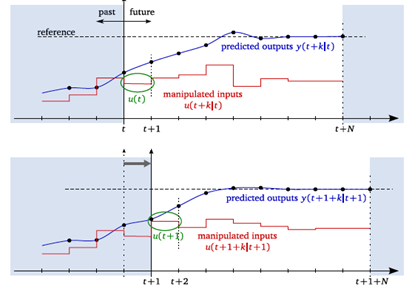
\includegraphics[width=0.75\textwidth]{01_rec_horizon.png}
\caption{Postupujúci horizont riadenia}
\label{01_rec_horizon}
\end{figure}
Nech existuje lineárny dynamický model s časovo invariantnými parametrami, vyjadrený diskrétnou stavovou rovnicou:
\begin{equation} \label{eq1}
\begin{split}
x(t+1)=Ax(t)+Bu(t), \\
y(t)=Cx(t)+Du(t), \\
x(t)∈R^n, y(t)∈R^P, u(t)∈R^m, \\
A∈R^{(n×n)}, B∈R^{(n×m)}, C∈R^{(p×n)}
\end{split}
\end{equation}
x, y, u sú stavy systému, výstupy systému a riadiace zásahy v uvedenom poradí v čase alebo lepšie povedané vo vzorke t. \\
n – predstavuje počet stavov systému \\
p – predstavuje počet výstupov \\
m – predstavuje počet vstupov \\
Matice A, B, C sú systémová matica, vstupná matica a výstupná matica v uvedenom poradí. System \ref{eq1} musí spĺňať nasledujúce obmedzenia na stav a vstup:
\begin{equation} \label{eq2}
\begin{split}
x(t)∈X,u(t)∈U \\
U⊂R^m \\
X⊂R^n
\end{split}
\end{equation}
kde obmedzujúca množina riadiacich zásahov U je konvexná, kompaktná (uzavretá a ohraničená) a obmedzujúca množina stavov X je konvexná a uzavretá. Pre obidve množiny U a X sa predpokladá, že obsahujú počiatok v ich vnútri.\cite{MPC04}
Najskôr je jednoduchšie vyriešiť optimálne riadenie bez obmedzení. Pozornosť bude upriamená na nájdenie takej optimálnej postupností $u^*$(k), ..., $u^*$(k+N – 1), ktorá bude minimalizovať zvolené kvadratické kritérium a zároveň rešpektovať dynamiku systému. Čo inými slovami znamená, že tento regulátor sa bude snažiť minimalizovať stav a rovnako riadiaci zásah, ešte lepšie povedané ich kvadrát. Ak by teda nebola špecifikovaná referenčná hodnota, ktorú má výstup regulátora sledovať, tak implicitne výstupná veličina prediktívneho regulátora konverguje k hodnote 0 alebo pri systémoch s viacerými výstupmi k nulovému vektoru.\\
N – predstavuje horizont predikcie. Ak je teda systém v stave $x_0$, ktorý poznáme a horizont predikcie je 3, tak do optimalizačnej funkcie vstupujú premenné $x_1$, $x_2$, $x_3$ a $u_1$, $u_2$, $u_3$ kde $u_1$ zabezpečí prechod do stavu $x_1$, $u_2$ do stavu $x_2$ atď. každá premenná x je odvoditeľná z predošlého stavu a prvý stav $x_0$ je známy. Preto jedinou ,,neznámou`` ostáva sekvencia riadiacich zásahov. Jedna z otázok by mohla byť, prečo sa využíva kvadratické kritérium. Ako odpoveď je možné použiť príklad kvality riadenia. Pri hodnotení kvality riadenia sa používajú integrálne kritéria. Existuje jednoduché kritérium, ktoré spraví integrál pod krivkou regulačnej odchýlky. Nevýhodou tohto je, že ak dochádza k preregulovaniu a regulačná odchýlka je záporná, veľkosť plochy je zmenšovaná o tie časti, ktoré sú záporné. Toto sa rieši absolútnym integrálnym kritériom, ktoré spraví zo zápornej regulačnej odchýlky kladnú a teda plocha pod krivkou sa zväčšuje aj pri preregulovaní. Navyše existuje kvadratické kritérium, ktoré okrem toho, že odstraňuje problém so zápornou regulačnou odchýlkou navyše viac penalizuje hodnoty odchýlky väčšie ako 1. Inými slovami, ak je hodnota viac ako 1 o to horšiu kvalitu regulácie bude toto kritérium indikovať. Problém so zápornou regulačnou odchýlkou je znázornený na obrázkoch \ref{02_reg_odch}, \ref{03_reg_odch} a \ref{04_reg_odch}.
\begin{figure}[!htbp]
\centering
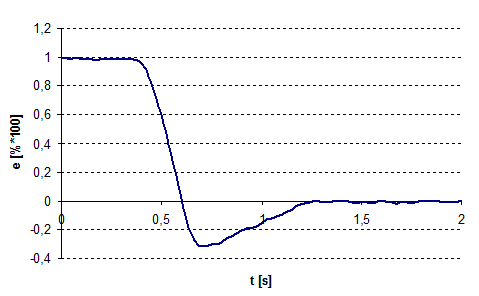
\includegraphics[width=0.90\textwidth]{02_reg_odch.png}
\caption{Hodnota regulačnej odchýlky v čase}
\label{02_reg_odch}
\end{figure}

\begin{figure}[!htbp]
\centering
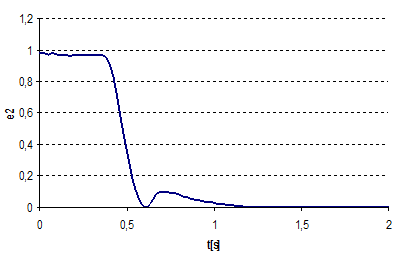
\includegraphics[width=0.90\textwidth]{03_reg_odch.png}
\caption{Časová závislosť kvadrátu regulačnej odchýlky}
\label{03_reg_odch}
\end{figure}
\begin{figure}[!htbp]
\centering
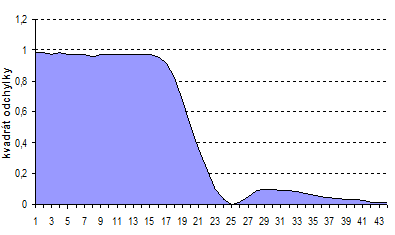
\includegraphics[width=0.90\textwidth]{04_reg_odch.png}
\caption{Plocha kvadrátu regulačnej odchýlky}
\label{04_reg_odch}
\end{figure}

Rovnako ako pri minimalizácii regulačnej odchýlky, tak aj pri minimalizácii riadiaceho zásahu je kvadratické kritérium najlepším ukazovateľom. \\
Pre porozumenie ďalších vzťahov si je potrebné uvedomiť, že: $x(t+k) =x_{(t+k)}$ \\
\begin{itemize}
\item Pre vzorku k = 0 (aktuálny stav systému): x(t)= $x_t$, 
\item pre vzorku k = 1 x(t+1)=$x_{(t+1)}$, 
\item atď.
\end{itemize}
Kvadratické kritérium pre konečný horizont predikcie dĺžky N je:
\begin{equation} \label{eq3}
\begin{split}
J(x(t),u(t),…,u(N-1))=\frac{1}{2}∑_{k=0}^{N-1}[x_k^T Qx_k+u_k^T Ru_k ] +  \frac{1}{2} x_N^T Q_N x_N
\end{split}
\end{equation}
kde:
\begin{equation} \label{eq4}
\begin{split}
x_(k+1)=Ax_k+Bu_k \\
x_0=x(t), \\
Q=Q^T  \succcurlyeq 0,Q_N=Q_N^T \succcurlyeq 0,R=R^T \succ 0 \\
Q_N∈R^{n×n} \\
R∈R^{m×m}
\end{split}
\end{equation}
Matice, Q, $Q_N$ a R sú nazývané váhové matice a spolu s horizontom predikcie N sú nazývané parametrami na ladenie prediktívneho regulátora. Nájdenie optimálneho riadenia, ktoré by minimalizovalo kvadratické kritérium predstavuje dynamickú optimalizáciu a má v tomto prípade aj analytické riešenie: \cite{MPC05}

\begin{equation} \label{eq5}
\begin{split}
x_{t+k}= A^k x_0+ ∑_{i=0}^{k-1}A^i Bu_{k-1-i}\\
u_{t,N}=[u_t^T,…,u_{t+N-1}^T  ]
\end{split}
\end{equation}

Vyjadrenie predikovaného stavu je potom:
\begin{equation} \label{eq6}
\begin{split}
[ x_{t+1}^T,…,x_{t+N}^T  ]^T=Vx_0+Tu_{t,N}
\end{split}
\end{equation}

Táto rovnica je jedna z najdôležitejších pri pochopení fungovania on-line prediktívneho algoritmu. Preto je vhodné ukázať ako matica V a T vyzerajú pre konkrétny jednoduchý systém s horizontom predikcie N = 3 zadaný v stavovom priestore:

\begin{equation} \label{eq7}
\begin{split}
A = \begin{bmatrix}
1 & 0 \\
1 & 1 \\
\end{bmatrix}, 
B = \begin{bmatrix}
0 \\
0,5 \\
\end{bmatrix} \\
C = \begin{bmatrix}
0 & 1 \\
\end{bmatrix}, D = 0 \\
x_{0} = \begin{bmatrix}
4 \\
5 \\
\end{bmatrix} = \begin{bmatrix}
x_{01} \\
x_{02} \\
\end{bmatrix}
\end{split}
\end{equation}
Matice V~a~T vyzerajú:
\begin{equation} \label{eq8}
\begin{split}
V = \begin{bmatrix}
\begin{matrix}
1 & 0 \\
1 & 1 \\
\end{matrix} \\
\begin{matrix}
1 & 0 \\
2 & 1 \\
\end{matrix} \\
\begin{matrix}
1 & 0 \\
3 & 1 \\
\end{matrix} \\
\end{bmatrix} = \begin{bmatrix}
A^{1} \\
A^{2} \\
A^{3} \\
\end{bmatrix} \\
T = \begin{bmatrix}
\begin{matrix}
1 & 0 & 0 \\
0,5 & 0 & 0 \\
\end{matrix} \\
\begin{matrix}
1 & 1 & 0 \\
1,5 & 0,5 & 0 \\
\end{matrix} \\
\begin{matrix}
1 & 1 & 1 \\
2,5 & 1,5 & 0,5 \\
\end{matrix} \\
\end{bmatrix} = \begin{bmatrix}
\begin{matrix}
A^{0}B & 0\  & 0 \\
\end{matrix} \\
\begin{matrix}
A^{1}B & A^{0}B & 0 \\
\end{matrix} \\
\begin{matrix}
A^{2}B & A^{1}B & A^{0}B \\
\end{matrix} \\
\end{bmatrix}
\end{split}
\end{equation}

Výsledný vzťah:
\begin{equation} \label{eq9}
\begin{split}
{\lbrack\ \begin{bmatrix}
x_{11} \\
x_{12} \\
\end{bmatrix},\ \begin{bmatrix}
x_{21} \\
x_{22} \\
\end{bmatrix},\begin{bmatrix}
x_{31} \\
x_{32} \\
\end{bmatrix}\rbrack}^{T} = \begin{bmatrix}
A^{1} \\
A^{2} \\
A^{3} \\
\end{bmatrix}\begin{bmatrix}
x_{01} \\
x_{02} \\
\end{bmatrix} + \begin{bmatrix}
\begin{matrix}
A^{0}B & 0\  & 0 \\
\end{matrix} \\
\begin{matrix}
A^{1}B & A^{0}B & 0 \\
\end{matrix} \\
\begin{matrix}
A^{2}B & A^{1}B & A^{0}B \\
\end{matrix} \\
\end{bmatrix}\begin{bmatrix}
u_{1} \\
u_{2} \\
u_{3} \\
\end{bmatrix}
\end{split}
\end{equation}
Dôležitý krok pri hľadaní optimálneho riadenia je zo vzťahu \ref{eq3}
„odstrániť`` sumu. Finálny vzťah vyzerá:
\begin{equation} \label{eq10}
\begin{split}
J\left( x\left( t \right),U_{t} \right) = \ \frac{1}{2}{u_{t,N}}^{T}Hu_{t,N} + x^{T}\left( t \right)FU_{t} + \frac{1}{2}x^{T}\left( t \right)\text{Yx}\left( t \right),
\end{split}
\end{equation}

Matica \(\ H \in R^{(m \bullet N \times m \bullet N)}\) ,
\(F \in R^{(n \times m \bullet N)}\), \(Y \in R^{(n \times n)}\). Ak sa
symbol \(\bigotimes\) označí ako kroneckerovo násobenie matíc a
\(I_{j} \in R^{(j \times j)}\), jednotková matica s~príslušnou
dimenziou, tak platí:

\begin{equation} \label{eq11}
\begin{split}
H = \ T^{T}\tilde{Q}T + \ I_{N}\ \bigotimes\ R,\ \ F = V^{T}\tilde{Q}T,\ \ Y = V^{T}\tilde{Q}V \\
\tilde{Q} = \ \begin{bmatrix}
I_{N - 1}\ \bigotimes\ Q & 0 \\
0 & Q_{N} \\
\end{bmatrix}
\end{split}
\end{equation}

Pre systém zo vzťahu \ref{eq7} a~váhy \(Q = Q_{N} = I_{2},\ R = 0,1\) budú
jednotlivé matice vyzerať:

\begin{equation} \label{eq12}
\begin{split}
H = \ \begin{bmatrix}
11,85 & 6,5 & 2,25 \\
6,5 & 4,6 & 1,75 \\
2,25 & 1,75 & 1,35 \\
\end{bmatrix}, F = \begin{bmatrix}
14 & 7,5 & 2,5 \\
4,5 & 2 & 0,5 \\
\end{bmatrix}, \\
Y = \ \ \begin{bmatrix}
17 & 6 \\
6 & 3 \\
\end{bmatrix}
\end{split}
\end{equation}

Optimálnu riadiacu sekvenciu je možné dostať minimalizáciou kvadratickej
formy \ref{eq10}:

\begin{equation} \label{eq13}
\begin{split}
u_{t,N}^{*}\left( x\left( t \right) \right) = \arg{\min_{u_t,N}{\{ J(x\left( t \right),u_{t,N}\ \}}} = - H^{- 1}F^{T}x(t)
\end{split}
\end{equation}

Optimálna hodnota kritéria je:

\begin{equation} \label{eq14}
\begin{split}
J^{*}\left( x\left( t \right) \right) = \min_{u_t,N}{\{ J(x\left( t \right),u_{t,N}\ \}} = \frac{1}{2}x^{T}(t)(Y - FH^{- 1}F^{T})x(t)
\end{split}
\end{equation}

Na to aby sa zabezpečila spätná väzba, je potrebné v~každom kroku použiť
iba prvú hodnotu zo sekvencie riadiacich zásahov a~potom zmerať stav
a~na základe tej hodnoty znovu vypočítať optimálnu sekvenciu riadiacich
zásahov. Bez merania stavu, by to bola regulácia v~otvorenom regulačnom
obvode. Meranie stavu a~jeho použitie pri výpočte nasledujúceho
riadiaceho zásahu v~každom kroku zabezpečí reguláciu v~uzavretom
regulačnom obvode.

\subsubsection{On-line MPC s obmedzením}

Doteraz sa reguloval systém, v~ktorom nebolo žiadne obmedzenie.
V~realite ich však býva mnoho. Pokiaľ sa pri návrhu regulátora začnú
brať do úvahy rovnice \ref{eq2}, bude ich treba zapracovať do výpočtu. Pri
návrhu prediktívneho regulátora s~obmedzením sa využíva kvadratické
programovanie. Úloha kvadratického programovania je úlohou nelineárneho
programovania, v~ktorej sústava ohraničení je lineárna a~účelová funkcia
je kvadratická. Všeobecná formulácia kvadratickej úlohy je:

\begin{equation} \label{eq15}
\begin{split}
f\left( x \right) = \min_{x}\left\{ x^{T}Hx + F^{T}\text{x\ } \right\} \\
x \in D = \{\operatorname{x|}{\ \ Lx \leq m_{c}},\ x \geq 0\}
\end{split}
\end{equation}

Pre návrh regulátora je premenná, ktorej minimum sa hľadá, sekvencia
riadiacich zásahov \(u_{t,N}^{*}\). Rovnice pre prediktívny regulátor
s~obmedzením následne vyzerajú:

\begin{equation} \label{eq16}
\begin{split}
J\left( x\left( t \right),\ u\left( t \right),\ldots,\ u\left( N - 1 \right) \right) = \frac{1}{2}\sum_{k = 0}^{N - 1}\left\lbrack x_{k}^{T}Qx_{k} + u_{k}^{T}Ru_{k} \right\rbrack + \ \frac{1}{2}x_{N}^{T}Q_{N}x_{N}
\end{split}
\end{equation}

kde:
\begin{equation} \label{eq17}
\begin{split}
x_{k + 1} = Ax_{k} + Bu_{k}, \\
x_{0} = x\left( t \right), \\
E_{c}x_{k} + G_{c}u_{k} \leq m_{c},\ \ k = 1\ldots N \\
Q = Q^{T} \succcurlyeq 0,\ Q_{N} = Q_{N}^{T} \succcurlyeq 0,\ R = R^{T} \succ 0
\end{split}
\end{equation}

Aby bolo možné sústavu rovníc \ref{eq16} a \ref{eq17} zapracovať do kvadratického programovania, previesť do maticového tvaru. Prvá časť rovnice ostáva nezmenená, pridá sa k~nej druhá časť:

\begin{equation} \label{eq18}
\begin{split}
J\left( x\left( t \right),U_{t} \right) = \ \frac{1}{2}{u_{t,N}}^{T}Hu_{t,N} + x^{T}\left( t \right)FU_{t} + \frac{1}{2}x^{T}\left( t \right)\text{Yx}\left( t \right), \\
Gu_{t,N} \leq w + Ex(t)
\end{split}
\end{equation}

Kde matice H, F, Y sú určené rovnako ako vo vzťahu \ref{eq11} a~matice G, E, a
vektor w majú tvar:

\begin{equation} \label{eq19}
\begin{split}
G = \begin{bmatrix}
{- I}_{N} \\
\begin{matrix}
I_{N} \\
 - (I_{N}\bigotimes CT) \\
\end{matrix} \\
\begin{matrix}
(I_{N}\bigotimes CT) \\
 \vdots \\
\end{matrix} \\
\end{bmatrix},\ E = \begin{bmatrix}
0 \\
\begin{matrix}
0 \\
 - (I_{N}\bigotimes CV) \\
\end{matrix} \\
\begin{matrix}
(I_{N}\bigotimes CV) \\
 \vdots \\
\end{matrix} \\
\end{bmatrix},\ w = \begin{bmatrix}
 - (1_{N}\bigotimes u_{\min}) \\
\begin{matrix}
(1_{N}\bigotimes u_{\max}) \\
 - (1_{N}\bigotimes y_{\min}) \\
\end{matrix} \\
\begin{matrix}
(1_{N}\bigotimes y_{\max}) \\
 \vdots \\
\end{matrix} \\
\end{bmatrix}
\end{split}
\end{equation}

V rovnici \ref{eq19} sú znázornené základné systémové obmedzenia. Môže
existovať ďaleko viac. \(1_{N}\) predstavuje jednotkový vektor
o~veľkosti N. Prvé dva riadky matice G, \(G_{1,2} \in R^{N \times N}\),
E, \(E_{1,2} \in R^{N \times n}\) a~vektor w, \(w_{1,2} \in R^{N}\) v
(19) predstavujú obmedzenia vstupu. Druhé dva riadky matice G,
\(G_{3,4} \in R^{N \times N}\), E, \(E_{3,4} \in R^{N \times n}\)
a~vektor w, \(w_{3,4} \in R^{N}\) v \ref{eq19} predstavujú obmedzenia výstupu.
Ďalšie obmedzenia, by museli nadobúdať rovnaké rozmery ako predošlé
riadky príslušných matíc a~vektora.

Ak sa pridajú do systému \ref{eq7} obmedzenia na vstup a~výstup:

\begin{equation} \label{eq20}
\begin{split}
- 1 \leq u\left( t \right) \leq 1,\ \  - 10 \leq y\left( t \right) \leq \ 10
\end{split}
\end{equation}

matice G, E a vektor~w budú vyzerať:

\begin{equation} \label{eq21}
\begin{split}
G = \begin{bmatrix}
{- I}_{3} \\
I_{3} \\
\begin{matrix}
 - (I_{3}\bigotimes CT) \\
(I_{3}\bigotimes CT) \\
\end{matrix} \\
\end{bmatrix},\ E = \begin{bmatrix}
0 \\
\begin{matrix}
0 \\
 - (I_{3}\bigotimes CV) \\
\end{matrix} \\
\begin{matrix}
(I_{3}\bigotimes CV) \\
 \vdots \\
\end{matrix} \\
\end{bmatrix},\ m_{c} = \begin{bmatrix}
 - (1_{3}\bigotimes u_{\min}) \\
(1_{3}\bigotimes u_{\max}) \\
\begin{matrix}
 - (1_{3}\bigotimes y_{\min}) \\
(1_{3}\bigotimes y_{\max}) \\
\end{matrix} \\
\end{bmatrix}
\end{split}
\end{equation}

\begin{equation} \label{eq22}
\begin{split}
G = \begin{bmatrix}
 - \begin{pmatrix}
1 & 0 & 0 \\
0 & 1 & 0 \\
0 & 0 & 1 \\
\end{pmatrix} \\
\begin{pmatrix}
1 & 0 & 0 \\
0 & 1 & 0 \\
0 & 0 & 1 \\
\end{pmatrix} \\
\begin{matrix}
 - \begin{pmatrix}
0,5 & 0 & 0 \\
1,5 & 0,5 & 0 \\
2,5 & 1,5 & 0,5 \\
\end{pmatrix} \\
\begin{pmatrix}
0,5 & 0 & 0 \\
1,5 & 0,5 & 0 \\
2,5 & 1,5 & 0,5 \\
\end{pmatrix} \\
\end{matrix} \\
\end{bmatrix},\ E = \begin{bmatrix}
 - \begin{pmatrix}
0 & 0 \\
0 & 0 \\
0 & 0 \\
\end{pmatrix} \\
\begin{pmatrix}
0 & 0 \\
0 & 0 \\
0 & 0 \\
\end{pmatrix} \\
\begin{matrix}
 - \begin{pmatrix}
1 & 1 \\
2 & 1 \\
3 & 1 \\
\end{pmatrix} \\
\begin{pmatrix}
1 & 1 \\
2 & 1 \\
3 & 1 \\
\end{pmatrix} \\
\end{matrix} \\
\end{bmatrix},\ w = \begin{bmatrix}
\begin{pmatrix}
1 \\
1 \\
\end{pmatrix} \\
\begin{pmatrix}
1 \\
1 \\
\end{pmatrix} \\
\begin{matrix}
\begin{pmatrix}
10 \\
10 \\
\end{pmatrix} \\
\begin{pmatrix}
10 \\
10 \\
\end{pmatrix} \\
\end{matrix} \\
\end{bmatrix}
\end{split}
\end{equation}

Vznikne sústava lineárnych rovníc, ktoré tvoria obmedzenia pre
kvadratický problém.

\begin{equation} \label{eq23}
\begin{split}
\begin{bmatrix}
 - \begin{pmatrix}
1 & 0 & 0 \\
0 & 1 & 0 \\
0 & 0 & 1 \\
\end{pmatrix} \\
\begin{pmatrix}
1 & 0 & 0 \\
0 & 1 & 0 \\
0 & 0 & 1 \\
\end{pmatrix} \\
\begin{matrix}
 - \begin{pmatrix}
0,5 & 0 & 0 \\
1,5 & 0,5 & 0 \\
2,5 & 1,5 & 0,5 \\
\end{pmatrix} \\
\begin{pmatrix}
0,5 & 0 & 0 \\
1,5 & 0,5 & 0 \\
2,5 & 1,5 & 0,5 \\
\end{pmatrix} \\
\end{matrix} \\
\end{bmatrix}\begin{bmatrix}
u_{1} \\
u_{2} \\
u_{3} \\
\end{bmatrix} \leq \begin{bmatrix}
\begin{pmatrix}
1 \\
1 \\
\end{pmatrix} \\
\begin{pmatrix}
1 \\
1 \\
\end{pmatrix} \\
\begin{matrix}
\begin{pmatrix}
10 \\
10 \\
\end{pmatrix} \\
\begin{pmatrix}
10 \\
10 \\
\end{pmatrix} \\
\end{matrix} \\
\end{bmatrix} + \begin{bmatrix}
 - \begin{pmatrix}
0 & 0 & 0 \\
0 & 0 & 0 \\
0 & 0 & 0 \\
\end{pmatrix} \\
\begin{pmatrix}
0 & 0 & 0 \\
0 & 0 & 0 \\
0 & 0 & 0 \\
\end{pmatrix} \\
\begin{matrix}
 - \begin{pmatrix}
1 & 1 \\
2 & 1 \\
3 & 1 \\
\end{pmatrix} \\
\begin{pmatrix}
1 & 1 \\
2 & 1 \\
3 & 1 \\
\end{pmatrix} \\
\end{matrix} \\
\end{bmatrix}\begin{bmatrix}
x_{01} \\
x_{02} \\
\end{bmatrix}
\end{split}
\end{equation}

Ak sú obmedzenia na systém príliš striktné, môže sa stať, že kvadratický
problém nemá riešenie. Takáto situácia je znázornená na obrázku \ref{05_restric}.

\begin{figure}[!htbp]
\centering
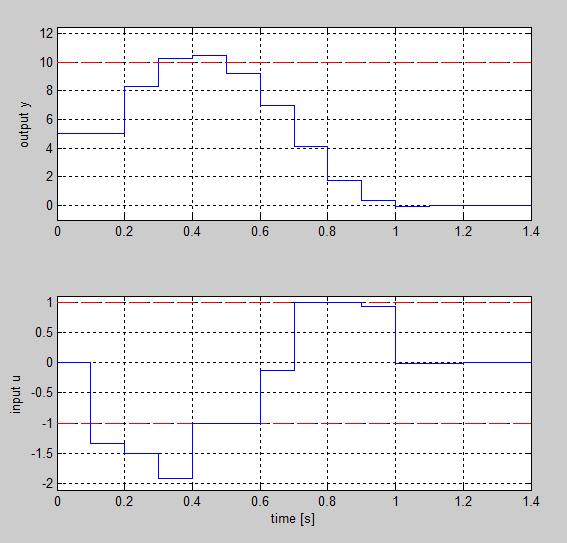
\includegraphics[width=0.99\textwidth]{05_restric.png}
\caption{Časový priebeh výstupnej veličiny a riadiaceho zásahu pre neriešiteľný kvadratický problém. Červená čiara predstavuje obmedzenie na danú veličinu}
\label{05_restric}
\end{figure}

Ak by obmedzenia na výstup boli napríklad
\(- 13 \leq y\left( t \right) \leq \ 13\), kvadratický problém by bol
riešiteľný a~jeho riešenie pre horizont predikcie 3 je zobrazene na
obrázku \ref{06_restric_ok}.

\begin{figure}[!htbp]
\centering
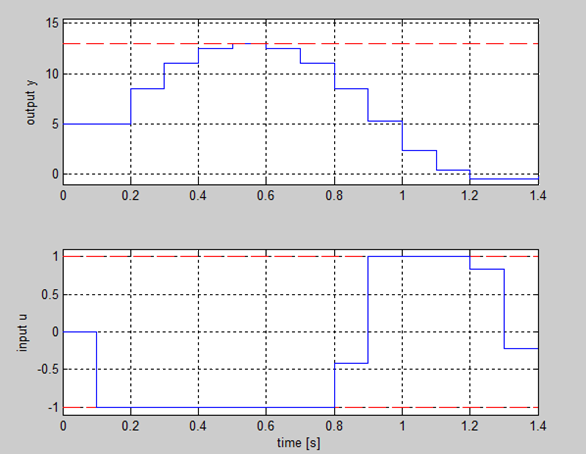
\includegraphics[width=0.99\textwidth]{06_restric_ok.png}
\caption{Časový priebeh výstupnej veličiny a riadiaceho zásahu riešiteľného kvadratického problému}
\label{06_restric_ok}
\end{figure}

\subsubsection{On-line MPC so sledovaním referenčného signálu}
Doteraz bol riešený regulátor, ktorý reguloval hodnotu k „počiatku``
k~hodnote 0 alebo nulovému vektoru. Táto kapitola obsahuje návrh MPC
regulátora, ktorý bude sledovať po častiach konštantný referenčný signál
r(t). Stále sa berie do úvahy systém \ref{eq1}. Najprv je potrebné nahradiť
člen \(x_{k}^{T}Qx_{k}\) v~pôvodnom kritériu \ref{eq17} odchýlkou

\begin{equation} \label{eq24}
\begin{split}
{(z_{k} - r_{k})}^{T}Q_{y}(z_{k} - r_{k})
\end{split}
\end{equation}

kde

\begin{equation} \label{eq25}
\begin{split}
z\left( t \right) = Zy\left( t \right),\ z\left( t \right) \in R^{p_{z}},\ p_{z} \leq p,\ r \leq m
\end{split}
\end{equation}

Aby to bolo možné, je potrebné poznať predikovanú hodnotu referenčného
signálu. Ta môže byť definovaná rôznymi spôsobmi jedna z~možností:
r(t+1)=r(t).

V~ustálenom stave je potrebné, aby platila rovnosť \(z_{u} = r_{u}\).
Takže:

\begin{equation} \label{eq26}
\begin{split}
\begin{bmatrix}
I_{n} - A & - B \\
\text{ZC} & 0 \\
\end{bmatrix}\ \begin{bmatrix}
x_{u} \\
u_{u} \\
\end{bmatrix} = \begin{bmatrix}
0 \\
r_{u} \\
\end{bmatrix}
\end{split}
\end{equation}


Ak ma predchádzajúca matica plnú riadkovú hodnosť, existuje riešenie \(u_{u}\)
a \(x_{u}.\). V~dôsledku nenulového ustáleného vstupu sa v~praxi často
používa odchýlka \(u_{k} = u_{k} - u_{k - 1}\). Ak sústava obsahuje
integrátor, je lepšie použiť hodnotu u. \cite{MPC05}

Kritérium pre sledovanie referencie má tvar:

\begin{equation} \label{eq27}
\begin{split}
J\left( x\left( t \right),\ u\left( t \right),\ldots,\ u\left( N - 1 \right) \right) = \frac{1}{2}\sum_{k = 0}^{N - 1}\left\lbrack e_{k}^{T}Q_{e}e_{k} + u_{k}^{T}Ru_{k} \right\rbrack
\end{split}
\end{equation}

kde 

\begin{equation} \label{eq28}
\begin{split}
e_{k} = y_{k} - r_{k}
\end{split}
\end{equation}

je regulačná odchýlka a

\begin{equation} \label{eq29}
\begin{split}
\Delta u_{k} = u_{k} - u_{k - 1}
\end{split}
\end{equation}

je optimalizovaná premenná. Systém rozšírený o~históriu riadiaceho
zásahu \(u_{k}\) a~generátor referencie \(r_{k}\) je formulovaný:

\begin{equation} \label{eq30}
\begin{split}
\begin{bmatrix}
x_{k + 1} \\
u_{k} \\
r_{k + 1} \\
\end{bmatrix} = \begin{bmatrix}
A & B & 0 \\
0 & I_{m} & 0 \\
0 & 0 & I_{n_{y}} \\
\end{bmatrix}\ \begin{bmatrix}
x_{k} \\
u_{k - 1} \\
r_{k} \\
\end{bmatrix} + \begin{bmatrix}
B \\
I_{m} \\
0 \\
\end{bmatrix}u_{k} = \ A_{m}\hat{x_{k}} + B_{m}u_{k} \\
e_{k} = \begin{bmatrix}
C & 0 & - I_{n_{y}} \\
\end{bmatrix}\hat{x_{k}} = C_{m}\hat{x_{k}}
\end{split}
\end{equation}

\begin{figure}[!htbp]
\centering
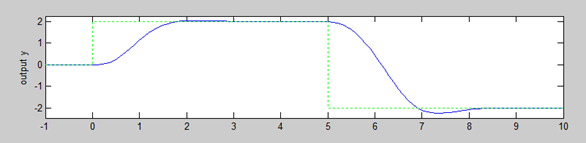
\includegraphics[width=0.99\textwidth]{07_ref.png}
\caption{Sledovanie referencie,  časové priebehy -  zelená referencia, modrá výstup systému}
\label{07_ref}
\end{figure}

Po upravení algoritmu na sledovanie po častiach spojitého referenčného signálu už MPC regulátor neriadi výstupnú veličinu k 0 hodnote alebo nulovému vektoru, ale ku aktuálnej hodnote prípadne vektoru referenčného signálu v kroku k, \dots, k + N - 1, kde N predstavuje horizont predikcie. Preto referenčný signál vstupujúci do výpočtu je je buď vektor pre jednorozmerné systémy (SISO) alebo matica pre viacrozmerné systémy (MIMO). Časový priebeh výstupnej veličiny SISO systému regulovaného MPC regulátorom so sledovaním referencie je znázornený na obrázku \ref{07_ref}.

\subsubsection{Explicitné riešenie - offline MPC} \label{offmpc}

Je zrejmé, že optimálna hodnota kritéria \ref{eq14} a~optimálna riadiaca sekvencia \ref{eq13} (aj s~obmedzeniami) sú funkciou stavu x(t). Túto úlohu je možné formulovať pomocou \textbf{multiparametrického kvadratického
programovania} (mp-QP), ktoré sa snaží nájsť optimálne riešenie pre
všetky možné hodnoty parametra x(t) vopred. Ak sa spraví substitúcia
rovnice

\begin{equation} \label{eq31}
\begin{split}
J^{*}\left( x\left( t \right) \right) = \min_{u_t,N}\left\{ J\left( x\left( t \right),u_{t}) \right|Gu_{t} \leq W + Ex(t) \right\}
\end{split}
\end{equation}

pomocou

\begin{equation} \label{eq32}
\begin{split}
u_{t} = \tilde{u_{t}} - H^{- 1}F^{T}x(t)
\end{split}
\end{equation}

vznikne:

\begin{equation} \label{eq33}
\begin{split}
J^{*}\left( x\left( t \right) \right) = \min_{u_t,N}\left\{ J\left( \tilde{u_{t}},x\left( t \right)) = \frac{1}{2}{\tilde{u}}_{t}^{T}H{\tilde{u}}_{t} + \beta \right|G{\tilde{u}}_{t} \leq W + Sx(t) \right\}
\end{split}
\end{equation}

Kde \(S = E + GH^{- 1}F^{T}\)
a~\(\beta = \frac{1}{2}{x\left( t \right)}^{T}\left( FH^{- 1}F^{T} + Y \right)x(t)\).
Ešte je potrebné zaviesť množinu indexov
I\(= \left\{ 1,\ldots,\ q \right\},\ \)ktorá zodpovedá riadkom matice G,
W a S. \\
Kritický región CR je taká polytopická oblasť v~priestore parametrov
x(t), ktorá má v~optimálnej hodnote
\(J^{*}\left( x\left( t \right) \right),\ u^{*}\left( x\left( t \right) \right)\)
aktívne rovnaké obmedzenia \(A(x(t)) \subset I\). Takže platí

\begin{equation} \label{eq34}
\begin{split}
G_{A}{\tilde{u_{t}}}^{*}\left( x\left( t \right) \right) = W_{A} + S_{A}x\left( t \right)\ pre\ x(t) \in CR
\end{split}
\end{equation}

Nech \(H \succ 0\) a~nech \(G_{A}\)majú lineárne nezávisle riadky, potom
optimálna sekvencia
\({\tilde{u_{t}}}^{*}\left( x\left( t \right) \right)\) je jednoznačne
definovaná afinnou funkciou stavu x(t) na danom kritickom regióne CR.

\begin{equation} \label{eq35}
\begin{split}
{\tilde{u_{t}}}^{*}\left( x\left( t \right) \right) = H^{- 1}G_{A}^{T}(G_{A}H^{- 1}G_{A}^{T})(W_{A} + S_{A}x\left( t \right))
\end{split}
\end{equation}

Ak sa preformuluje optimalizačný problém \ref{eq13} (s obmedzeniami) ako mp-QP
a \(H \succ 0\), potom optimálna riadiaca sekvencia
\({u_{t}}^{*}\left( x\left( t \right) \right):X_{\text{feas}} \rightarrow R^{m}\)
je spojitá, po častiach afinná funkcia na polyedry a~optimálna hodnota
\(J^{*}(x\left( t \right))\) je spojitá, konvexná a~po častiach
kvadratická funkcia na polyedry.

Algoritmus mp-QP najskôr spočíta riešenie (13) (s obmedzeniami) pre
vhodne zvolenú počiatočnú podmienku (\(x_{0} \in X_{\text{feas}}\))
a~vytvorí sa príslušný kritický región CR\textsubscript{0}. Potom
rekurzívne prehľadá okolie a~vytvára nové regióny. Výsledkom je
rozdelenie oblasti \(X_{\text{feas}}\)do kritických regiónov
\(CR_{i} = \left\{ x \right|P_{i}x \leq p_{i}\}\), nad ktorými je
definovaná spojitá afinná funkcia:

\begin{equation} \label{eq36}
\begin{split}
{u_{t}}^{*}\left( x\left( t \right) \right) = F_{i}x\left( t \right) + G_{i}
\end{split}
\end{equation}

a spojitá kvadratická funkcia

\begin{equation} \label{eq37}
\begin{split}
{J_{t}}^{*}\left( x\left( t \right) \right) = x^{T}\left( t \right)A_{i}x\left( t \right) + B_{i}x\left( t \right) + C_{i}
\end{split}
\end{equation}

Týmto sa presunula numerická výpočtová náročnosť optimalizácie \ref{eq13} k~off-line výpočtom. V~priebehu riadenia stačí identifikovať región CR\textsubscript{i}, obsahujúci aktuálny stav x(t) a~aplikovať príslušný
zákon riadenia \label{eq36}. \cite{MPC05} \\
Takýmto spôsobom je možné rozdeliť výpočtovú zložitosť na dve časti. Prvá, výpočtovo zložitejšia, časť je hľadanie kritických regiónov, ktorá sa môže uskutočniť pred zavedením regulátora do behu. Tuto nie je čas kritický, pretože regulačný proces nebeží. Druhá časť je počas behu regulačného procesu. Tá predstavuje časovo nenáročnú operáciu vyhľadania kritického regiónu v pamäti a podľa neho vrátiť akčný zásah. Hlavná nevýhoda offline - explicitného riešenia je, že systém je jednorázovo daný a už počas behu nevstupuje do výpočtu na rozdiel od online riešenia, kde do každého kroku matematický model systému vstupuje a teda je možné  matematický model dynamicky adaptovať, aby čo najviac zodpovedal reálnemu systému. Pri voľbe spôsobu implementácie praktickej časti pre výučbu aj neskôr v IoT prostredí, tento fakt zavážil a zvolila sa online metóda implementácie.
\subsection{Opis funkčnosti On-line MPC algoritmu} \label{mpcalg}
Vytvorený algoritmus sa skladá skladá z viacerých modulov - funkcií naprogramovaných v prostredí Matlab a prispôsobených na fungovanie v open source verzii Octave. Program bol vytvorený pre účely využitia v pedagogickom procese. Grafické rozhranie bolo vytvorené pomocou komponent Matlabu - Guide, ktorý slúži práve na vytváranie grafických rozhraní. Základné komponenty, z ktorých sa program skladá sú znázornené na obrázku \ref{16_com}.
\begin{figure}[!htbp]
\centering
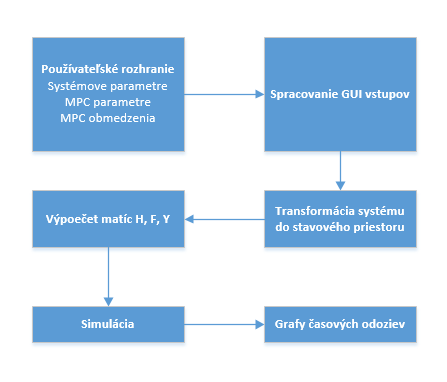
\includegraphics[width=0.8\textwidth]{16_com.png}
\caption{Základné komponenty}
\label{16_com}
\end{figure}

\begin{enumerate}
  \item
    Používateľské rozhranie je popísane v kapitole \ref{mpcprogram}
  \item
    Spracovanie vstupov zabezpečí správnu konverziu reťazcov na čísla a výsledné čísla priradí do správnych premenných potrebných na vstupe do ďalšej časti.
  \item
    MPC regulátor pre svoje fungovanie vždy potrebuje mať na vstupe   matematický model systému podľa rovnice \ref{eq1}, ktorý sa označuje ako systém zadaný v stavovom priestore. Táto časť zabezpečí konverziu z prenosovej funkcie na stavový priestor.
  \item
   Nasleduje výpočet matíc H, F, Y podľa rovníc \ref{eq11}, ktoré sú produktom matíc A, B, C z rovnice \ref{eq1} a váhových matíc, Q, $Q_n$ a R z rovnice \ref{eq11}, ktoré si používateľ volí.
   \item
   Následne prebieha simulácia, ktorej komponenty sú znázornené na obrázku \ref{17_dsim} a popísane nižšie.
   \item
   Produktom simulácie sú dáta, ktoré vytvoria grafy časových odoziev popísaných v kapitole \ref{mpcprogram}.
\end{enumerate}

\begin{figure}[!htbp]
\centering
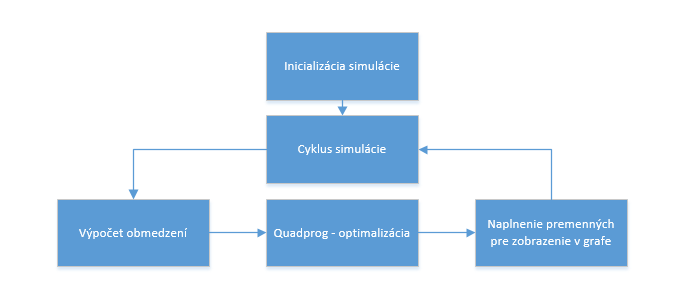
\includegraphics[width=1.1\textwidth]{17_dsim.png}
\caption{Detail komponentu simulácia}
\label{17_dsim}
\end{figure}
\begin{enumerate}
  \item
	Počas inicializácie simulácie sa pripravuje referenčný signál, počiatočný stav systému a počet krokov simulácie.
  \item
    Počet krokov simulácie je nastavený na podiel času simulácie a periódy vzorkovania.
  \item
    V prvej fáze simulačného cyklu sa prepočítajú obmedzenia systému podľa rovnice \ref{eq19}.
  \item 
    Následne prebehne samotná optimalizácia spustením Matlab súčasti \textit{quadprog}, prípade Octave súčasti \textit{qp}. Bez obmedzení by to bol výpočet podľa rovnice \ref{eq13} spomenuté súčasti kvadratického programovania k tomu pridajú sústavu obmedzení.
  \item
    Po optimalizácii sa vyberie prvý akčný zásah z vektora akčných zásahov, ktorý má dĺžku horizontu predikcie, čo je vlastne výsledok optimalizácie. Keďže v programe beží simulačný cyklus tak sa vypočíta výstup, a stav, ktoré sa zapamätajú a následne začína ďalší krok simulačného cyklu.
\end{enumerate}


\subsection{Overenie On-line MPC algoritmu} \label{mpcprogram}
Po teoretickom základe a popise vytvoreného algoritmu nasleduje popis grafického rozhrania a jeho overenie. Grafické rozhranie vytvoreného programu je znázornené na obrázku \ref{08_gui} 

\begin{figure}[!htbp]
\centering
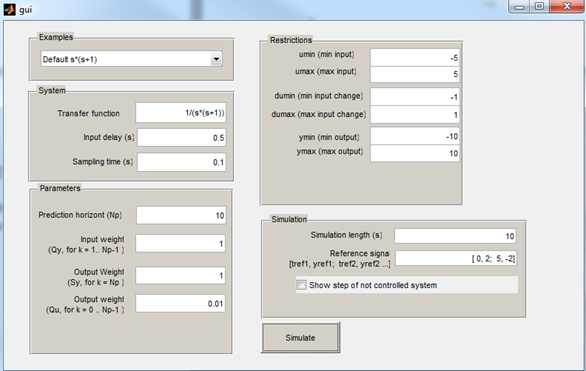
\includegraphics[width=0.99\textwidth]{08_gui.png}
\caption{Grafické rozhranie k programu na testovanie MPC algoritmu.}
\label{08_gui}
\end{figure}

a ponúka pre používateľa možnosti zadania:

\begin{itemize}
\item
  Systémových nastavení:

  \begin{itemize}
  \item
    Automatický vyplniť určité druhy systému
  \item
    Zadať akúkoľvek prechodovú funkciu v~s~alebo z~oblasti systému,
    ktorý má byť riadený
  \item
    Zadať dopravné oneskorenie systému
  \item
    ~periódu vzorkovania
  \end{itemize}
\item
  Ladiace parametre

  \begin{itemize}
  \item
    ~váha vstupu
  \item
    ~váha výstupu pre budúce hodnoty v kroku k=0 \dots N-1, N je horizont predikcie.
  \item
    ~váha výstupu pre budúcu hodnotu v kroku k=N, kde N je horizont predikcie
  \end{itemize}
\item
  Obmedzenia systému

  \begin{itemize}
  \item
    ~minimálny vstup
  \item
    ~maximálny vstup
  \item
    ~minimálna zmena vstupu
  \item
    ~maximálna zmena vstupu
  \item
    minimálny~výstup systému
  \item
    ~maximálny výstup systému
  \end{itemize}
\item
  Parametre simulácie

  \begin{itemize}
  \item
    ~čas simulácie
  \item
    ~referenčný signál zadávaný vo forme vektora dvojice hodnôt, kde prvá
    identifikuje čas, kedy ma zmena nastať a~druhá hodnota veľkosť
    skoku.
  \end{itemize}
\end{itemize}

Výstup z~grafického rozhrania po ponechaní prednastavených hodnôt sú grafy zobrazené na obrázku  \ref{09_out}.

\begin{figure}[!htbp]
\centering
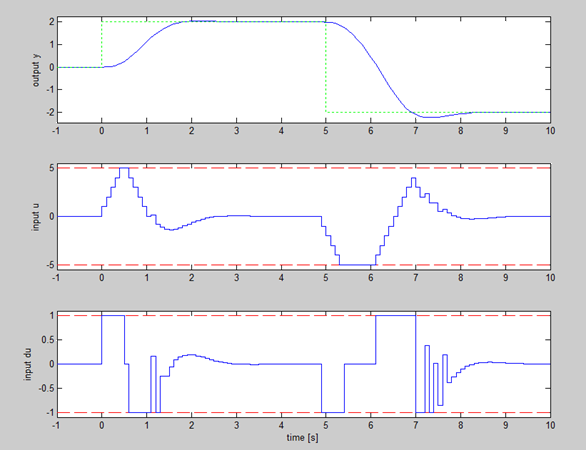
\includegraphics[width=0.99\textwidth]{09_out.png}
\caption{Časové priebehy výstupu systému, riadiaceho zásahu a zmeny riadiaceho zázsahu.}
\label{09_out}
\end{figure}


V~prvom grafe obrázku  \ref{09_out} je znázornený časový priebeh sledovania referenčnej hodnoty výstupnou veličinou. Zelenou farbou je referenčná veličina a výstupna veličina modrou.
V~druhom grafe obrázku  \ref{09_out} je znázornený
riadiaci zásah systému modrou farbou a~obmedzenia riadiaceho zásahu červenou farbou. V~treťom grafe obrázku  \ref{09_out} je znázornená zmena riadiaceho zásahu modrou farbou
a~obmedzenia červenou. Hodnotenie kvality regulácie priamymi ukazovateľmi \cite{MPC06}

\begin{itemize}
  \item Doba regulácie:
    \begin{itemize}
  		\item
    	Pre zmenu v čase 0s (zmena 1.) z hodnoty 0 na 2 je doba regulácie 2 sekundy
    	\item
    	Pre zmenu v čase 5s (zmena 2.) z hodnoty 2 na -2 je doba regulácie 3 sekundy
	\end{itemize}
  \item Preregulovanie:
    \begin{itemize}
  		\item
    	Pre zmenu 1. došlo k minimálnemu preregulovaniu.
    	\item
    	Pre zmenu 2. je preregulovanie badateľné.
	\end{itemize}  
  \item Regulačná odchýlka:
    \begin{itemize}
  		\item
    	Regulačná odchýlka je pre oba prípady 0.
	\end{itemize}   
\end{itemize}

Nie je tu porovnanie voči iným regulátorom, pretože to nie je zámerom tejto kapitoly. Kapitola slúži na demonštráciu funkčnosti predchádzajúcej teórie. Čo je však dôležité na tomto mieste zdôrazniť je znázornenie ako vplývajú obmedzenia na riadenie systému. 

\begin{figure}[!htbp]
\centering
\begin{subfigure}{.5\textwidth}
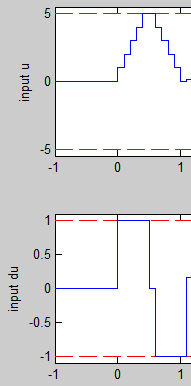
\includegraphics[width=0.5\linewidth]{10_steps.png}
\caption{Zapnuté obmedzenie}
\label{10_steps}
\end{subfigure}%
\begin{subfigure}{.5\textwidth}
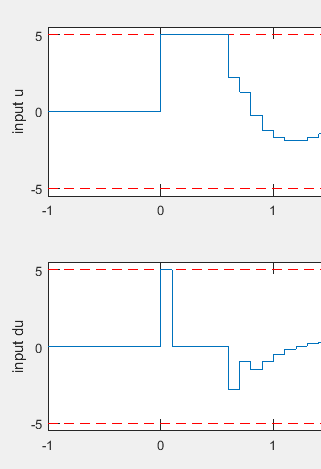
\includegraphics[width=0.7\linewidth]{11_nosteps.png}
\caption{Vypnuté obmedzenie.}
\label{11_nosteps}
\end{subfigure}
\caption{Ukážka vplyvu obmedzenia zmeny riadiaceho zásahu na časový priebeh riadiaceho zásahu.}
\end{figure}

\begin{itemize}
  \item \textbf{Obmedzenie veľkosti akčného zásahu} je možné pozorovať v strednom grafe obrázku \ref{09_out} pri zmene 2. v čase 5.3 sekundy, kedy vidieť ako systém narazil na obmedzenie akčného zásahu a na tejto hodnote ostane až do času 6.1 sekundy. Ak by obmedzenie nebolo samozrejme by bola doba regulácie kratšia avšak akčný zásah bez obmedzení vo väčšine prípadov nezodpovedá realite.
  \item \textbf{Obmedzenie veľkosti zmeny akčného zásahu} je opäť možné pozorovať v strednom grafe obrázku \ref{09_out} pri obidvoch zmenách referenčného signálu. Zvýraznené to je v obrázku \ref{10_steps}. Riadiaci zásah v~tvare ,,schodov`` je dôsledkom tohto obmedzenia zmeny akčného zásahu. Z obrázku \ref{10_steps} je možné vyčítať periódu vzorkovania 0.1 sekundy, keďže je v grafe za 1 sekundu 10 zmien akčného zásahu. Prípad, že obmedzenie zmeny akčného zásahu je nastavené na hodnotu 5 (rovnaká ako obmedzenie akčného zásahu) je zobrazené na obrázku \ref{11_nosteps}.
\end{itemize}   


Na základe týchto experimentov sa potvrdzujú výhody MPC regulátora, ktoré boli spomenuté v úvode ohľadne jednoduchosti zavedenia obmedzení. V tomto má MPC bližšie spojenie s reálnym systémom ako iné regulátory napr. PID, kde kvôli obmedzeniu akčného zásahu treba robiť doplňujúce úpravy tzv. antiwindup zapojenie PID regulátora. 

\subsubsection{Opis systému riadenia plynovej turbíny}
V tejto časti je overenie algoritmu na reálnom systéme z praxe, ktorý je tu popísaný. Následne je identifikovaný matematický model systému a overenie funkčnosti MPC princípov. Treba zdôrazniť, že overenie je stále prostredníctvom simulácie v prostredí Matlab.

\indent Turbína s~výkonom 1.5MW obsahuje tri hlavné časti, menovite, kompresor,
spaľovaciu komorou a~vysokotlakovú turbínu. V~rokoch 1950 bolo
priemyselné využitie turbín významne rozšírené, kvôli jej nespočetným
výhodám. Napríklad neprítomnosť častí, ktoré by sa o~seba odierali,
nízka spotreba palív a~vysoká operačná spoľahlivosť. Prvá časť turbíny
zahŕňa stláčanie vzduchu na poskytnutie vysokého pomeru tlaku medzi
turbínou a~kompresorom, takže sa vzduch rozpína do turbíny. Zvyšovanie
teploty vzduchu spaľovaním paliva spôsobuje väčšie rozpínanie horúceho
vzduchu v~turbíne, poskytujúc tak potrebný výstupný výkon. Pre rôzne
prietoky vzduchu je limitovaný pomer vzduchu, ktorý môže byť dodaný, čo
je označované ako pomer palivo/vzduch. Tento faktor obmedzuje výstupný
výkon, ktorý môže byť dosiahnutý.~Maximálny pomer palivo/vzduch je
určený pracovnou teplotou lopatiek turbíny, ktoré sú vysoko stláčané.
Zaznamenanie možnej poruchy lopatiek je dôležitý problém pri monitoringu
a~detekcii chýb. Primárna požiadavka na riadenie je výstupný výkon, ale
neexistuje žiadny vhodný spôsob merania výkonu. Premenné súvisiace
s~výkonom sú riadené prostredníctvom riadenia generátora rýchlosti
N\textsubscript{g}, moduláciou prívodu paliva, kde N\textsubscript{g} je
funkciou výkonu generátora. Riadiaci zásah určuje množstvo paliva
dodávaného do motora, čo je funkciou uhla otvorenia klapky
\(\theta_{v}.\) Parametre systému a~regulátora: rýchlosť
motora leží medzi 0 a~30~000 rpm (=500rps) táto premenná môže byť
považovaná za známu a~reprezentuje od 0 po 1.5MW. Vstup do systému je
náklon plynovej klapky 0-60°, čo je ekvivalent toku paliva 0-625kg/h.
Riadiaci rozsah výkonu je od 0 po plný výkon. Od 17~001-27~000 rpm
(283,35-450rps) je považovaný za stabilný stav rýchlosti generátora.\cite{MPC07}
\subsubsection{Identifikácia a riadenie systému plynovej turbíny}
Vstupné dáta na identifikáciu systému po posunutí do 0 sú zobrazené na obrázku  \ref{12_data}. 

\begin{figure}[!htbp]
\centering
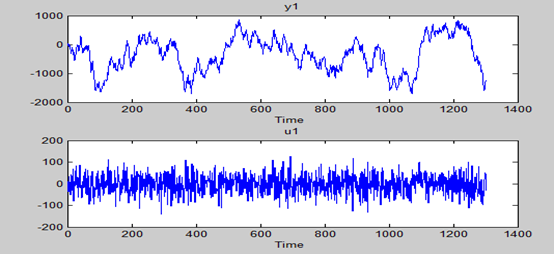
\includegraphics[width=0.9\textwidth]{12_data.png}
\caption{Časový priebeh nameraných údajov výstup a vstup systému.}
\label{12_data}
\end{figure}
Premenná y\textsubscript{1} reprezentuje výstup - otáčky motora a~u\textsubscript{1}
vstup systému - natočenie klapky. Na identifikáciu systému bol použitý Matlab nástroj \textit{ident}. Pri zisťovaní matematického modelu bolo vyskúšaných viacero metód. Najlepšie
výsledky - percento zhody nameraných a simulovaných dát dal arx model. Porovnanie nameraných a~simulovaných dát sú na
obrázku \ref{13_ident}.


\begin{figure}[!htbp]
\centering
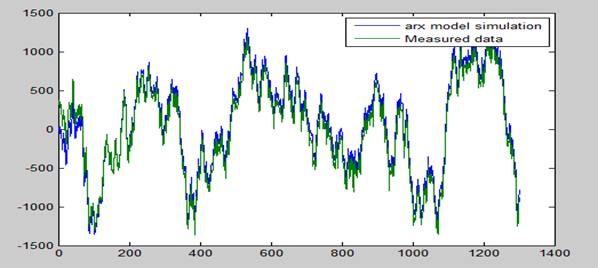
\includegraphics[width=0.9\textwidth]{13_ident.png}
\caption{Porovnanie simulovaných a nameraných údajov}
\label{13_ident}
\end{figure}
Os x predstavuje čas v sekundách a y predstavuje výstup systému. Pomocou modelu arx sa získala nasledovná prenosová funkcia

\begin{equation} \label{eq38}
\begin{split}
Gp(z) = \ \frac{Y(z)}{U(z)}
\end{split}
\end{equation}

kde
\begin{equation} \label{eq39}
\begin{split}
\text{\ Y}\left( z \right) = 2.085z^{- 1} + 0.3692z^{- 2} \\
U\left( z \right) = 1 - 0.99{13z}^{- 1} + 1.287 \times 10^{- 3}z^{- 2}
\end{split}
\end{equation}
Perióda vzorkovania je \(T_{s} = 0.25\).

Navrhnutý algoritmus bol otestovaný na reálnom systéme s~prenosovou
funkciou \ref{eq39}. Parametre simulácie sú zobrazene na obrázku \ref{15_paramt}. Časové odozvy systému s~MPC regulátorom sú
na obrázku \ref{14_simt}. Konkrétne časová odozva výstupu, v~tomto prípade
výkon motora, meraný v~rps (otáčky za sekundu) je zobrazený vo vrchnom
grafe. Vstup systému, uhol náklonu plynovej klapky meraný v~stupňoch je
v~strednom grafe a~zmena vstupu v~spodnom grafe. Všetky spomenuté
veličiny majú v~grafe modrú farbu. Zelená farba vo vrchnom grafe
predstavuje referenčný signál a~červené čiarkované čiary sú obmedzenia.

\begin{figure}[!htbp]
\centering
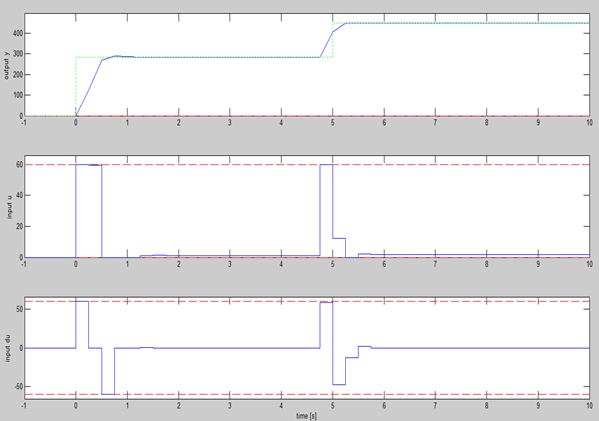
\includegraphics[width=0.9\textwidth]{14_simt.png}
\caption{Časové odozvy rýchlosti motora (v jednotkách rps) s MPC regulátorom}
\label{14_simt}
\end{figure}

\begin{figure}[!htbp]
\centering
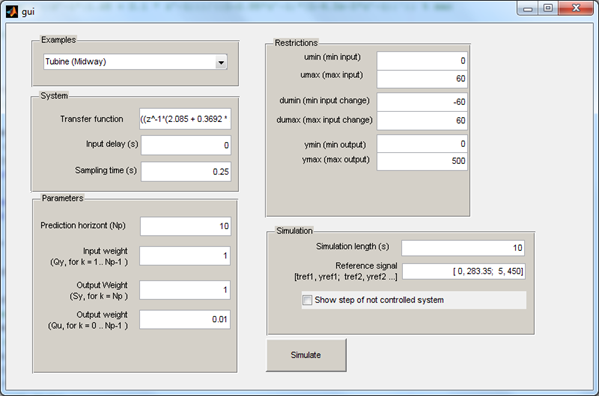
\includegraphics[width=0.9\textwidth]{15_paramt.png}
\caption{Parametre simulácie}
\label{15_paramt}
\end{figure}

Prenosová funkcia (\ref{eq39}) sa zadala do grafického rozhrania do pola
„transfer function``. Horizont predikcie bol nastavený na 10 vzoriek
dopredu. Zo simulácii vyplýva, že je to dostatočné a~efektívne, berúc do
úvahy odozvu systému a~kvalitu riadenia. Váhy boli nastavené na
prednastavené hodnoty. Obmedzenia algoritmu sú

\begin{itemize}
\item
  Na vstup 0-60 stupňov.
\item
  Zmena vstupu -60 -- 60 stupňov.
\item
  Výstup systému 0 -- 500 rps (30~000 rpm)
\end{itemize}

Referenčný signál je nastavený na hodnotu 283.35 rps v~čase 0. Po 5
sekundách je nastavený na hodnotu 450 rps.

Z~výsledkov je možné vidieť výhody prediktívneho riadenia. Keďže
prediktívny regulátor je založený na optimalizácii, je možné vidieť
minimálne akčné zásahy, čo môže viesť k~úspore spotreby.\cite{MPC08}\\
Týmto končí simulačné overovanie algoritmu MPC regulátora vytvoreného na základe teoretických princípov popísaných v úvodných kapitolách MPC regulátora a nasleduje druhá časť práce, ktorá pripraví podklady pre  praktický experiment, ktorý okrem iného zahŕňa definíciu IoT a niekoľko ďalších pojmov z oblasti softvérovej architektúry.

\section{Softvérové architektúry pre pokročilé metódy riadenia}
Téma softvérovej architektúry (Software architectrue) zahŕňa veľa súčastí. Moderne metódy a algoritmy riadenia vyžadujú využívanie najnovších poznatkov v oblasti IT za účelom zvýšenia kvality, rýchlosti riešení a dosiahnutia vysokej bezpečnosti a spoľahlivosti systému. Jednou z najdôležitejších úloh v oblasti využívania moderných metód riadenia je využitie pokročilých informačných technológii s optimálnou štruktúrou, čím sa zaoberá práve softvérová architektúra. Pri návrhu regulátora do praxe nie je dôležitý len samotný algoritmus regulátora, ale celé jeho zavedenie do procesu. V súčasnej dobe dochádza k užšej spätosti IT a OT, preto je nevyhnutné pri návrhu regulátora mať aj znalosti o prostredí, v ktorom regulátor má spoľahlivo fungovať. Práca sa preto v druhej časti zameriava na oblasť softvérovej architektúry. A hlavne tých oblastí, ktoré vedú do problematiky internetu vecí a zároveň súvisia s aplikáciou pokročilých metód riadenia v praxi. Nasleduje niekoľko definícií softvérovej architektúry na neskoršie pochopenie toho, aké výzvy prináša užšia väzba medzi IT (informačnými technológiami) a OT (operačnými technológiami) a aké znalosti sú nevyhnutné pri návrhu prostredia pre regulátor.

\indent Softvérová architektúra je proces definovania štrukturovaného riešenia, ktoré spĺňa všetky technické a operačné požiadavky, zatiaľ čo optimalizuje bežné kvalitatívne vlastnosti ako je výkonnosť, bezpečnosť a ovládateľnosť. Zahŕňa rad rozhodnutí, ktoré sú založené na viacerých faktoroch a každé z týchto rozhodnutí môže mať značný dopad na kvalitu, výkonnosť, udržiavanie a celkový úspech aplikácie.

\indent Philippe Kruchten, Grady Booch, Kurt Bittner a Rich Reitman odvodili a vylepšili definíciu architektúry, ktorá vychádza z práce Mary Shaw a David Garlan (Shaw and Garlan 1996). Ich definícia je:

\indent Softvérová architektúra zahŕňa sadu dôležitých rozhodnutí o usporiadaní softvérového systému vrátane voľby stavebných prvkov a ich rozhraní, pomocou ktorých je systém zložený. Rozhodnutie o voľbe správania, ktoré je definované spoluprácou medzi uvedenými prvkami. Rozhodnutie o spájaní týchto štrukturálnych a behaviorálnych elementov do rozsiahlejších subsystémov a voľba architektonického štýlu, ktorý vedie toto usporiadanie. Softvérová architektúra tiež zahŕňa starosť o funkcionalitu, použiteľnosť, pružnosť, výkonnosť, možnosť znovu použitia, zrozumiteľnosť, kompromisy na ekonomické a technologické obmedzenia a tiež estetickosť. \cite{IOT02}

\indent Dôležité si je uvedomiť, že softvérová architektúra je prostriedok na vytvorenie softvérového systému avšak softvérový systém je stále len prostriedok na dosiahnutie určitého cieľa v našom prípade vytvorenie softvérového prostredia pre aplikovanie moderných metód riadenia.

\indent Preto by systémy mali byť navrhované s prihliadaním na \textbf{používateľa}, \textbf{systém} (IT infraštruktúra) a \textbf{biznis ciele}, ako je zobrazené na obrázku \ref{18_arch}. Pre každú z týchto oblastí by mal byť načrtnutý kľúčový scenár a identifikované dôležité kvalitatívne vlastnosti (napríklad spoľahlivosť a škálovateľnosť) a kľúčové oblasti uspokojenia alebo neuspokojenia. Vytvoriť metriky a prihliadať na ne pri meraní úspechu v každej z oblasti, všade kde je to možné.\cite{IOT02}
\begin{figure}[!htbp]
\centering
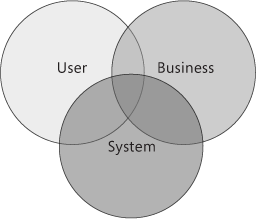
\includegraphics[width=0.3\textwidth]{18_arch.png}
\caption{Oblasti, potrebné zvažovať pri návrhu\cite{IOT02}}
\label{18_arch}
\end{figure}
V oblasti riadenia sú prioritné biznis ciele kvalita regulácie, jej dosiahnutie  a udržiavanie. Tiež platí, že je potrebné si nastaviť miery kvality regulácie a teda škálu od akceptovateľných až po neakceptovateľné ukazovatele. Všeobecné definície zdôraznili kľúčové oblasti, ktoré treba mať na pamäti pri návrhu softvérového systému v našom prípade pre proces riadiacu aplikáciu, avšak definície zatiaľ nepomohli s návrhom samotným, preto nasleduje vymenovanie základných typov architektúr, z ktorých si je pri návrhu možné voliť.

\subsection{Základne typy architektúr}
Jedno z kľúčových rozhodnutí je voľba typu architektúry. Tie najpoužívanejšie sú vymenované nižšie podľa článku \cite{IOT05} napísanom na základe knihy\cite{IOT08}, ktorú napísal Mark Richards - softvér architekt s 30 ročnou skúsenosťou. V článku sa tiež uvádza, že v jednom systéme môže byť použitých viacero typov, čo je  dôležitá informácia pri návrhu.
\begin{itemize}
 \item \textbf{ N-vrstvová architektúra.} Je to jeden z najpoužívanejších prístupov, pretože je to postavené okolo databázy a veľa aplikácií v biznise prirodzene potrebujú ukladať informácie v tabuľkách. \indent Veľa z najznámejších frameworkov ako Java EE, Drupal a Express sú postavené tak, aby mali túto štruktúru na mysli, takže aplikácie, nimi vytvorené sú automaticky N-vrstvové.
\indent Zdrojový kód je usporiadaný tak, že dáta vstupujú na najvyššej úrovni a prepracujú sa cez každú vrstvu až dosiahnú najnižšiu, čo je zvyčajne databáza. Po ceste má každá vrstva svoju úlohu, ako kontrolovanie konzistencie dát alebo formátovanie dát, tak aby ostali konzistentné. Je bežné, že rôzny programátori pracujú nezávisle na jednotlivých vrstvách.
\begin{figure}[!htbp]
\centering
\begin{subfigure}{0.5\linewidth}
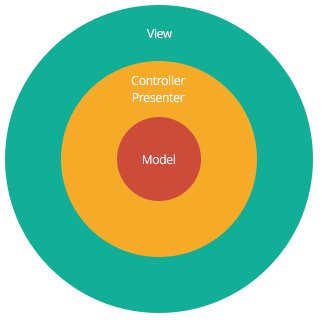
\includegraphics[width=0.9\textwidth]{25_3l.png}
\caption{3 vrstvová architektúra \cite{IOT07}}
\label{25_3l}
\end{subfigure}%
\begin{subfigure}{0.5\linewidth}
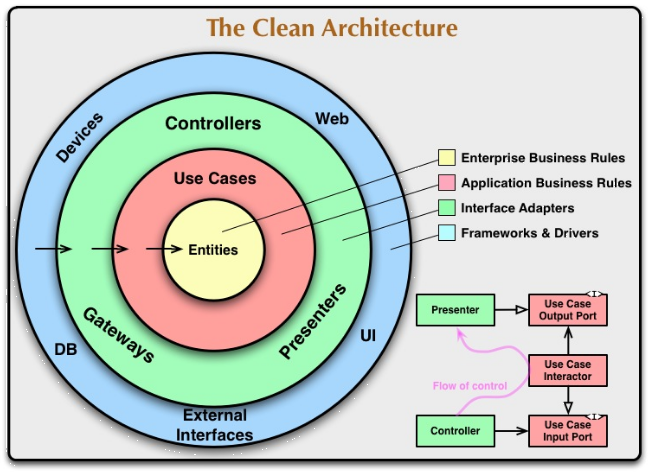
\includegraphics[width=0.9\textwidth]{24_4l.png}
\caption{4 vrstvová architektúra\cite{IOT06}}
\label{24_4l}
\end{subfigure}
\caption{Rôzne počty vrstiev architektúry.}
\end{figure}
MVC (Model-View-Controller) štruktúra, ktorú poskytuje väčšina obľúbených frameworkov je zjavne N-vrstvová architektúra. Nad databázou je model, ktorý často obsahuje biznis logiku a informácie o type dát databáze. Na vrchu je zobrazovacia vrstva, ktorá často pozostáva z CSS, JavaScript a HTML. V strede je ovládač, ktorý má viacero pravidiel a funkcií na transformáciu dát zo zobrazovacej vrstvy do modelu.
 \item \textbf{ Architektúra riadená udalosťami.} Veľa programov trávi väčšinu času čakaním, kým sa niečo stane. Tento fakt špeciálne platí pre systémy, ktoré priamo spolupracujú  s ľuďmi, ale rovnako je to bežné aj v oblasti sietí.
\indent Architektúra riadená udalosťami pomáha spravovať uvedené fakty tak, že sa vytvorí centrálna jednotka, ktorá prijíma dáta a potom ich deleguje do samostatných modulov, ktoré dáta spracujú. Toto odovzdanie sa nazýva vygenerovanie udalosti. Udalosť je následne spracovaná kódom tzv. event-handler.
 \item \textbf{ ,,Microkernel`` architektúra.} Veľa aplikácií má základnú sadu operácií, ktoré sú znova a znova použité v iných prípadoch, ktoré závisia od aktuálneho typu dát a typu úlohy. Obľúbený nástroj na vývoj Eclipse, napríklad, najskôr otvorí súbory, pridá im poznámky, upraví ich a potom spustí pomocníka na pozadí. Nástroj je vykonávaním týchto operácií známy a s kódom napísaným v jazyku Java na jedno stlačenie tlačítka sa kód skompiluje a spustí.
\indent V tomto prípade, základný program na zobrazovanie a upravovanie súboru sú súčasťou microkernel-u. Java kompilátor je extra časť, ktorá je pridaná na podporu základných čŕt microkernel-u. Ostatní vývojári vyvinuli ďalšie časti, aby bolo možné vyvíjať aj v iných jazykoch s inými kompilátormi. Často krát sa kompilátor ani nepoužíva, ale využívajú len funkcie na úpravu súborov. 
\indent Špeciálne pridaná funkcionalita sa nazýva plug-in. Často je tento prístup nazývaný aj Plug-in architektúra.
 \item \textbf{ ,,Microservice`` architektúra.} Softvér môže byť ako malý slon. Keď je malý je milý a zábavný, ale keď dospeje, je ťažké ho viesť a bráni sa zmene. Návrh Microservice architektúry pomáha vývojárom predísť tomu, aby sa z ich malých programov stali ťažkopádne, monolitické a neflexibilné programy. Preto na miesto vytvárania jedného veľkého programu je cieľ vytvoriť množstvo rozličných malých programov a vždy keď chce niekto pridať funkcionalitu, tak vždy pridať malý program.
\indent Tento prístup je podobný Microkernel 
a udalosťami riadenému prístupu, ale je používaný zvyčajne, keď rozličné úlohy sú ľahko oddeliteľné. Vo veľa prípadoch, rozličné úlohy môžu vyžadovať rôzny čas na spracovanie a môžu sa líšiť v spôsobe použitia. Napríklad servery spoločnosti Netflix, ktoré poskytujú obsah zákazníkom (filmy a videá) majú oveľa väčšiu záťaž v piatok a sobotu večer, takže musia byť pripravený zvýšiť výpočtové a sieťové kapacity. Servery, ktoré sledujú vrátenie požičaných DVD, na druhej strane, robia svoju robotu cez týždeň hneď ako pošta doručí príchodzie zásielky. Ak sa to implementuje ako oddelené služby, Netflix cloud ich môže nezávisle škálovať podľa dopytu.
 \item \textbf{ ,,Space-based`` architektúra.} Veľa aplikácií, ktoré sú postavené okolo databázy a fungujú správne pokiaľ databáza stíha spracovávať záťaž. Keď však databáza prestane stíhať zapisovať veľa transakcií, celá aplikácia spadne.
 \indent ,,Space-based`` architektúra je navrhnutá tak, aby predišla zlyhaniu pri veľkej záťaži rozložením spracovania a ukladania na viacero serverov. Dáta aj zodpovednosť za možnosť zavolania služby sú rozdistribuované na viacero uzlov. Niektorí architekti používajú širokejší pojem ,,cloud`` architektúra. Táto architektúra podporuje prípady, kedy je ťažké predikovať nárast požiadaviek, ktorý by databáza nestíhala spracovávať. 
\indent Uchovávanie informácie v RAM umožňuje vykonávať veľa úloh rýchlejšie a zjednodušuje zdieľanie medzi uzlami. Avšak distribuovaná architektúra robí niektoré analýzy komplikovanejšími. Výpočet, ktorý musí prebehnúť cez všetky dáta, napríklad výpočet priemeru alebo vytváranie štatistickej analýzy musí byť rozdelený na podúlohy cez všetky uzly a keď skončia zoskupenie dát je potrebné. 
\end{itemize}

\subsection{Základné typy aplikácií}
Ďalšie z kľúčových rozhodnutí je voľba typu aplikácie. Na výber podľa  článku \cite{IOT03} sú:
\begin{itemize}
\item
 \textbf{Mobilná aplikácia obrázok \ref{19_mob}.} Aplikácie tohto typu môžu byť vyvíjané ako tenký alebo tučný klient. Mobilná aplikácia vo forme tučného klienta môže podporovať scenáre bez pripojenia alebo s občasným pripojením. Webové aplikácie alebo tenkí klienti podporujú iba scenáre s pripojením. Zdroje, ktorými disponujú mobilné zariadenia sa často ukazujú ako obmedzenie pri návrhu mobilných aplikácií. \\
Výhody: 
 \begin{itemize}
   \item  Podpora mobilných zariadení.
   \item  Dostupnosť a jednoduchosť použitia pre používateľov mimo kancelárie.
   \item  Podpora pre scenáre bez pripojenia a s občasným pripojením.   
 \end{itemize}
Na zváženie: 
 \begin{itemize}
   \item Limity ohľadne zadávania údajov a navigácie v aplikácii.
   \item Limitovaná šírka zobrazovanej plochy.   
 \end{itemize}
 
\item
 \textbf{Tučná klientská aplikácia obrázok \ref{20_cli}.} Aplikácie tohto typu sú zvyčajne vyvíjané ako stand-alone aplikácie s grafickým rozhraním, ktoré zobrazuje dáta prostredníctvom rôznych ovládacích prvkov. Tuční klienti sú väčšinou navrhnutí na scenáre bez pripojenia alebo s občasným pripojením, keď potrebujú prístup k vzdialeným dátam alebo funkcionalite. \\
Výhody: 
 \begin{itemize}
   \item  Možnosť využívať zdroje klienta.
   \item  Lepšia odozva, bohatá funkčnosť používateľského rozhrania a lepší používateľský zážitok.
   \item  Dynamická a responzívna interakcia.
   \item Podpora scenárov bez pripojenia alebo s dočasným pripojením.   
 \end{itemize}
Na zváženie: 
 \begin{itemize}
   \item Komplikovanejšie nasadenie. Avšak existuje množstvo dostupných inštalačných možnosti ako ClickOnce, Windows Installer a XCOPY.
   \item Problém s nasadzovaním nových verzií v čase.   
   \item Závislé od platformy.
 \end{itemize}


\begin{figure}[!htbp]
\centering
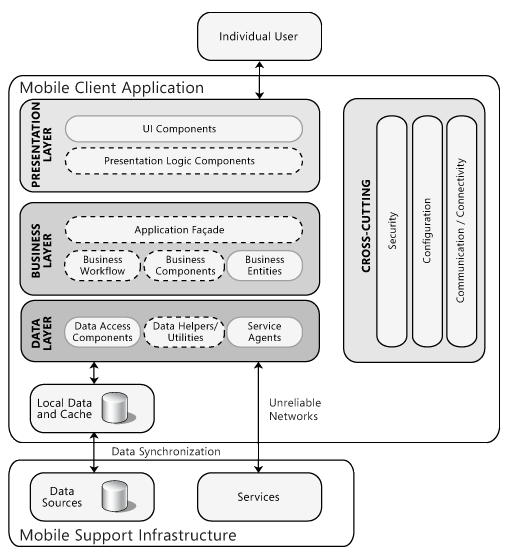
\includegraphics[width=0.9\textwidth]{19_mob.png}
\caption{Mobilná aplikácia \cite{IOT03}}
\label{19_mob}
\end{figure}

\begin{figure}[!htbp]
\centering
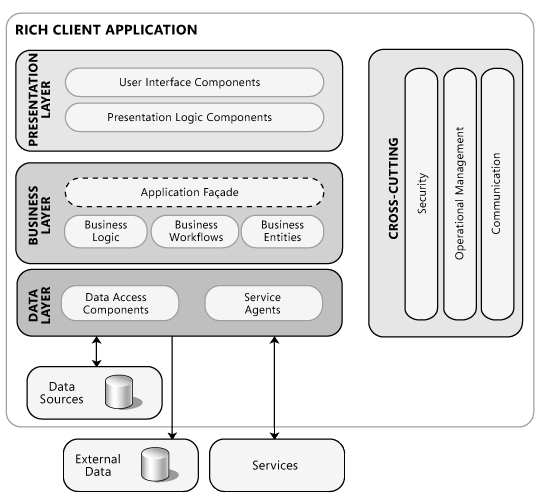
\includegraphics[width=0.9\textwidth]{20_cli.png}
\caption{Clientská aplikácia \cite{IOT03}}
\label{20_cli}
\end{figure}
 
\item
 \textbf{Tučná internetová aplikácia obrázok \ref{21_ri}.} Aplikácie tohto typu sú vyvíjané tak, aby podporovali viacero platforiem a prehliadačov tak, že zobrazujú multimédia alebo iný grafický obsah. Tučné internetové aplikácie bežia v prehliadači, čím sú obmedzené pristupovať k niektorým zdrojom klienta. \\
Výhody: 
 \begin{itemize}
   \item  Rovnaké schopnosti užívateľského rozhrania ako tuční klienti.
   \item  Podpora multimédií a stream medií
   \item  Jednoduché nasadzovanie  s rovnakými možnosťami distribúcie ako weboví klienti. 
   \item Jednoduchý upgrade na novú verziu.
   \item Podpora cez väčšinu platforiem a prehliadačov. 
 \end{itemize}
Na zváženie: 
 \begin{itemize}
   \item Kladie vyššie nároky na klienta ako webové aplikácie.
   \item Obmedzenia na využívanie zdrojov klienta oproti tučnej klientskej aplikácii. 
   \item Vyžaduje mať na klientovi nasadený vhodný runtime framework.
 \end{itemize} 
 
  \item
  \textbf{Webová aplikácia obrázok \ref{23_web}.} Aplikácie tohoto typu zvyčajne podporujú scenáre s pripojením, podporujú viacero prehliadačov, ktoré bežia na rôznych operačných systémoch.\\
Výhody: 
 \begin{itemize}
   \item Široká dostupnosť pre väčšinu platforiem a užívateľské rozhranie je vytvárané prostredníctvom štandardov.
   \item Jednoduchosť nasadenia a správy zmien.
 \end{itemize}
Na zváženie: 
 \begin{itemize}
   \item Závislé od nepretržitého sieťového spojenia.
   \item Komplikácie s poskytnutím bohatého (rich) užívateľského rozhrania.
 \end{itemize}  
 
\begin{figure}[!htbp]
\centering
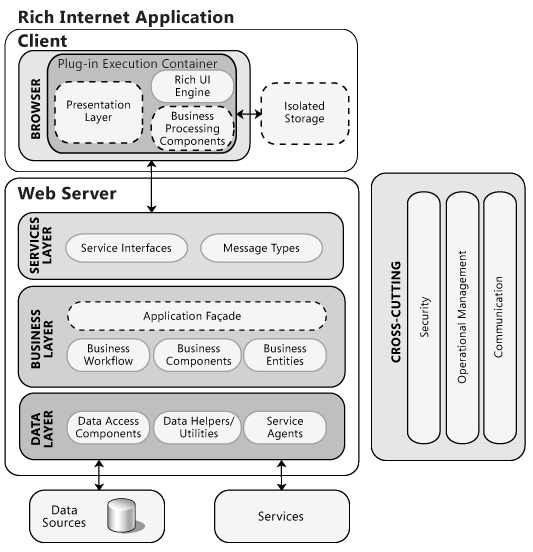
\includegraphics[width=0.9\textwidth]{21_ri.png}
\caption{Tučná internet aplikácia \cite{IOT03}}
\label{21_ri}
\end{figure}

\begin{figure}[!htbp]
\centering
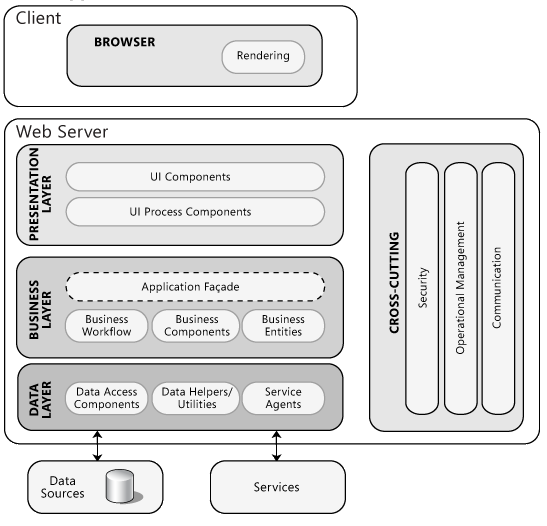
\includegraphics[width=0.9\textwidth]{23_web.png}
\caption{Web aplikácia \cite{IOT03}}
\label{23_web}
\end{figure}

 \item
  \textbf{Servisná aplikácia obrázok \ref{22_ser}.} Služby vystavujú zdieľanú biznis funkcionalitu a umožňujú klientom pristupovať k nim z lokálneho alebo vzdialeného systému. Operácie služieb sú volané prostredníctvom správ založených na XML schémach, posielaných cez transportnú vrstvu. Cieľom týchto aplikácií je dosiahnutie voľných väzieb medzi klientom a serverom. \\
Výhody: 
 \begin{itemize}
   \item Interakcie medzi klientom a serverom je prostredníctvom voľných väzieb.
   \item Môže byť použitá rôznymi nezávislými aplikáciami.
   \item Podpora pre interoperabilitu.
 \end{itemize}
Na zváženie: 
 \begin{itemize}
   \item Nie je podpora pomocou užívateľského rozhrania.
   \item Závisí od sieťového pripojenia.
 \end{itemize} 

\begin{figure}[!htbp]
\centering
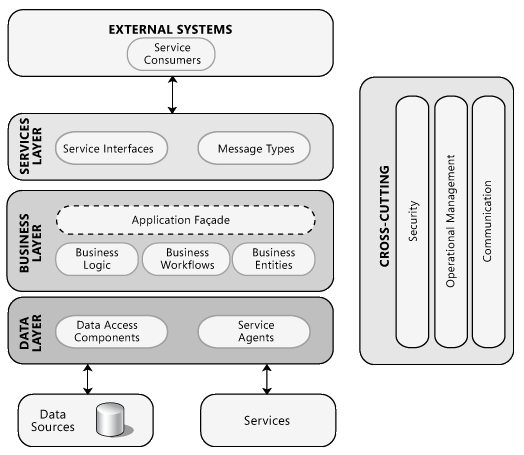
\includegraphics[width=0.75\textwidth]{22_ser.png}
\caption{Aplikácia poskytujúca službu \cite{IOT03}}
\label{22_ser}
\end{figure} 
    
\end{itemize}
\subsubsection{Servisná aplikácia}
Servisným aplikáciam je v práci venovaná samostatná kapitola, pretože je to najvhodnejší spôsob akým moderné metódy riadenia, či už jeden alebo viac regulátorov integrovať do softvérového systému. Servisné aplikácie majú svoje miesto vo väčšine enterprise architektúr.  Enterprise architektúra je koncepčný návrh, ktorý definuje štruktúru a prevádzkovanie spoločnosti.\\ 
\indent Zámer enterprise architektúry je rozhodnúť ako môže organizácia najefektívnejšie dosiahnuť aktuálne a budúce ciele \cite{IOT09}. Inými slovami ide o  architektúru podnikových informačných systémov, ktoré zvyčajne pozostávajú z viacerých súčasti. Príkladom týchto súčasti môže byť:
\begin{itemize}
  \item  \textbf{CRM aplikácia.} Podľa APICS slovníka \cite{IOT10} je CRM definované ako úložisko a analýza informácií navrhované pre podporu predajných a marketingových rozhodnutí, na pochopenie a podporu potrieb existujúcich a potenciálnych zákazníkov. Zahŕňa správu užívateľských účtov, môže zahŕňať katalóg produktov, zadávanie objednávky, spracovanie a úpravu platieb a iné funkcie.\cite{IOT11}. Všetky, ktoré sú v definícii uvedené ako ,,môže zahŕňať``, závisí od konkrétnej implementácie, či dané funkcionality CRM obsahuje alebo nie. Pretože každá zo spomenutých funkcionalít môže byť ako samostatná servisná aplikácia. V tejto práci sú uvedené ako samostatné časti a CRM sa tu obmedzí na správu užívateľských účtov.
  \item  \textbf{Katalóg produktov.} Na manažovanie závislosti medzi produktami a ovplyvňovanie typov zliav a teda výpočet ceny za produkty býva v podnikoch samostatná aplikácia
 \item  \textbf{Účtovná aplikácia.} Aplikácia na vedenie účtovníctva
 \item  \textbf{Správa majetku.} Aplikácia na správu majetku. 
  \item  \textbf{ERP aplikácia.} (Plánovanie zdrojov v podniku je pojem používaný v priemysle pre širokú škálu činností, ktoré pomáhajú organizácii spravovať jej biznis. Dôležitý cieľ je pomôcť, aby tok informácií bol nastavený tak, že biznis rozhodnutia môžu byť robené na základe poskytnutých dát. ERP aplikácie sú robené tak, aby zbierali a zatrieďovali dáta z rôznych úrovni organizácie a poskytovali tak manažmentu náhľad na kľúčové ukazovatele výkonnosti tzv. KPIs v reálnom čase.\cite{IOT12} 
\end{itemize} 
Súčastí môže byť samozrejme viac a každá organizácia si podľa svojich potrieb vyberá tie  súčasti, ktoré potrebuje. Väčšina spomenutých súčasti je dodávaná ako servisná aplikácia. Aplikácie medzi sebou môžu komunikovať prostredníctvom vystavených rozhraní. Pri malom počte vystavených rozhraní sa často používa \textbf{Point to Point \ref{26_p2p}} architektúra, kedy neexistuje centrálny bod vystavenia služby, ale ak ktorákoľvek aplikácia potrebuje zavolať inú, tak ju priamo zavolá. Takýto prístup je však krátkozraký, lebo prax ukazuje, že počet vystavených služieb časom vždy pribúda, preto je dnes rozšírené použivať tzv. SOA - \textbf{Service oriented architektúru \ref{27_soa}}, čo je iný názov spomínanej ,,Microservice`` architektúry s centrálnym bodom vystavovania služieb tzv. ESB - Enterprise service bus.
\begin{figure}[!htbp]
\centering
\begin{subfigure}{0.5\linewidth}
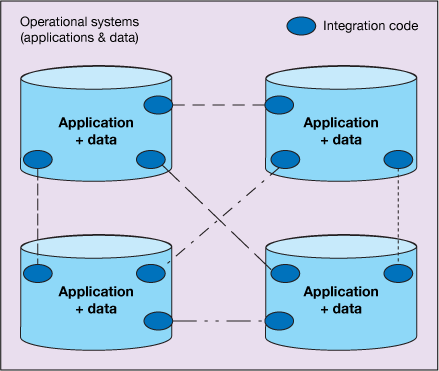
\includegraphics[width=0.8\textwidth]{26_p2p.png}
\caption{Point to Point \cite{IOT13}}
\label{26_p2p}
\end{subfigure}%
\begin{subfigure}{0.5\linewidth}
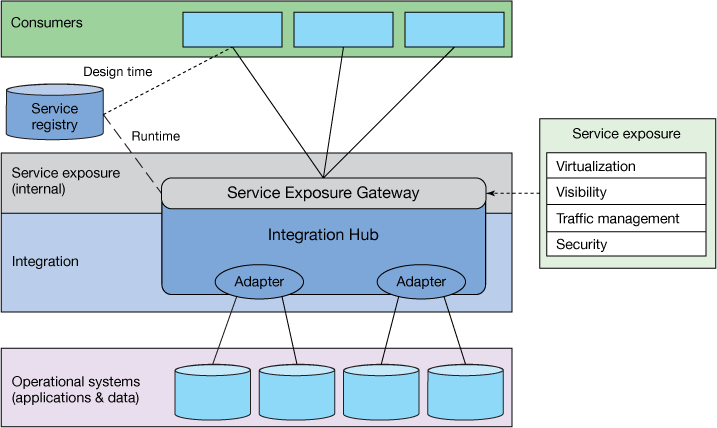
\includegraphics[width=1.1\textwidth]{27_soa.png}
\caption{SOA \cite{IOT13}}
\label{27_soa}
\end{subfigure}
\caption{Porovnanie architektúr.}
\end{figure}
Existuje viacero spôsobov ako SOA implementovať. 
\begin{itemize}
 \item Najznámejší spôsob implementácie SOA, ktorí dnes používa väčšina užívateľov informačných technológií je implementácia protokolu WWW - \textbf{World Wide Web} v skratke často označovaný len WEB. 
\begin{figure}[!htbp]
\centering

\includegraphics[width=0.75\textwidth]{28_web.png}
\caption{WWW \cite{IOT14}}
\label{28_web}
\end{figure} 
Obrázok \ref{28_web} znázorňuje princíp fungovania. Prehliadač (web browser) je v pozícii klienta, konzumera služby, ktorú poskytuje Web Server. Web Server je označenie takého počítača, na ktorom beží servisná aplikácia, ktorá vie na základe definovaných pravidiel poskytnúť požadovaný obsah. Najpoužívanejšie aplikácie, ktoré z počítača spravia web server,  v čase písania práce, z prieskumu robenom vo februári 2016 \cite{IOT15} sú Apache, Nginx, Microsoft IIS. Ich preferencie striedavo kolíšu podľa úspechu najnovších verzií. Pod službou sa v tomto prípade rozumie poskytnutie HTML dokumentu prostredníctvom aplikačného komunikačného protokolu HTTP.
\item Ďalší rozšírený protokol, ktorý implementuje SOA architektúru je \textbf{protokol SOAP}. Princíp fungovania je na obrázku \ref{29_soap}.
\begin{figure}[!htbp]
\centering
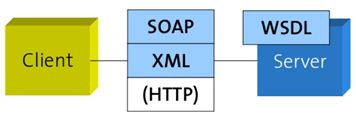
\includegraphics[width=0.75\textwidth]{29_soap.png}
\caption{SOAP \cite{IOT14}}
\label{29_soap}
\end{figure} 
Klient je v tomto prípade generickejší. Zvyčajne je to aplikácia, ktorá má XML parser (prekladač) a schopnosť komunikovať po sieti HTTP protokolom. Rovnako server je generickejší. SOAP je v tomto prípade pre server ,,len`` príručka ako službu vystaviť. Pod službou sa rozumie vystavenie RPC (remote procedure call), čo znamená umožnenie volania vzdialenej procedúry. Čo bude procedúra robiť je plne v rukách programátora. Aj v SOAP je pre transportnú vrstvu použitý HTTP protokol, obsahom správ sú XML objekty so špecifickým tvarom, ktorý SOAP definuje. Postup komunikácie je taký, že klient vytvorí XML objekt v ktorom definuje vstupné parametre do volania vzdialenej procedúry odošle požiadavku, na serveri sa vykoná procedúra a do odpovede sa pošle výsledok spracovania vzdialenej procedúry vo forme XML objektu, ktorý klient spracuje a na základe toho vie ako volanie dopadlo. 
Medzi najväčšie výhody tohto protokolu patrí možnosť striktnej validácie správnosti formátu správ, ktoré si klient a server vymieňajú. Formát správ a operácie, ktoré server poskytuje sú zadefinované vo WSDL dokumente. 
 \item Iná implementácia SOA architektúry uvádzaná v tejto práci je \textbf{architektonický štýl REST}. Možností samozrejme existuje viacero, ale ako bolo na začiatku tejto kapitoly uvedené, cieľom je pripraviť podklad pre vysvetlenie Internetu vecí a pre implementáciu MPC v ňom. REST je skratka od REpresentational State Transfer. Ako je možné vidieť na obrázku \ref{30_rest} aj tu vystupuje generický klient a generický server ako v prípade SOAP protokolu.
\begin{figure}[!htbp]
\centering
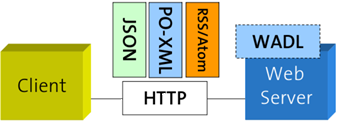
\includegraphics[width=0.75\textwidth]{30_rest.png}
\caption{REST \cite{IOT14}}
\label{30_rest}
\end{figure} 
Základný rozdiel oproti SOAP je, že HTTP je využívaný nie len ako transportný protokol, ale ako aplikačný protokol, takže sa využíva celý jeho potenciál. V praxi to znamená, že operácie, ktoré server poskytuje sú unifikované HTTP protokolom a nie je nutné, aby ich klient vyťahoval z WSDL dokumentu. Ďalšia výhoda, že HTTP je využívaný ako aplikačný protokol je, možnosť definovania aký obsah server pošle. Nie je teda obmedzenie na XML dokumenty, ale je možnosť posielať JSON objekty, binárne objekty a všetky ostatné typy správ podporované HTTP protokolom. Z uvedeného tiež vyplýva, že klientom môže byť samotný prehliadač respektíve implementácia klienta sa značne zjednodušuje. Možnosť posielať JSON objekty tiež napomáha zjednodušeniu klienta, ktorý, ak sa hovorí o web aplikácii, je zvyčajne napísaný v jazyku Javascript. Takže preklad posielanej správy na dátový typ klienta je priamočiary, bez používania ďalšieho prekladača. 
\end{itemize}
Kvôli uvedeným vlastnostiam je používanie REST rozhrania s JSON objektom ako formátom správ rozšírené pri tvorbe servisnej aplikácie, ktorá poskytuje rozhranie pre webovú aplikáciu.

\indent Fakty ohľadne enterprise architektúry, SOA architektúry a REST princípov, na prvý pohľad nesúvisiace s témou boli volené zámerne. Okrem toho, že trend aktuálnych IT systémov, je stavať ich v duchu uvedených faktov, tak aj zavádzanie moderných metód riadenia sa javí ako najoptimálnejšie týmto spôsobom, a teda pripájanie modulov (služieb) do systému, prostredníctvom REST princípov. Enterprise architektúra je navyše spomínaná z dôvodu toho, že zavedenie moderných metód riadenia nebude len pripojenie do jednoduchého systém, ale často veľkých podnikových IT prostredí. Posledný dôvod uvádzania týchto faktov je práve využívanie servisných aplikácií v IoT prostredí. Definíciou IoT pokračujeme v nasledujúcej kapitole.

\subsection{Internet vecí - IoT}
Organizácia IEEE vydala celý dokument  s názvom ,,Smerom k definícii Internetu vecí``. Cieľom dokumentu je podať plnohodnotnú definíciu IoT v rozmedzí od malých lokálnych systémov, obmedzených na konkrétnu lokalitu, až po globálny systém, ktorý je distribuovaný a poskladaný z komplexných systémov. V dokumente je možnosť nájsť prehľad základných požiadaviek na architektúru IoT \cite{IOT16}.
Podľa spoločnosti Gartner, ktorá je svetový líder v oblasti výskumu informačných technológií je IoT sieť fyzických objektov, ktoré majú vstavanú technológiu na komunikovanie a snímanie alebo interakciu s ich vnútornými stavmi alebo vonkajším prostredím \cite{IOT17}. 
Ešte definícia podľa stránky Techopedia: IoT je koncept, ktorý popisuje budúcnosť, kde každodenné fyzické objekty budú pripojené do internetu a budú sa vedieť sami identifikovať iným zariadeniam. Pojem je úzko spojený s RFID technológiou ako spôsobom komunikácie, aj keď to môže zahŕňať iné technológie na snímanie, bezdrôtové technológie alebo QR kódy.\\
\indent IoT je významné, pretože ak objekt sa vie sám digitálne reprezentovať stáva sa z neho niečo viac ako objekt samotný. Objekt sa už nevzťahuje len na nás, ale je spojený s okolitými objektami a dátami v databázach. Keď veľa objektov spolupracuje, je možné to nazvať ako inteligencia okolitého prostredia ,,ambient intelligence`` \cite{IOT18}.
Viacero ďalších technologických spoločností majú ich definíciu. Cieľom tejto práce nie je vytvoriť ďalšiu definíciu, ale identifikovať spoločné črty väčšiny definícií, ale hlavne načrtnúť možnosti zavedenia moderných metód riadenia do praxe. 
\begin{itemize}
 \item Prvá základná črta definícii je, že v nej vystupujú objekty, ktoré môžu \textbf{snímať a ovplyvňovať okolie}. Na dosiahnutie tejto črty je potrebné, aby objekty mali senzory a akčné členy, čo je jeden z hlavných záujmov odboru automatizácia, pre ktorý to nie je nič nové. Dostupnosť a klesajúca cena snímačov a akčných členov umožňuje ich umiestňovanie aj na objekty mimo priemyslu, čo otvára priestor pre Internet vecí. 
 \item Druhá základná črta definícii je \textbf{prepojenie}. Opäť v automatizácii a priemysle to nie je nič nové, veď koľko priemyselných štandardov rieši prepojenie senzorov a akčných členov na výrobných linkách po celom svete. Hnacou silou rozvíjajúceho sa Internetu vecí sú nové možnosti drôtového a bezdrôtového pripojenia dostupné pre koncových používateľov, klesajúce náklady na prevádzku sietí a klesajúca cena zariadení nazývaných - edge device, gateway alebo agregátor, ktoré umožňujú zber a posielanie dát do dátových centier.
 \item Ďalšia spoločná črta je vyústením dvoch predošlých a to \textbf{vytváranie inteligentného prostredia}. Keď bežné objekty vedia snímať rôzne fyzikálne veličiny, zosnímané hodnoty prostredníctvom pripojenia  môžu poslať prostredníctvom agregátora do dátového centra, v dátovom centre sú hodnoty zoskupené a pripravené na urobenie analýz a štatistík, na základe ktorých, ak je možné robiť rozhodnutia v reálnom čase alebo kvázi reálnom čase, tak je spätne možnosť ovplyvniť akčný člen, čo vo veľkom môže znamenať vytvorenie inteligentného prostredia. Zabezpečenie tejto črty je predmetom oblasti ukladania a spracovania dát. V tomto bode sa IoT často spája s pojmom Big Data. Definícia tohto pojmu má viacero verzií podobne ako definícia IoT. Zvolila sa aspoň jedna od spoločnosti Gartner pre ilustráciu. Big data sú informácie veľkého objemu, veľkej rýchlosti a/alebo veľkej variability, ktoré si vyžadujú rentabilné, inovatívne formy spracovania informácii, ktoré umožňujú väčší náhľad, napomáhať rozhodovaniu a automatizácii procesov \cite{IOT19}. V implementačnej časti je jedna časť venovaná problematike Big data.
\end{itemize}
Množina technológii, určite nie všetkých, ktoré môže IoT zhŕňať je ďalej na obrázku \ref{31_iot}.
\begin{figure}[!htbp]
\centering
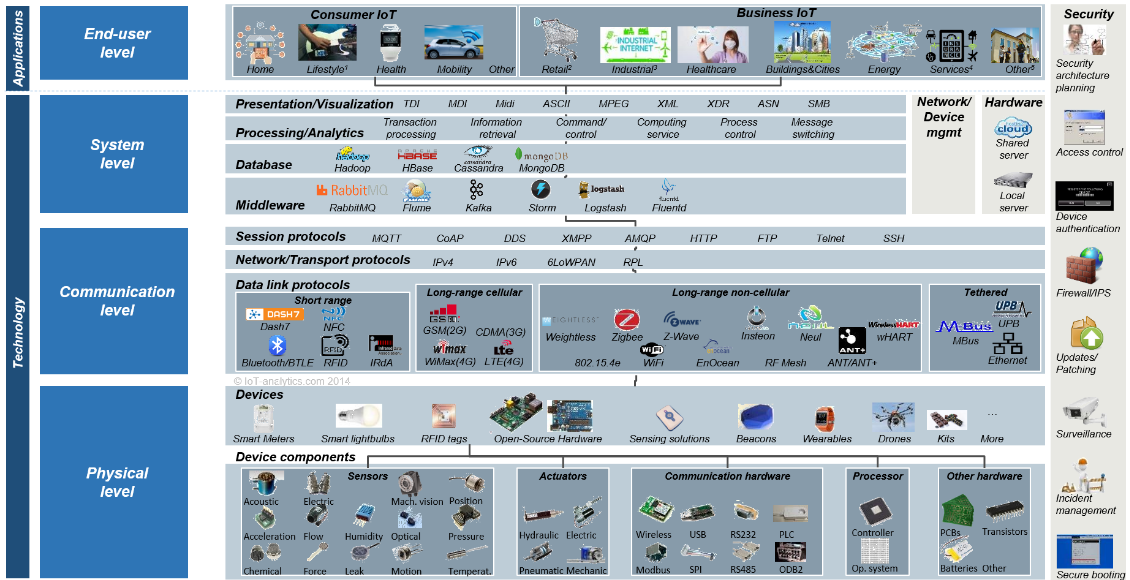
\includegraphics[width=0.99\textwidth]{31_iot.png}
\caption{IoT súhrn techológií \cite{IOT20}}
\label{31_iot}
\end{figure} 
Na obrázku je možné vidieť súčasti, ktoré sme uviedli ako spoločné črty IoT definícií. Pri pohľade na tento obrázok si je dôležité uvedomiť, koľko rôznych typov softvérov, jazykov a architektúr tu prichádza do interakcie. Začínajúc zo spodu. Senzory a akčné členy podľa zložitosti majú buď len nahratý jednoúčelový firmware, ktorý umožňuje len meranie prípadne vykonávanie akčných zásahov a posielanie dát. Alebo majú určitý druh operačného systému, ktorý umožňuje na tejto úrovni do merania a akčných zásahov robiť úpravy. Ak sa spomenie posielanie dát, tak opäť je tam softvér zodpovedný za odosielanie a prijímanie dát, pričom ako je možné vidieť na obrázku, tak je viacero úrovni abstrakcie odosielania údajov. Na systémovej úrovni sú to rôzne databázové systémy, systémy na spracovanie správ (message queue), analytické nástroje a vizualizačné rozhrania. Nakoniec až na najvyššej úrovni sú aplikácie, ktoré spojením rôznych pojmov z nižšej vrstvy dokopy majú pridanú hodnotu pre koncového používateľa. Na prvý pohľad by sa dalo povedať, že IoT sa nijako nelíši od existujúcich priemyselných inštalácií, preto je ďalej znázornené, v čom sa IoT líši od tradičnej architektúry priemyselných systémov na obrázkoch \ref{32_iotA} a \ref{32_iotB}.

\begin{figure}[!htbp]
\centering
\begin{subfigure}{0.5\linewidth}
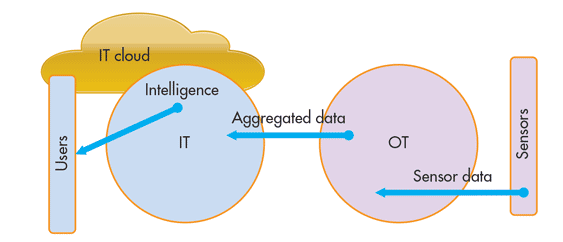
\includegraphics[width=0.9\textwidth]{32_iotA.png}
\caption{Tradičná architektúra \cite{IOT21}}
\label{32_iotA}
\end{subfigure}%
\begin{subfigure}{0.5\linewidth}
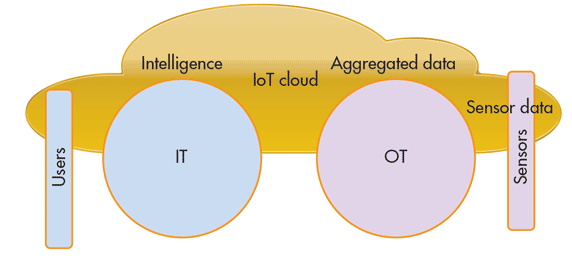
\includegraphics[width=0.9\textwidth]{32_iotB.png}
\caption{IoT architektúra \cite{IOT21}}
\label{32_iotB}
\end{subfigure}
\caption{Porovnanie tradičnej a IoT architektúry.}
\end{figure}
Tradičná priemyselná architektúra na posunutie dát do platformy informačných technológií (Information Technology - IT), ktorá vie robiť analýzu dát, poskytovať ich používateľovi aj vystavovať do cloud prostredia, používa vstavaný softvér na platforme obslužných technológií (Operational Technology - OT). IoT architektúra práve posúva väčšiu časť inteligencie systému z IT strany do OT strany. Toto umožňujú mikroprocesory a vstavané platformy s jednoduchým prístupom do cloud prostredia a rovnako s jednoduchým prístupom ku autorizovaným zariadeniam a používateľom. \cite{IOT21}. Táto definícia potvrdzuje to, čo sme už vyslovili, že ide o užšie prepojenie IT a OT. \\
\indent Základné ciele IoT architektúr je teda zosnímané dáta čo najskôr, najbezpečnejšie a najspoľahlivejšie poslať ďalej na miesto, kde môžu prejsť analýzou, či už je to cloud alebo dosť často to býva aj samotný agregátor, ktorý má dostatočný výkon na určitý druh analýz a na základe analýzy ovplyvniť akčné členy, aby sa optimalizoval proces, náklady, zdroje atď. Aktuálny trend vo svete je, že  veľké technologické firmy sa snažia spraviť univerzálnu IoT platformu a podchytiť si tak čo najviac zákazníkov. Veľké firmy typu Microsoft, Amazon, HP už pripravili svoje platformy, ktoré sa líšia v použitých technológiách, ale princíp ostáva rovnaký. Na demonštráciu sa uvádza porovnanie dvoch hotových platforiem Azure IOT HUB od Microsoft a AWS IOT od Amazonu v tabuľke \ref{table:1} a na obrázku \ref{33_aa}.
\begin{table}[h!]
\centering
 \caption{Porovnanie dvoch IOT platforiem \cite{IOT22} }
 \begin{tabular}{ |p{4cm}|p{5.5cm}p{5.5cm}| } 
 \hline
 Produkty & MS AZURE IOT HUB & AMAZON AWS IOT \\ 
 \hline\hline
 Protokoly & HTTP, AMQP, MQTT, vlastné protokoly & HTTP, MQTT  \\ 
 \hline
 Komunikačné vzory & Diaľkové meranie, príkazy & Diaľkové meranie, príkazy \\
 \hline
 Certifikované platformy &  Intel, Raspberry Pi 2, Freescale, Texas Instruments, MinnowBoard, BeagleBoard, Seeed, resin.io & 
Broadcom, Marvell, Renesas, Texas Instruments, Microchip, Intel, Mediatek, Qualcomm, Seeed, BeagleBoard \\
 \hline
 SDK/jazyky & 	.Net, Java, C, NodeJS & C, NodeJS \\
 \hline
\end{tabular}
\label{table:1}
\end{table}

\begin{figure}[!htbp]
\centering
\begin{subfigure}[b]{0.8\textwidth}
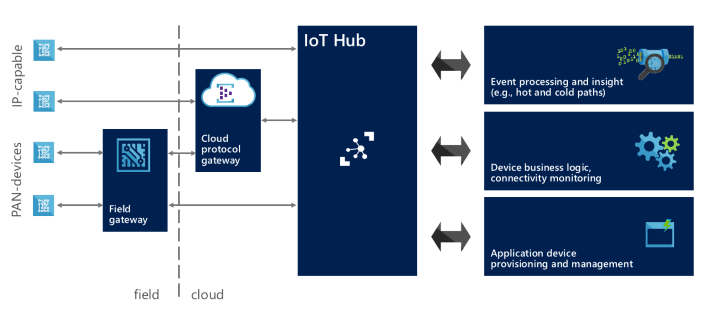
\includegraphics[width=1\linewidth]{33_azure.png}
\caption{Azure IOT HUB \cite{IOT22}}
\label{33_azure}
\end{subfigure}
\begin{subfigure}[b]{0.8\textwidth}
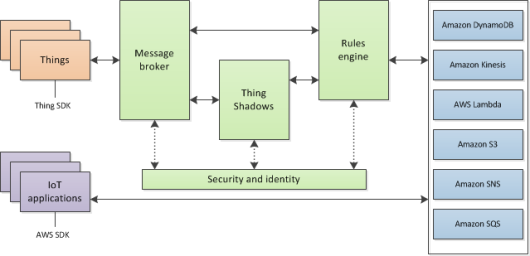
\includegraphics[width=1\linewidth]{33_aws.png}
\caption{AWS IOT \cite{IOT22}}
\label{33_aws}
\end{subfigure}
\caption{Porovnanie IoT platforiem.}
\label{33_aa}
\end{figure}
\indent Na portály Devexperience a stránke \cite{IOT22}, kde bolo porovnanie vykonané, definujú tieto súčasti IoT architektúry: \\
\indent Kompletné IoT riešenie pozostáva z viacero častí. Ako prvé je potrebné prijať všetky udalosti a dáta poslané zo zariadení a to je veľký problém, lebo v dobe internetu vecí je potrebné myslieť na škalovateľnosť v stovkách, tisíckach, miliónoch a ...  miliardách zariadení. Preto je potrebné mať \textbf{prijímací} (ingestion) systém, ktorý je schopný spracovať dáta veľmi rýchlo bez spomalenia celého procesu. Takto sa nazýva komunikačný vzor\textbf{ diaľkové meranie}. \\
\indent Po získaní dát, prijímací systém ich musí poskytnúť biznis pravidlovému systému. V spomenutých riešeniach môže byť použitá tzv. horúca cesta na analýzu dát ako tok dát v reálnom čase a tzv. studená cesta pre ukladanie dát pre budúce analýzy. Je možné to považovať za Big Data problém. Obidve cesty môžu vystaviť informácie konečnému používateľovi, ktorý môže sledovať, čo sa zo zariadeniami v reálnom svete deje. Rovnaká informácia je  užitočná pre systém strojového učenia, ktorý môže pri prediktívnej analýze napomôcť pochopiť ako sa dáta môžu vyvíjať v budúcnosti na základe aktuálnych hodnôt. \\
\indent Rovnako sa nesmie zabudnúť na opačnú cestu z cloud systému do zariadení. Vo väčšine prípadov na interakciu s nimi je potrebný vzor \textbf{príkazy} a \textbf{notifikácie}. Pomocou príkazov je možné komunikovať so zariadeniami, takže môžu vykonávať nejaké úkony. Pomocou notifikácií je možné poskytnúť zariadeniam informácie, ktoré potrebujú počas behu. Na zabezpečenie príkazov a notifikácií na komunikáciu s koncovými zariadeniami sa často používajú tzv. brány na komunikáciu zo zariadenia do cloudu a naopak často označovaný ako Cloud gateway. \\
\indent Všetky zariadenia by boli schopné pristupovať na Cloud gateway, keby boli pripojené pomocou ethernetových sietí s podporou TCP/IP protokolu. Pre zariadenia s obmedzením na prostriedky s využitím PAN (Personal Area Network) protokolov (napríklad Bluetooth, Zigbee, Z-Wave, rovnako je možné uvažovať na AllJoyn frameworkom) je potrebné uvažovať nad tzv. field gateway, ktorý vystupuje ako lokálna brána na prístup do cloud priestoru. Táto brána má úlohu prekladača protokolov a môže zabezpečovať lokálne ukladanie, filtrovanie a spracovanie úkonov, keď prídu dáta, ešte pred tým ako sa pošlú do cloud. Samozrejme to môže byť vstupný bod pre lokálny systém na prijímanie príkazov a notifikácii poslaných z cloud a smerovaných na zariadenia. \cite{IOT22}
Cieľom porovnania nie je zaoberať sa detailami implementácie jednotlivých riešení, ale poukázať na principiálnu podobnosť architektúr. Obrázok \ref{34_iot_fin} zovšeobecňuje a znázorňuje všetky súčasti a možnosti zapojenia hlavných súčastí IoT riešení, ktoré sú uvedené v predošlej citácií a rovnako sa uvádzajú vo väčšine literatúr. Finálne zovšeobecnenie jednotlivých komponentov IoT architektúry je nasledovné. 
\begin{itemize}
\item Snímač akčný člen, z ktorého komunikačná vrstva robí IoT zariadenie alebo naopak zariadenie s komunikačnou vrstvou a snímačom alebo akčným členom je IoT zariadenie. IoT zariadenie môže mať určitú výpočtovú kapacitu na jednoduchú automatizáciu procesu. Tiež môže mať výpočtovú kapacitu na obsluhu viacerých snímačov akčných členov a dočasné ukladanie dát. 
\item Ďalší prvok je IoT brána (Gateway, agregátor, field gateway), ktorá spravuje celú sieť IoT zariadení, komunikáciu s nimi, ich správu, pokročilú automatizáciu procesov a dátovú analýzu. Zvyčajne je rozhraním do cloud služieb, ak samotné IoT zariadenie nevie komunikovať priamo so službami v cloude. 
\item Posledným prvkom je IoT Backend (cloud služby), ktoré sú považované za neobmedzené kapacity priestoru, výkonu, kde môžu prebiehať zložité analýzy dát a zložitá automatizácia procesov.
\end{itemize}
\begin{figure}[!htbp]
\centering
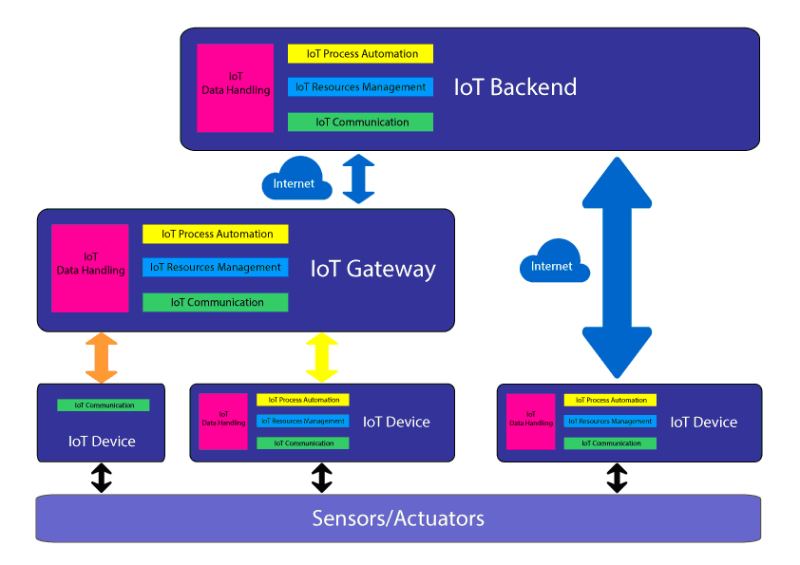
\includegraphics[width=0.99\textwidth]{34_iot_fin.png}
\caption{IoT súčasti - všeobecne\cite{IOT23}}
\label{34_iot_fin}
\end{figure} 

V tomto bode máme zadefinované všetky pojmy a princípy, ktoré sú potrebné pri návrhu reálnej IoT aplikácie s modernými metódami riadenia a teda spojenia oblasti automatizácie a softvérovéj architektúry. 


\subsubsection{Oblasti využitia}
Po zadefinovaní hlavných súčasti architektúry IoT riešení, prácav krátkosti popisuje oblasti využitia IoT. Ako podklad pre vymenovanie je dokument \cite{IOT24}.
\begin{itemize}
\item IT a siete - verejné, podnikové (PC, router, switch, pobočkové ústredne, ...).
\item Digitálna a verejná bezpečnosť - verejné osvetlenie, kamerové systémy...
\item Obchod - digitálne popisky, registračné pokladnice, ... 
\item Doprava - lode, lietadla, autá, mýta, ...
\item Priemysel - distribučné siete, automatizácia zdrojov, ...
\item Zdravotná starostlivosť - telemedicína a sledovanie pacientov, ...
\item Energetika - optimalizácia dopytu a ponuky, podpora efektivity alternatívnych zdrojov, ...
\item Komerčné budovy - správa budov, úspora na prevádzkovanie, ...
\item Domácnosť a spotrebiteľ - pohodlie a zábava, spotrebiče, ...
\end{itemize}
Pre návrh a implementáciu bol zvolený  IoT systém inteligentnej domácnosti, ktorého špecifiká sú v práci priebežne menované. Týmto končí časť definícii a nasleduje popis technických krokov návrhu a vývoja IoT systému a aplikovania MPC do tohto systému.
\section{Návrh a implementácia IoT systému s modernými metódami riadenia}
Táto časť popisuje postup návrhu a implementácie aplikácie moderných metód riadenia do IoT prostredia. Pod modernými metódami riadenia sa rozumie zavedenie nového pojmu controller as a service (CaaS) - regulátor ako služba a pod IoT prostredím sa tu rozumie inteligentná domácnosť. Myšlienka CaaS je výsledkom sledovania IoT trendu a návrh je inšpirovaný IoT architektúrami v dvoch bodoch. Prvý bod je využitie potenciálu výpočtového výkonu serverov. Vstavané zariadenia sa ukázali ako nedostatočné pre vykonávanie online MPC výpočtu. Druhý bod je užšia spolupráca serveru a akčného člena.  Návrh konkrétnej realizácie je založený na SOA architektúre s REST princípmi. Viac je popísane v časti \ref{caas}. 
Teraz nasleduje popis IoT prostredia s odôvodnením voľby kľúčových elementov s ohľadom na finálnu architektúru.
\subsection{Popis a voľba experimentálneho IoT prostredia} \label{iotenv}
Cieľová architektúra vychádza z obrázkov \ref{31_iot} a \ref{34_iot_fin}. IoT prostredie preto pozostáva z týchto prvkov:
\begin{itemize}
\item Fyzická vrstva - snímače.
  \begin{itemize}
    \item Svetelný senzor.
      \begin{itemize}
        \item Aeotec MultiSensor 4-in-1.
        \item Slim Multi-Sensor PSM01. 
        \item Fotorezistor napojený na AD/DA prevodník s PCF8591 čipom
       \end{itemize}
    \item Teplotný senzor.
      \begin{itemize}
        \item Aeotec MultiSensor 4-in-1.
        \item Slim Multi-Sensor PSM01.        
        \item Oregon Scientific WMR 88. 
       \end{itemize}    
    \item Senzor vlhkosti.
      \begin{itemize}
        \item Aeotec MultiSensor 4-in-1.
        \item Slim Multi-Sensor PSM01.        
        \item Oregon Scientific WMR 88. 
       \end{itemize}     
    \item Pohybový senzor.
      \begin{itemize}
        \item Aeotec MultiSensor 4-in-1.
        \item Vision ZP3102 EU PIR Motion Sensor.        
       \end{itemize}     
    \item Okenný/dverový senzor na magnetickom princípe.
      \begin{itemize}
        \item Slim Multi-Sensor PSM01.
        \item FIBARO FGK 101-107.        
       \end{itemize}            
    \item Záplavový senzor.    
      \begin{itemize}
        \item FIBARO FGFS 101.        
       \end{itemize}                
    \item Senzor intenzity a smeru vetra.    
      \begin{itemize}      
        \item Oregon Scientific WMR 88. 
       \end{itemize}         
    \item Senzor barometrického tlaku.        
      \begin{itemize}      
        \item Oregon Scientific WMR 88. 
       \end{itemize}             
    \item Tlačítko.     
      \begin{itemize}      
        \item Z-Wave.Me Wall Controller 06443. 
        \item Z-Wave.Me Wall Controller WallC.
       \end{itemize}             
  \end{itemize}
\item Fyzická vrstva - akčné členy.
  \begin{itemize}
    \item Termostatická hlavica.
      \begin{itemize}      
        \item Danfoss living connect Z. 
       \end{itemize}     
    \item Spínacie relé.
      \begin{itemize}      
        \item PAN04 Dual realy.         
       \end{itemize}     
    \item Univerzálny stmievač.    
      \begin{itemize}      
        \item FIBARO FGD 211.         
        \item Aeotec Micro Smart Dimmer. 
        \item Z-Wave.Me Wall Flush-Mountables.                 
       \end{itemize}         
    \item Spínacia zásuvka.     
      \begin{itemize}      
        \item FIBARO FGWPE/F 101.         
       \end{itemize}     
  \end{itemize}  
\item Fyzická vrstva - komunikačný hardware.
  \begin{itemize}
    \item USB
    \item $I^2C$
  \end{itemize}    
\item Fyzická vrstva - Zariadenia.
  \begin{itemize}
    \item Raspberry Pi model A+
    \item Raspberry Pi 2 model B    
    \item Vera Control VeraLite
  \end{itemize}  
\item Komunikačná vrstva smer IoT zariadenie gateway.
  \begin{itemize}
    \item Z-Wave
    \item RSS (HTTP)
    \item REST (HTTP)    
  \end{itemize}    
\item Komunikačná vrstva smer gateway IoT Backend.
  \begin{itemize}
    \item REST (HTTP)
  \end{itemize} 
\item Systémová vrstva.
  \begin{itemize}
    \item MongoDB databáza 
    \item Jersey REST interface
    \item Matlab/Octave  nástroje na výpočty     
    \item JSON komunikačné rozhranie
    \item InfluxDB
    \item Grafana
  \end{itemize}           
\item Používateľská vrstva.
  \begin{itemize}
    \item Správa inteligentnej domácnosti
    \item Vizualizácia nameraných údajov 
    \item Aplikácie s pridanou hodnotu 
  \end{itemize}         
\end{itemize}
\begin{figure}[!htbp]
\centering
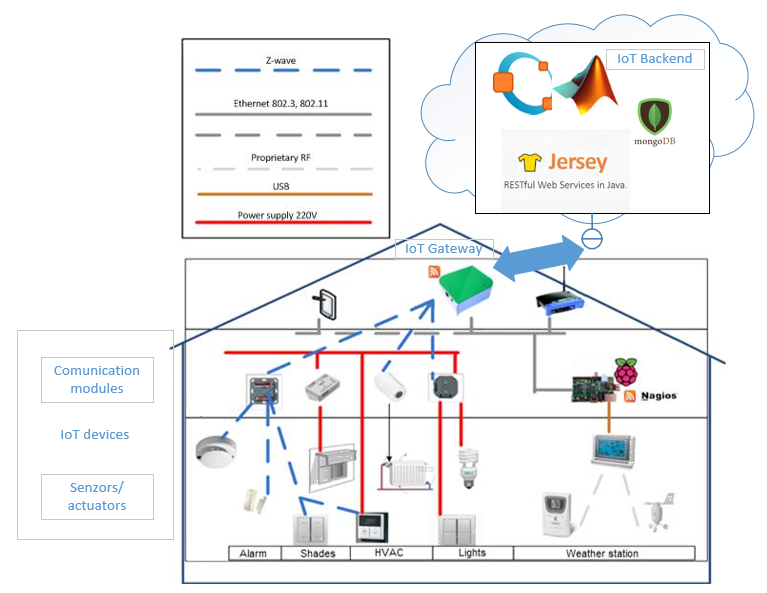
\includegraphics[width=0.99\textwidth]{35_schema.png}
\caption{Experimentálne prostredie}
\label{35_schema}
\end{figure} 
Fyzická vrstva sa skladá z vymenovaných senzorov a akčných členov, z ktorých väčšina je pripojená do systému pomocou protokolu Z-Wave. Protokol Z-Wave je bezdrôtový protokol stredného dosahu v Európe fungujúci na frekvenciách 868.42MHz,   ktorý potrebuje na svoje fungovanie jeden hlavný uzol, ktorý spravuje sieť a identifikáciu zariadení. Architektonické rozhodnutie, pri návrhu IoT prostredia, pre voľbu Z-Wave protokolu bol fakt, že Z-Wave je bezdrôtový a zariadenia je možné implementovať do existujúcej elektrickej inštalácie. Požiadavka implementácie do existujúcej elektrickej inštalácie vychádza z ekonomického aspektu a z potreby overenia možnosti vytvárania IoT prostredia v byte, a teda s obmedzenejšími možnosťami na zásahy do ovládania kúrenia, merania spotrieb a podobne oproti klasickým domom. Spomínaný hlavný uzol v navrhovanom prostredí je zariadenie VeraLite. Existuje viacero alternatív ku tomuto zariadeniu, ktoré majú svoje výhody a nevýhody. Architektonické argumenty pre voľbu tohto zariadenia boli stabilita, možnosť custom vývoja a nižšia cena oproti iným. Zariadenie od spoločnosti Fibaro \cite{IOT25} je vysoko stabilné, ale neumožňuje veci programovať a aj cena je rádovo vyššia. Zariadenie Vera3 \cite{IOT27} je vyššia verzia zariadenia VeraLite, ktoré je ešte stabilnejšie, ale aj pomerne drahšie. Ďalšie uvažované zariadenie bolo RaZberry \cite{IOT26}, ktoré sa predáva ako pripojiteľný modul so Z-wave komunikačným rozhraním ku zariadeniu Raspberry Pi, ktoré by zohrávalo úlohu hlavného uzlu. Cena aj možnosť programovania tu boli výborne avšak stabilita nebola dostatočná. Preto hlavný uzol siete Z-Wave zohráva zariadenie VeraLite. Pomocou tohto zariadenia sú jednotlivé fyzické zariadenia pridávané do siete. Dôležitou vlastnosťou je, že okrem fyzických zariadení vie toto zariadenie pridávať aj \textbf{zariadenia softvérové}, čo súvisí s možnosťou programovateľnosti. Softvérovým zariadeniam sa bude venovať neskôr. Spôsob pridávania fyzických zariadení do siete Z-Wave funguje na základe špeciálneho módu (inclusion mode), ktorý je potrebné nastaviť na hlavnom uzle. Hlavný uzol vtedy počúva a očakáva sekvenciu príkazov, pomocou ktorých identifikuje nové zariadenie a zaregistruje ho do siete - proces nazývaný inclusion. Pridávané zariadenie rovnako musí byť nastavené do inclusion módu. Spôsob zapnutia inclusion módu je plne na výrobcovi zariadenia väčšinou to je určitá sekvencia stlačenia tlačítka. Pri senzoroch sú to zvyčajne špeciálne tlačítka pre účely nastavovania sieťových parametrov. Pri ostatných zariadeniach sa využívajú používateľské tlačítka. Po zaregistrovaní zariadenia do siete hlavný uzol vie zariadenie ovládať a pýtať sa na aktuálny stav. Zariadenie VeraLite v našom IoT systéme, ako je možné vidieť na obrázku \ref{35_schema} zohráva úlohu brány. \\
\indent Ďalšie zariadenie pripojené v IoT systéme je meteostanica a to prostredníctvom USB káblu na zariadenie Raspberry Pi model A. Meteostanica pozostáva z vnútornej zobrazovacej jednotky, na ktorej je meraná vnútorná teplota a vlhkosť, vonkajšieho snímača teploty, vlhkosti a atmosferického tlaku,  merača úhrnu zrážok a anemometra na meranie intenzity a smeru vetra. Komunikácia medzi snímačmi a vnútornou jednotkou je prostredníctvom rádiového signálu na frekvencii 433 MHz. Na Raspberry Pi beží operačný systém Raspbian, špeciálna verzia distribúcie Debian. V operačnom systéme beží aplikácia \textit{wview}, ktorá komunikuje s USB portom a ukladá údaje do \textit{sqlite} databázy, robí tzv. dočasné úložisko. Síce dlhodobejšie ako je pamäť na zobrazovacej jednotky, ktorá ukladá posledných 24 hodín, ale nie je to úložisko, na ktoré sa možno spoľahnúť. \\ 
\indent Ďalší spôsob pripojenia do IoT systému tvorí fotorezistor s PCF8591 čipom cez GPIO rozhranie pripojené do zariadenia Raspberry pi 2 Model B+. Dôvod voľby tejto kombinácie do IoT systému je možnosť prístupu na najnižšiu úroveň ovládania zariadenia. Pri ostatných Z-Wave zariadeniach je firmware daný a ak je obmedzená minimálna hodnota periódy vzorkovania na hodnotu, ktorá nie je dostatočná pre identifikáciu systému, je potrebné mať možnosť zariadenia, v ktorom dané parametre možno zmeniť. Spôsob vystavania hodnoty fotorezistora do IoT prostredia je vďaka takémuto súboru aplikácií:
\begin{itemize}
\item základ tvorí operačný systém typu Linux, špeciálna edícia Debian distribúcie pre Raspberry Pi.
\item Nadstavbu tvorí Node.js framework, ktorý umožňuje vytvárať udalosťami riadené  systémy.
\item V Node.js frameworku je v jazyku Javascript vytvorená aplikácia, ktorá 
  \begin{itemize}
  \item umožňuje komunikovať s GPIO rozhraním a tak načítať hodnotu zo senzora.
  \item Prekladá údaj o odpore zo svetlocitlivého fotorezistora na údaj zodpovedajúcemu intenzite osvetlenia a
  \item poskytuje nameranú hodnotu prostredníctvom REST rozhrania.
  \end{itemize}
\end{itemize} 
Fyzikálna veličina odporu je takto skonvertovaná do digitálnej podoby a takto prístupná takému zariadeniu, ktoré vie vytvoriť HTTP požiadavku a prečítať jej odpoveď.
 
\subsubsection{Detaily IoT brány}
Táto kapitola sa detailne venuje
\begin{itemize}
  \item popisu VereLite zariadenia.
  \item Spôsobu komunikácie zariadení Raspberry Pi s VeraLite (IoT bránou).
  \item Spôsobu programovania zariadenia VeraLite a vytvárania softvérových zariadení v ňom, ktoré sú demonštráciou úzkeho prepojenia IT s OT. Ďalej sa prostredníctvom nich demonštrujú výhody SOA architektúry a REST princípov.   
\end{itemize} 
Výrobcovia zariadení rodiny Vera si ako základný prvok postavili Linux systém. Na VeraLite beži distribúcia OpenWrt. Framework na ovládanie IoT zariadení je postavený na protokole UPnP - priemyselný štandard na ovládanie zariadení, a skriptovacom jazyku Lua. Framework sa volá \textit{Luup} \cite{IOT28}.\\ 
\indent Vďaka UPnP je možné definovať zariadenia, jeho služby, stavové premenné služby, operácie služby a parametre na vstupe a výstupe operácie. Ako príklad definície zariadenia uvádzame spínané svetlo a stmievané svetlo.\\
\indent ID definície spínaného zariadenia je \textit{urn:schemas-upnp-org:device:BinaryLight:1}. Spínané svetlo má len jednu službu a jej ID je \textit{urn:upnp-org:serviceId:SwitchPower1}. Jediná premenná tejto služy je \textit{Status}, ktorá môže nadobúdať hodnoty 0, ak je svetlo vypnuté a 1, ak je svetlo zapnuté. Jedina operácia tejto služby \textit{SetTarget}, ktorá má na vstupe parameter s názvom \textit{newTargetValue}. Ukážka zapnutia svetla je v algoritme \ref{alg01}. 
\begin{algorithm}
\lstset{
    language=C,
    basicstyle=\small\sffamily,
    frame=none,
    numbers=left,
    xleftmargin=5.0ex,
    numberstyle=\tiny,
    stepnumber=1,
    showstringspaces=false,
    keywordstyle=\color{blue}\bfseries
    }
\lstset{emph={%  Adjust any special keywords
    printf%
    },emphstyle={\color[rgb]{1,0,0}\bfseries}%
}%
\begin{lstlisting}
luup.call_action("urn:upnp-org:serviceId:SwitchPower1",
                 "SetTarget", {newTargetValue = "1"}, 37)
\end{lstlisting}
 \caption{Zapnutie svetla}
 \label{alg01}
\end{algorithm}

Funkcia call\_action frameworku \textit{Luup} robí zmenu nastavenia UPnP premennej prostredníctvom funkcie, ktorá bola pri špecifikácii služby zariadenia na to určená. Parametre potrebné na túto zmenu sú meno služby, meno funkcie, meno vstupnej premennej, jej hodnota a nakoniec ID inštancie zariadenia v systéme. ID inštancie je vytvárané tak pre fyzické zariadenia, ako aj pre softvérové zariadenia.\\
\indent Stmievané svetlo má ID definície \textit{urn:schemas-upnp-org:device:DimmableLight:1}. Má dve služby. Má aj službu \textit{urn:upnp-org:serviceId:SwitchPower1}, ktorú má spínané svetlo, keďže aj stmievané svetlo je možne vypnúť ako spínané. Navyše má službu \textit{urn:upnp-org:serviceId:Dimming1}, ktorá pomocou premennej operácie \textit{SetLoadLevelTarget} a vstupnej premennej \textit{newLoadlevelTarget} nastavuje stavovú premennú \textit{LoadLevelStatus}. Čím sa nastavuje percento intenzity zotmenia. Kód na zistenie stavu stmievaného svetla vo frameworku \textit{Luup} je zobrazený v algoritme \ref{alg02}.
\begin{algorithm}
\lstset{
    language=C,
    basicstyle=\small\sffamily,
    frame=none,
    numbers=left,
    xleftmargin=5.0ex,
    numberstyle=\tiny,
    stepnumber=1,
    showstringspaces=false,
    keywordstyle=\color{blue}\bfseries
    }
\lstset{emph={%  Adjust any special keywords
    printf%
    },emphstyle={\color[rgb]{1,0,0}\bfseries}%
}%
\begin{lstlisting}
lightLevel = luup.variable_get("urn:upnp-org:serviceId:Dimming1", 
                               "LoadLevelStatus", 37)

\end{lstlisting}
 \caption{Načítanie stavu stmievaného svetla}
 \label{alg02}
\end{algorithm}
Na základe tejto generickosti UPnP protokolu sa v práci definovalo šesť nových typov zariadení, štyri pomocné a dve zariadenia nevyhnutné pri implementácii CaaS.
Začneme s popisom jednoduchších, pomocných a následne prejdeme k tým dôležitým.
\begin{itemize}
  \item Zariadenie typu barometer s ID  \textit{urn:schemas-micasaverde-com:device:Barometer:1} a službou \textit{urn:upnp-org:serviceId:Barometer1}, ktorá bola vytvorená na základe zariadenia pre snímanie teploty so zmenou mena stavovej premennej na \textit{CurrentAirPressure}
  \item Zariadenie typu veterný snímač s ID  \textit{urn:schemas-micasaverde-com:device:WindSensor:1} a službou \textit{urn:upnp-org:serviceId:WindSensor1}. Toto zariadenie pozná stavové premenné \textit{WindSpeed} a \textit{WindDirection}. Obe vytvorené zariadenia, nemajú operáciu na zadávanie hodnoty, keďže sú to senzory. Používateľ pri nich nemá a ani nemá mať možnosť zadávať hodnotu, má iba možnosť hodnoty zo senzora čítať.
  \item  Na komunikáciu VeraLite s Raspberry PI model A a čítanie hodnôt z meteostanice sa vo VeraLite vytvorilo všeobecné softvérové zariadenie typu RSS Reader s ID zariadenia \textit{urn:demo-micasaverde-com:device:RssReader:1}.
  \item Na komunikáciu VeraLite s Raspberry PI model B a čítanie hodnôt z fotorezistora sme vytvorili všeobecné zariadenie Rest Handler, všeobecne na čítanie akejkoľvek rest služby s ID \textit{urn:demo-micasaverde-com:device:RestHandler:1}.
\end{itemize} 
To boli pomocné softvérové zariadenia, ktoré rozširujú možnosti komunikácie a dátové body zariadenia VeraLite a pripravujú IoT prostredie na aplikovanie prediktívnych metód riadenia do systému. Nasleduje krátky opis RSS Reader a REST Handler zariadení a následne bude kapitola venovaná aplikácii MPC v IoT systéme.

\indent RSS Reader predstavuje zariadenie, ktoré pravidelne odoberá novinky z webových stránok vo formáte XML. Vďaka tomu, okrem toho, že je možné sa napojiť na odber akýchkoľvek noviniek z bežných webových stránok, je možné sa napojiť aj na aplikáciu \textit{wview}, ktorá v popisovanom systéme beží na Raspberry Pi model A. Do tela noviniek generovaných aplikáciou \textit{wview} sa nakonfigurovalo, aby sa tam vkladalo XML v špecifickom tvare, v ktorom sú uložené dáta zo senzorov meteostanice. 
Ukážka časti konfiguračného súboru je v algoritme \ref{alg03}.
\begin{algorithm}
\lstset{
    language=XML,
    basicstyle=\small\sffamily,
    frame=none,
    numbers=left,
    xleftmargin=5.0ex,
    numberstyle=\tiny,
    stepnumber=1,
    showstringspaces=false,
    keywordstyle=\color{blue}\bfseries
    }
\lstset{emph={%  Adjust any special keywords
    printf%
    },emphstyle={\color[rgb]{1,0,0}\bfseries}%
}%
\begin{lstlisting}
...
<item>
  <title><!--stationCity-->,<!--stationState--> </title>
      <link>Insert_Your_WX_HomePage_URL_Here</link>
      <description>Current Weather Conditions</description>
      <pubDate><!--stationTime-->, <!--stationDate--></pubDate>
      <dc:date><!--stationDate--> - <!--stationTime--></dc:date>
	  <!-- vera specific content -->
	  <temperature>
	    <sensor id="0" attr="inside" descr="" >
		  <value><![CDATA[<!--insideTemp-->]]></value>
		  <unit><![CDATA[<!--tempUnit-->]]></unit>
		</sensor>
	    <sensor id="1" attr="outside" descr="" >
		  <value><![CDATA[<!--outsideTemp-->]]></value>
		  <unit><![CDATA[<!--tempUnit-->]]></unit>
		</sensor>
	  </temperature>
  </title>
</item>
...
\end{lstlisting}
 \caption{Časť konfiguračného súboru na vytvorenie XML k odberu noviniek}
 \label{alg03}
\end{algorithm}

Takto sa zabezpečí, že v odbere noviniek zo ,,serveru`` s meteostanicou je pravidelne podávaná informácia o senzorických dátach, v prípade práce to je konkrétne vnútorná a vonkajšia teplota, vnútorná a vonkajšia vlhkosť, intenzita a smer vetra a barometrický tlak. V grafickom rozhraní na nastavenie aplikácie \textit{wview} sa volí ako často sa majú dáta publikovať. Týmto je vybavená  strana poskytovateľa údajov. Pokračuje sa v opise RSS Reader softvérového zariadenia naprogramovaného v \textit{Luup} frameworku. Základné súčasti programu naprogramované v jazyku Lua, ktoré možno jednoducho pridať do \textit{Luup} frameworku, sú  modul \textit{socket.http}, ktorý slúži na poslanie HTTP GET požiadavky na ,,server`` s meteostanicou alebo url na odoberanie noviniek. Ďalej to je XML parser, ktorý bol stiahnutý ako open-source zdrojový kód a použitý na čítanie jednotlivých položiek v novinkách a na čítanie definovaného tvaru XML, ktoré chodí z meteostanice. V programe je definovaný prepínač, ktorý umožní, aby na základe prečítaných dát z meteostanice sa vytvorili samostatné ,,podzariadenia`` vytvárane RSS Reader zariadením, ktoré sú typu teplotného senzoru, senzoru vlhkosti a všetky ostatné, ktoré boli vyššie vymenované. V grafickom rozhraní pre používateľa to vyzerá tak, ako je znázornené na obrázku \ref{36_veragui}. 
\begin{figure}[!htbp]
\centering
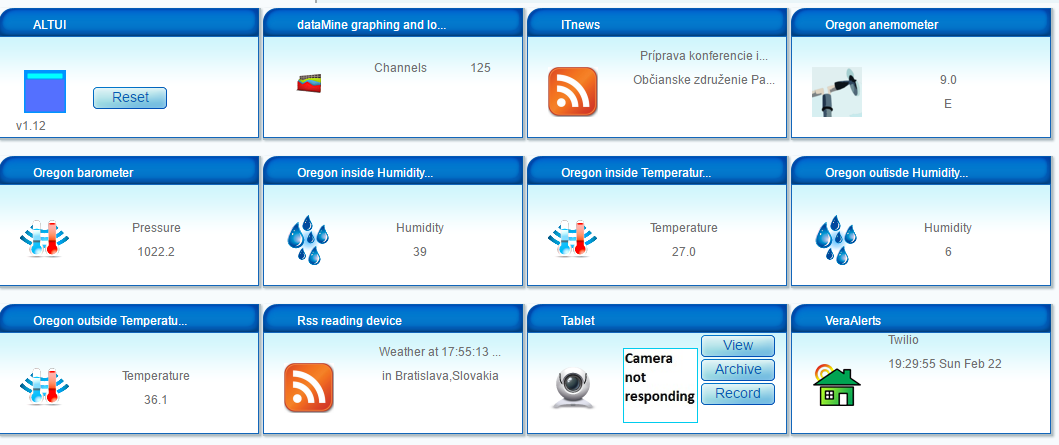
\includegraphics[width=0.99\textwidth]{36_veragui.png}
\caption{Vera GUI - vytvorené softvérové zariadenie}
\label{36_veragui}
\end{figure} 
Na obrázku je zariadenie s popisom \textit{Rss reading device} hlavné zariadenie, ktoré vytvorilo všetky ,,podzariadenia`` s prefixom Oregon. Výhoda tohto prístupu je, že v automatizačných skriptoch sa možno rovno dopytovať na údaj z meteostanice a vyzerá to akoby teplota bola snímaná Z-Wave zariadením, keďže VeraLite je primárne hlavný uzol Z-Wave zbernice. Súčasti, ktoré je potrebné pri tvorbe softvérového zariadenia vytvoriť:
\begin{itemize}
  \item Definíciu zariadenia pre RSS Reader, čo je \textit{D\_RssRead.xml}. XML súbor kde je definované ID definície a služby, z ktorých pozostáva. V tomto prípade služba \textit{urn:demo-micasaverde-com:serviceId:RssRead1}.
  \item Ďalej je potrebné vytvoriť definíciu služby v tomto prípade ID služby z predošlého bodu je definované v súbore \textit{S\_RssRead.xml}. Tu sa nachádzajú stavové premenné a operácie. Najdôležitejšie stavové premenné sú URL a prihlasovacie údaje v prípade zabezpečenej URL. Riešený je len prípad zabezpečenia Basic authentication technológiou. Potom je tam niekoľko pomocných premenných a následne tieto operácie:
  \begin{itemize}
    \item SetURL - nastavenie URL adresy servera.
    \item SetUser - nastavenie prihlasovacieho mena.
    \item SetPass - nastavovanie hesla.
    \item SetSelected - nastavovanie zvolenej položky v prípade, ak server vráti viacero položiek v odbere noviniek. Nemôže sa stať v prípade odberu noviniek z meteostanice, lebo XML je definované tak, že tam je len jedna položka.
    \item SetRefPeriod - nastavenie času ako často sa má RSS Reader spýtať servera na aktuálne hodnoty. Tu si treba všimnúť, že je uplatnený princíp pravidelného pýtania, namiesto asynchronného prístupu, ktorý by bol lepší, ale náročnejší na zdroje aj na strane klienta ja na strane servera a navyše to \textit{Luup} framework nepodporuje.
    \item GetFeed - akcia na vyžiadanie si najnovších noviniek kliknutím. Bez zásahu používateľa je táto akcia pravidelne volaná podľa periódy nastavovanej v predošlej funkcii.
  \end{itemize}  
  \item Ak je zadefinované zariadenie, služba, operácie a stavové premenné, tak je potrebné ich implementovať v špecifickom súbore. Pre RSS Reader to je \textit{I\_RssRead.xml}. V tomto súbore je implementácia jednotlivých operácii. Keďže to je XML súbor, môže sa v tom komplikovane vyvíjať komplexná funkcionalita, preto je možné komplexnú logiku v Lua skripte programovať do špeciálneho súboru pre RSS Reader to je \textit{L\_RssRead.lua}. 
  \item Nakoniec Vera rozhranie s \textit{Luup} frameworkom umožňuje definovať vzhľad ako sa bude na GUI softvérové zariadenie zobrazovať. Toto je konfigurované v JSON súbore (\textit{D\_RssRead.json}). Je to pomerne obmedzený a ťažkopádny vývoj rozhrania, ale je to daň za konfiguračnú unifikovanosť. Vzhľad RSS Reader zariadenia je zobrazný na obrázku  \ref{36_veragui} a nastavenia RSS Reader zariadenia na obrázku \ref{38_rssoregon}.  
\end{itemize}
\begin{figure}[!htbp]
\centering
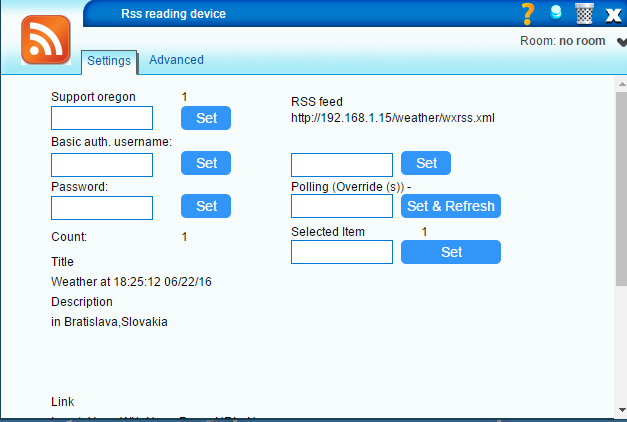
\includegraphics[width=0.7\textwidth]{38_rssoregon.png}
\caption{Nastavenia RSS Reader zariadenia}
\label{38_rssoregon}
\end{figure} 
Potom ako je všetko zadefinované, Vera poskytuje vývojárske rozhranie, kde sa spomínané súbory vložia a tým Vera pozná nové zariadenia, ktoré ma definované v XML súboroch, ktorých štruktúra je daná UPnP protokolom. Inštancia zariadenia však stále nie je vytvorená. Na to existuje ďalšie rozhranie, kde sa definuje ID definície zariadenia a jeho meno. Následne Vera vytvorí inštanciu zariadenia a priradí mu jednoznačné ID inštancie, podľa ktorého je možné sa dopytovať na stavové premenné alebo vykonávať operácie podľa algoritmov \ref{alg01} a \ref{alg02}.

\indent Rest Handler softvérové zariadenie funguje na veľmi podobnom princípe ako RSS Reader. Má len jednu službu s menom HandleRest, ktorej ID je  \textit{(urn:demo-micasaverde-com:serviceId:HandleRest1)} - spracuj REST službu, čo znamená, že program pravidelne oslovuje vystavený REST interface, ktorý poskytne dáta, v našom prípade informáciu z fotorezistora. Ohľadne implementácie, opäť je potrebné použiť modul na vytvorenie HTTP klienta a v tomto prípade je formát správ v JSON notácii, takže miesto XML parsera je tu použitá knižnica \cite{IOT30} na konverziu JSON objektov. Základne operácie definovane v službe sú nasledovné.
\begin{itemize}
\item setRestUrl - operácia na zadefinovanie URL, na ktorú sa ma HTTP klient dopytovať.
\item handleRest - operácia na samotné spustenie programu na pravidelné načítavanie hodnôt. Je potrebné definovať REST zdroj, HTTP metódu, ktorá sa ma použiť, perióda s akou ma byť REST zdroj volaný a objekt, z ktorého sa ma čítať výstupná hodnota.
\item (un)setBypass - operácie na zastavenie načítavania hodnôt.
\end{itemize}
Rozhranie na zadanie hodnôt a spustenie je zobrazené na obrázku \ref{44_gpio}.
\begin{figure}[!htbp]
\centering
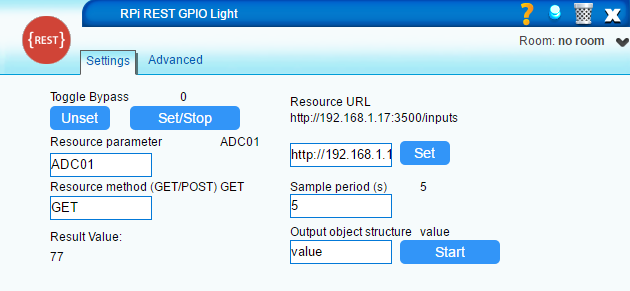
\includegraphics[width=0.85\textwidth]{44_gpio.png}
\caption{Rozhranie na zadávanie parametrov REST klienta.}
\label{44_gpio}
\end{figure} 
Výstup, ktorý REST rozhranie poskytne má tvar naznačený v algoritme \ref{alg06}.
\begin{algorithm}
\lstset{
    language=XML,
    basicstyle=\small\sffamily,
    frame=none,
    numbers=left,
    xleftmargin=5.0ex,
    numberstyle=\tiny,
    stepnumber=1,
    showstringspaces=false,
    keywordstyle=\color{blue}\bfseries
    }
\lstset{emph={%  Adjust any special keywords
    printf%
    },emphstyle={\color[rgb]{1,0,0}\bfseries}%
}%
\begin{lstlisting}
{
   "pin":0,"gpio":"ADC01","AIN":1,"value":75
}
\end{lstlisting}
 \caption{Príklad odpovede zo snímača vystaveného REST princípom.}
 \label{alg06}
\end{algorithm}  
Z odpovede je možné vidieť, že takto by bolo možné osloviť ktorýkoľvek pin GPIO rozhrania Raspberry PI a tak s pomocou jedného zariadenia poskytovať rozhranie ku celej množine senzorov a akčných členov. V našom prípade je pripojený len fotorezistor. 

\indent Toto bola ukážka ako programovať do špecifickej IoT brány (VeraLite), ktorá okrem obsluhy Z-Wave zariadení umožňuje ovládať aj zariadenia komunikujúce s TCP protokolom a jeho nadstavbami (HTTP, RSS, REST...). Tvorcovia Luup framewroku si zvolili mikrokernel (plugin) architektúru, kde hlavné jadro je implementované a kto čo potrebuje si môže v podobe pluginu naprogramovať a pridať do mikrokernel prostredia. Pre nás táto voľba je prínosná, pretože takýmto spôsobom je možné pripojiť akúkoľvek servisnú aplikáciu do systému a teda môžeme vidieť výhody správne zvolenej architektúry softvéru.\\
\indent Ďalej si tu môžeme uvedomiť otvorenosť UPnP protokolu a možnosti definovania vlastných zariadení pomocou neho. Čo v sumáre predstavuje štandardom podporenú mikrokernel architektúru, keďže UPnP je definované v ISO/IEC 29341 štandarde. Všetky doteraz menované aj neskôr spomenuté softvérové zariadenia, vytvorené v práci, sú dostupné pre využívanie používateľmi Vera zariadenia prostredníctvom github platformy. Nasleduje najdôležitejšia časť práce.


\subsection{CaaS - Regulátor ako služba} \label{caas}
Táto kapitola sa zameriava na vysvetlenie, motiváciu a opis implementácie myšlienky regulátor ako služba (Controller as a Service). Ako už bolo naznačené ide o vystavovanie služby regulovania procesu do cloud prostredia. Kedy na servery je uložený matematický model regulátora a na požiadavku vie server vrátiť akčný zásah pre daný regulátor v danom stave. Od klienta sa očakáva, že vie obsluhovať HTTP komunikáciu a základnú prácu s reťazcami, žiadne výpočty nevykonáva, len sa pravidelne spýta na akčný zásah. Pre regulátory s nízkymi nárokmi na výpočtovú kapacitu tento koncept nepridáva hodnotu výpočtového výkonu serveru, iba možnosť uloženia veľa inštancií, takže sa môže využiť iba pamäťová kapacita servera. Tento princíp dáva zmysel hlavne pre regulátory s veľkými požiadavkami na výpočtový výkon. Medzi takéto patrí práve online metóda MPC algoritmu, ktorý si vyžaduje, ako je v prvých kapitolách naznačené, prácu s veľkými maticami ich násobenie a  inverzia. Až niekoľko neúspešných pokusov v postupe práce priviedli k tomuto konceptu. Prvotné úvahy boli implementovať algoritmus popísaný v kapitole \ref{mpcalg} do jazyka, ktorý je blízky strojovému, aby bolo možné dať regulátor čo najbližšie procesu a teda ku zariadeniu, ktoré nemá veľký výpočtový výkon. Na toto boli použité konverzné metódy Matlab skriptov na spustiteľné súbory v jazyku C. Tieto pokusy neboli úspešné. Paralelne prebiehali aktivity implementácie MPC algoritmu na FPGA zariadenia, kde sa rovnako narážal na problem inverzie matíc a ďalších problémov, ktoré kvadratické programovanie prináša. Preto bol pre FPGA implementovaný explicitný - offline MPC regulátor. Tejto problematike sa venuje iná dizertačná práca. Predchádzajúce fakty z oblasti softvérovej architektúry a štúdium IoT architektúr priviedli na myšlienku CaaS a teda proces riadený pomocou regulátora, uloženého a výpočty vykonávajúceho na vzdialenom servery. Dôvody, prečo bol volený implicitný - online MPC regulátor sú popísané na konci kapitoly \ref{offmpc}. Stručné opakovanie toho je, že v práci sa kládol dôraz, aby sa matematický model mohol pravidelne ,,synchronizovať`` s výstupmi systému a teda sa mohol model meniť v prípade potreby aj v každom kroku. Implementovaná aplikácia služby regulátora je pripravená na to, aby sa matematický model menil aj v každom kroku. Služba na online identifikáciu pre experiment nebola pripravená, kvôli svojej komplexnosti. Najskôr je potrebné overiť základnú myšlienku CaaS a ak sa tá ukáže ako zmysluplná, tak sa v budúcnosti implementuje aj služba online identifikácie, ktorá má rovnaké miesto v prostredí s vysokými nárokmi na výpočtovým výkon a pamäť. Touto kombináciou by prediktívne riadenie bolo doplnené o adaptívnu zložku. Zhrnutie aktuálneho princípu CaaS. CaaS poskytuje rozhranie na zadefinovanie regulátora a rozhranie na spýtanie sa na hodnotu akčného zásahu. Na vstup pri požiadavke na akčný zásah sa zadáva nameraná hodnota výstupu, aby bola zabezpečená spätná väzba. Ďalej na vstup ide žiadaná hodnota, teda referenčný signál, ktorý ma výstupná veličina sledovať.  
\subsubsection{Implementácia služby regulátora} \label{seccaas}
Po vysvetlení myšlienky a jej motivácie nasleduje popis implementácie. Štúdiom architektúr a architektonických princípov bol zvolený typ servisnej aplikácie (service application) bez grafického rozhrania na základe mikroservice architektúry. Je to ľahko oddeliteľná funkcionalitu s potrebou škálovateľnosti, preto je microservice architektúra alebo aj SOA najvhodnejší kandidát. Na obrázku \ref{35_schema} v časti nad oblakom sú znázornené základne technológie, na ktorých je aplikácia postavená.
\begin{itemize}
  \item V prvom rade sú to nástroje Matlab a Octave. V prvej časti štúdia bol čas venovaný vyladeniu MPC algoritmu v prostredí Matlab pre SISO aj MIMO systémy, s obmedzeniami na vstupné a výstupné veličiny a ich zmeny atď. funkcionalita popísaná v  kapitole \ref{mpcalg}. Toto sa zobralo ako základ pre optimálnu prácu s maticami a pripravil sa interface na vystavenie tejto funkcionality REST architektonickým štýlom. Pri prvých pokusoch o vytvorenie C programu, blízko akčného člena, ktorý sa testoval na Raspberry Pi zariadení, Matlab nebolo možné nainštalovať, preto sa zobrala jeho open-source verzia Octave. Pri pokusoch došlo ku optimalizácii algoritmu, aby fungoval aj pre Octave, na čo bolo potrebné niekoľko minoritných zmien. Nakoniec sa Octave dostal aj ako možnosť na serverovej strane. Takže pri nasadzovaní aplikácie CaaS je možné si zvoliť medzi Matlab a Octave, ako výpočtové jadro a nevyhnutnú súčasť CaaS aplikácie.
  \item Ďalšia súčasť aplikácie je dokumentová NoSQL databáza MongoDB, ktorá zo sebou prinášala výhodu, že nie je potrebné definovať tabuľky a ich stĺpce ako je to pri relačných databázach, ale jej úlohou je ukladať matematický model a sprievodné údaje podľa toho, ktoré sú pre aký regulátor potrebné. Ukladanie je vo forme JSON dokumentov.
  \item Posledná súčasť je framework pre jazyk Java na vystavenie funkcionality prostredníctvom REST rozhrania s názvom Jersey. Táto časť tvorí prístupový bod pre klientov, ktorí na vstupe najskôr definujú matematický model a potom si v každom kroku vypýtajú akčný zásah, ktorý im služba vypočíta. Tento nástroj robí typovú striktnosť medzi vstupom od klienta a objektom, na ktorý sa transformuje. Inými slovami robí preklad z JSON notácie na jednotlivé Java triedy. V tejto časti je integrované volanie dvoch predošlých súčastí. Rozhrania, ktoré aplikácia poskytuje pre klientov sú:
  \begin{itemize}
    \item POST c-a-a-s/rest/mpccontrollers \\
Toto rozhranie slúži na zadanie regulátora do aplikácie. Príklad tela správy, ktorá je potrebné poslať na server je v algoritme \ref{alg04}.   
\begin{algorithm}
\lstset{
    language=XML,
    basicstyle=\small\sffamily,
    frame=none,
    numbers=left,
    xleftmargin=5.0ex,
    numberstyle=\tiny,
    stepnumber=1,
    showstringspaces=false,
    keywordstyle=\color{blue}\bfseries
    }
\lstset{emph={%  Adjust any special keywords
    printf%
    },emphstyle={\color[rgb]{1,0,0}\bfseries}%
}%
\begin{lstlisting}
{
    "CtlSys": {
        "Ss" : {
            "SysA" : { "Val" : [ [-1, 0], [1, 0] ] },
            "SysB" : { "Val" : [ [1], [0] ] },
            "SysC" : { "Val" : [ [0, 1] ] },
            "SysD" : { "Val" : [ [0]] }
        }
    },
    "CtlParam": {
        "PredictHorizon": 10
    }
}
\end{lstlisting}
 \caption{Príklad tela HTTP požiadavky na definovanie MPC}
 \label{alg04}
\end{algorithm}  
Možnosti zadania systému sú viaceré. Či už prostredníctvom stavového modelu alebo prenosovej funkcie zadanej reťazcom alebo vektormi čitateľa a menovateľa. Ostatné parametre ako obmedzenia systému, horizont predikcie atď. sú nepovinné. Ak sa nezadajú vygenerujú sa pre nich default hodnoty. Výstupom tohto volania  je vygenerované ID regulátora.
    \item GET c-a-a-s/rest/mpccontrollers/\{id\} \\
Ak už klient pozná ID regulátora, tak pomocou tohto rozhrania je možné si pozrieť detail uloženého objektu. Na výstupe je JSON dokument uložený v databáze, ktorý reprezentuje všetky údaje o regulátore.
    \item POST c-a-a-s/rest/mpccontrollers/\{id\}/steps
Pomocou tohto rozhrania vie klient požiadať o ďalší riadiaci zásah. Zadanie periódy vzorkovania a jej dodržiavanie v zmysle pravidelného volania je plne na zodpovednosti klienta. Výstupom je ID kroku, ktoré je inkrementálne na rozdiel od ID regulátora a vo výstupnom JSON objekte je aj riadiaci zásah, ktorý je potrebné nastaviť akčnému členu.
    \item GET c-a-a-s/rest/mpccontrollers/\{id\}/steps/\{id\}       
Ak je potrebné pozrieť kroky v minulosti, tak je to možné pomocou  tohto rozhrania.  
  \end{itemize} 
Diagram tried teda parametrov a ich typov, s ktorými aplikáciu uvažuje a je možné ich zadať do aplikácie, či pre regulátor alebo krok riadenia, je na obrázku \ref{39_class}. 
\end{itemize} 
\begin{landscape}
\begin{figure}[!htbp]
\centering
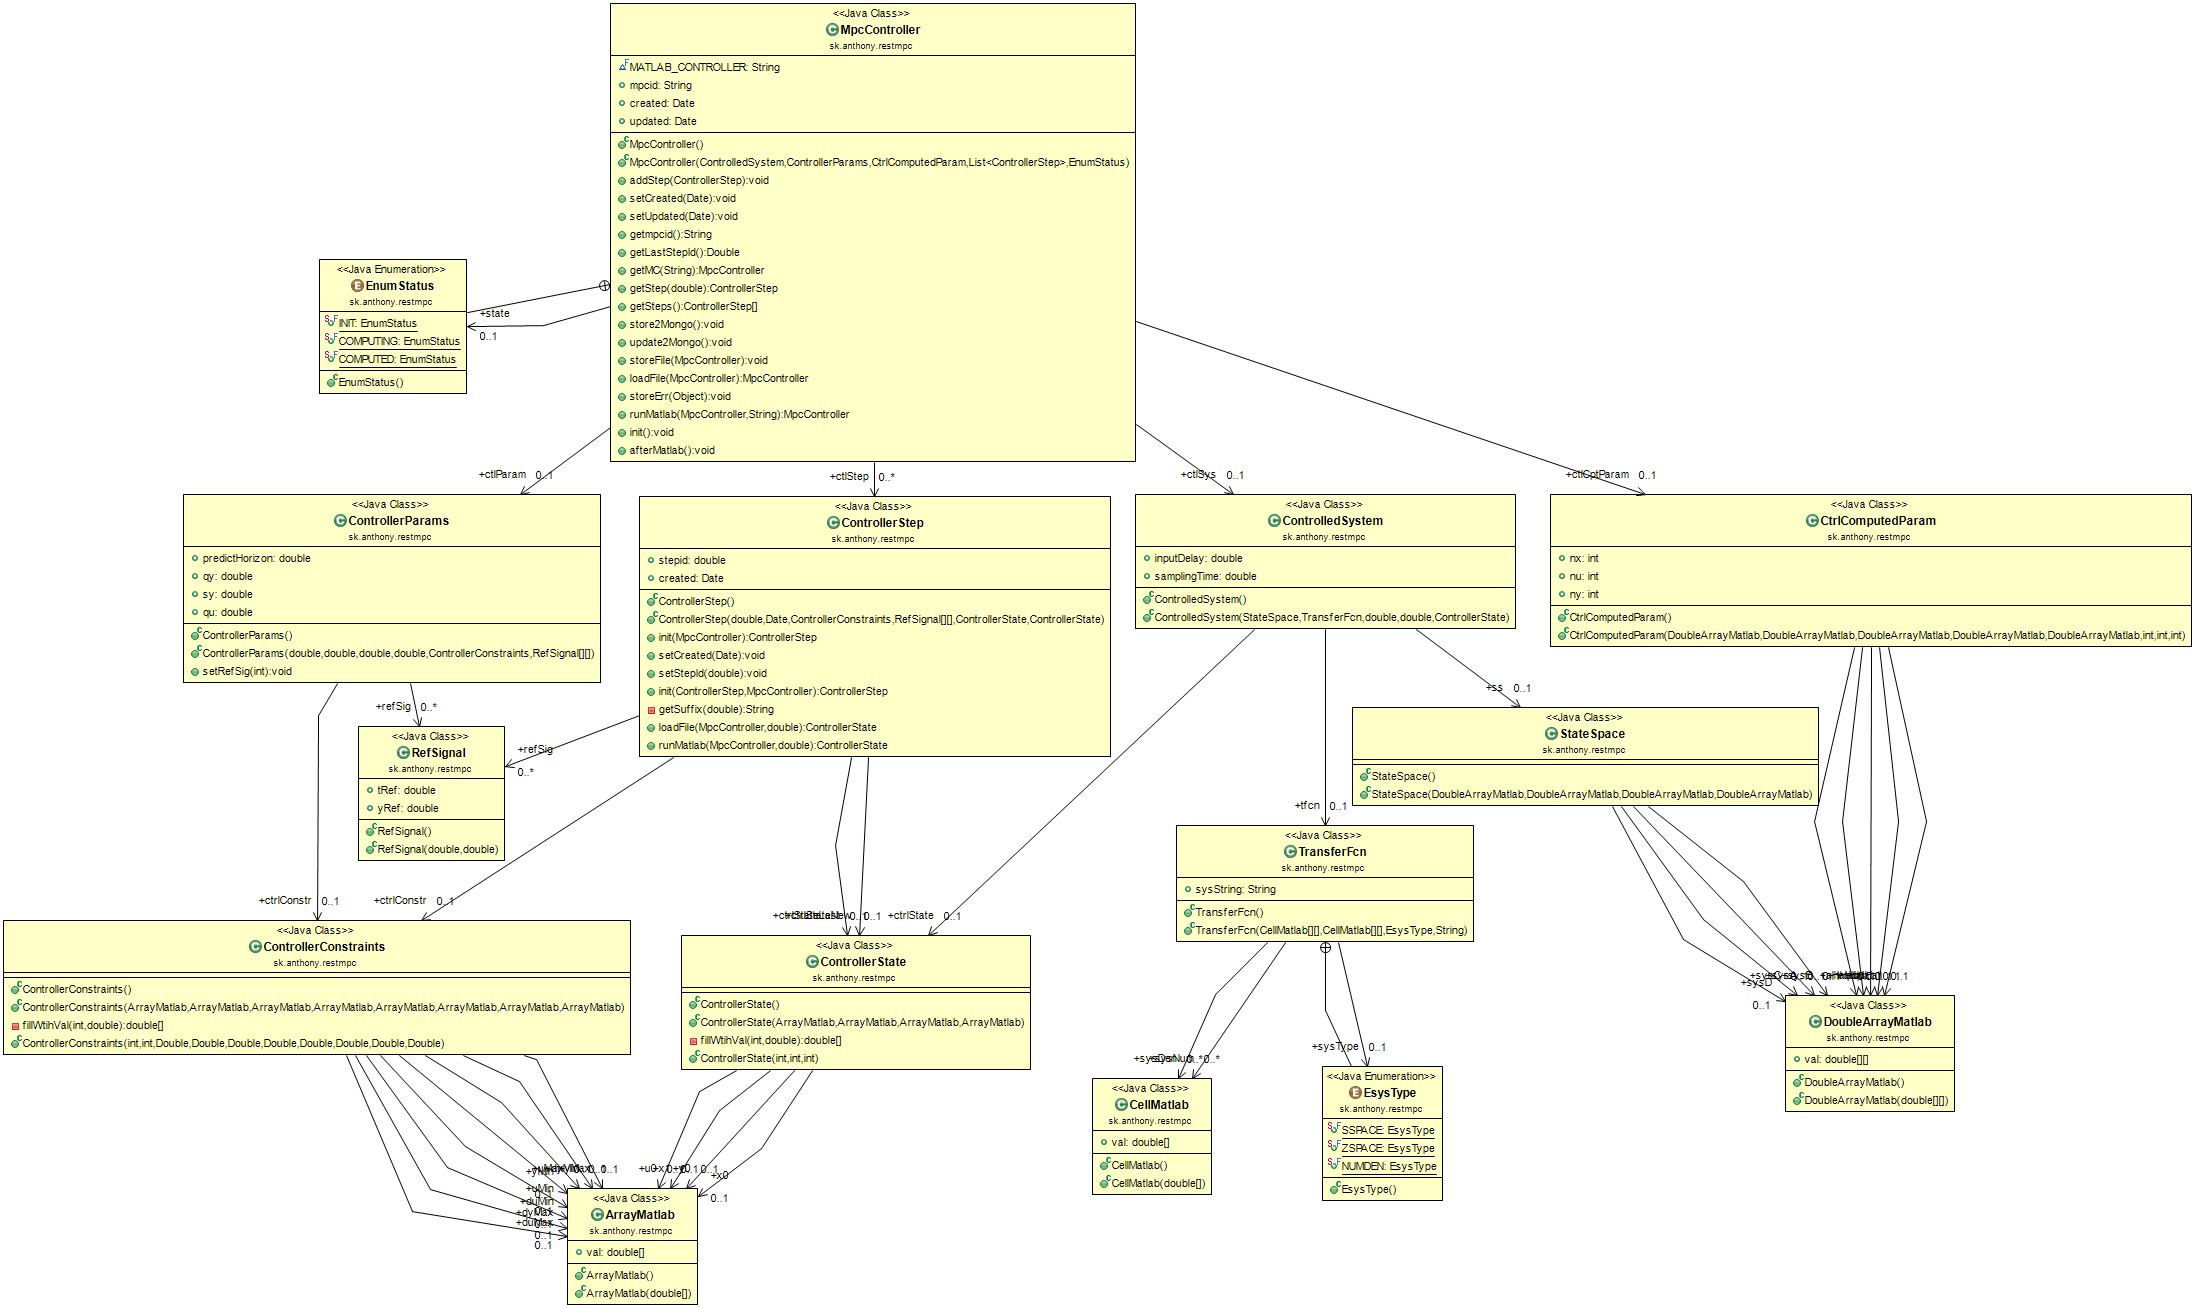
\includegraphics[width=1.5\textwidth]{39_class.png}
\caption{Diagram tried vstupného rozhrania.}
\label{39_class}
\end{figure} 
\end{landscape}

Funkcionalita, ktorú musí rozhranie na servery vykonať pri vytváraní inštancie regulátora a rovnako aj pri výpočte akčného zásahu pozostáva z týchto krokov:
\begin{enumerate}
  \item Inicializácia nenastavených default premenných.
  \item Uloženie do Mongo databázy, ktorá vygeneruje ID záznamu, ktoré figuruje ako ID regulátora.
  \item  Pred výpočtom sa uloží JSON do súboru.  
  \item Nasleduje volanie výpočtového systému Matlab alebo
   Octave, ktorý načíta uložený súbor, pomocou pluginu Jsonlab \cite{IOT29}, ktorý vie z JSON objektu spraviť Matlab/Octave dátové typy a naopak.
  \item Nasleduje krok v Matlab/Octave nástroji, kde prebehne výpočet podľa kapitoly \ref{mpcalg}, či už inicializácia systému alebo výpočet akčného zásahu. Na konci výpočtu sa dátové typy uložia do súboru pomocou Jsonlab vo forme JSON objektu.
  \item Späť v Java aplikácii sa súbor načíta a spraví z neho inštancia príslušnej triedy. 
  \item Upravený objekt sa uloží do databázy.
  \item Ten istý objekt sa pošle používateľovi na výstup.
\end{enumerate} 
Pri implementácii boli komplikácie s načítavaním objektu zo súboru, ktorý ukladal Jsonlab. Chýbala typová striktnosť, takže sa stalo, že z premennej typu vektor v Java aplikácii sa v Matlab/Octave stalo obyčajné číslo, ak vektor pozostával z jedného prvku. Následne pri ukladaní výsledkov výpočtov do súboru sa vynechala vektorová notácia a keď typovo striktný Java interface vytváral objekt, ktorý poskytne klientovi, tak vektorová notácia bola očakávaná. Na vyriešenie týchto komplikácii, boli potrebné úpravy do jadra Java objektov poskytujúcich transformáciu textu na JSON objekty. 

\indent Ďalší problém bol s volaním Matlab z inej aplikácie, kedy nebolo možné spustiť Matlab pod používateľom, ktorý je prihlásený ako vlastník procesu aplikačného serveru, pomocou ktorého je CaaS aplikácia spustená. Preto bol potrebný Python Interface, ktorým sa Matlab podarilo spustiť. Veľkú časť výpočtového času zaberá spustenie aplikácie Matlab. Preto bola vyskúšaná verzia spustenia Octave na Linux prostredí a čas výpočtu sa skrátil z v priemere 14 sekúnd na približne 4 sekundy. Pritom zariadenie s Linuxom bolo oveľa menej výkonné. Porovnanie parametrov v tabuľke  \ref{table:2}.
\begin{table}[h!]
\centering
 \caption{Porovnanie testovaných prostredí.}
 \begin{tabular}{ |p{4cm}|p{5.5cm}p{5.5cm}| } 
 \hline
 Procesor typ: & Intel Core i5-2520M & Intel Celeron M \\ 
  \hline
 Procesor frekvencia &  2.5GHz  & 1.46GHz   \\ 
 \hline
 Operačná pamäť: & 8GB & 2GB  \\ 
 \hline
 Disk & SSD & HDD \\
 \hline
 Operačný systém & Windows 8.1 & Debian 8 \\ 
 \hline
 Aplikácia & Matlab 2015 & Octave 3.6.2 \\  
 \hline
\end{tabular}
\label{table:2}
\end{table}
Tento fakt naznačuje preferenciu používania Octave verzie. 4 sekundy sa stále môžu zdať veľa, preto treba upozorniť, že ak by požiadavky na kvalitu regulácie boli striktnejšie je potrebné aplikáciu CaaS dať na výkonnejší stroj. Pri  načítaní regulátora z databázy je výsledok okolo 400 ms na slabšom zo spomínaných prostrediach. Preto pri riadení je možné očakávať podobné časy odpovede a teda na výkonných cloud zariadeniach je možné riadiť procesy s periódou vzorkovania rádovo desiatky milisekúnd. Spôsob garancie odpovede do určitého času a núdzový režim v prípade sieťového výpadku nie je v práci riešený. Dnes však poskytovatelia cloud služieb a poskytovatelia internetu vedia garantovať 24/7 dostupnosť a pripojenie.


\subsubsection{Integrácia MPC pomocou softvérového zariadenia} \label{integ}
Pre službu regulátora popísanú v predošlej časti a vystavenú v časti IoT Backend - obrázok \ref{35_schema} je potrebné vytvoriť klienta. V rámci práce je vytvorený klient v prostredí popísanom v kapitole \ref{iotenv}. Postup vytvorenia klienta aj súčasti potrebné na implementáciu sú podobné ako pri RSS Reader alebo REST Handler softvérových zariadení. Princíp ostáva rovnaký. Poskladať a zavolať HTTP požiadavku a spracovať odpoveď vo forme JSON správy, najskôr pre regulátor a potom cyklicky pre jednotlivé kroky, všetko v Lua jazyku vytvorené pre \textit{Luup} framework.\\
\indent Softvérové zariadenie vytvorené v práci je definované ako MpcClient s ID \textit{urn:demo-micasaverde-com:device:MpcClient:1} so službou, ktorá ma ID definované ako \textit{urn:demo-micasaverde-com:serviceId:MpcControl1}. Stavových premenných je tu viac ako v prípade RSS Reader zariadenia. Venovať sa budeme iba najdôležitejším. Spôsob vytvorenia inštancie zariadenia je rovnaký ako pre RSS Reader. Výhodou tohto prístupu je, že je možné vytvoriť viacero inštancií a riadiť nimi ľubovoľný počet akčných členov. Rozhranie na zadávanie parametrov a spustenie riadenia je na obrázku  \ref{40_mpccli}.
\begin{figure}[!htbp]
\centering
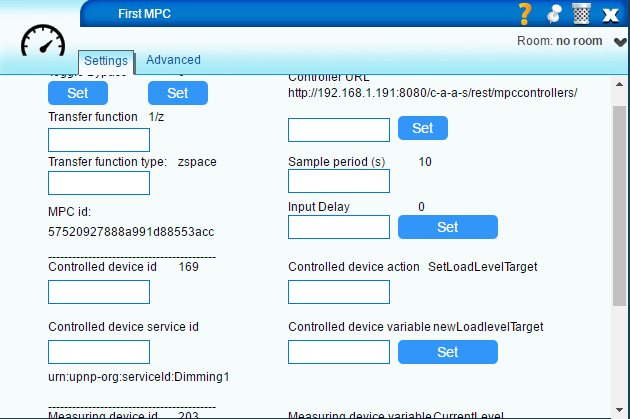
\includegraphics[width=0.85\textwidth]{40_mpccli.png}
\caption{Rozhranie na zadávanie parametrov MPC regulátora.}
\label{40_mpccli}
\end{figure} 
Nachádza sa tam
\begin{itemize}
  \item vstup pre prenosovú funkciu.
  \item Vstup pre zadanie URL služby, kde je aplikácia CaaS vystavená.
  \item Zobrazenie ID regulátora.
  \item Tlačítko na vypnutie/povolenie riadenia.
  \item Vstup pre zadanie periódy vzorkovania, ktorá zároveň identifikuje ako často sa bude volať služba na načítanie akčného zásahu.
  \item Vstupy na definovanie zariadenia, ktoré bude regulátorom ovládané.  
  \begin{itemize}
    \item ID inštancie zariadenia.
    \item ID služby.    
    \item ID operácie.    
    \item Meno vstupnej premennej do operácie.
  \end{itemize} 
  \item Vstupy na definovanie zariadenia, ktoré bude slúžiť na meranie výstupnej veličiny
  \begin{itemize}
    \item ID inštancie zariadenia.
    \item ID služby.    
    \item Meno meranej stavovej premennej.    
  \end{itemize}     
\end{itemize}
Princíp fungovania je taký, že na začiatku sa inicializuje regulátor zadaním prenosovej funkcie, snímacieho zariadenia, vykonávacieho zariadenia a periódy vzorkovania. Regulátor sa uloží do IoT Backend a na klientovi sa vždy na konci výpočtu načasuje spustenie nového výpočtu, ktorý sa spustí v čase periódy vzorkovania. Takto sa pravidelne zavolá IoT Backend, aby vrátil vypočítaný akčný zásah. Na vstupe je vždy nameraná hodnota zo snímacieho zariadenia, aby sa zabezpečila spätná väzba. Akčný zásah na výstupe je aplikovaný do akčného členu.

\indent Pri identifikácii systému, ktorá je popísaná neskôr, je identifikovaný nelineárny systém. Tento fakt spôsobuje, že na jeden proces sú potrebné viaceré regulátory pre každý pracovný bod lineárnej časti jeden. Na to aby bolo možné prepínať, ktorý regulátor ma riadiť danú časť priebehu je v práci vytvorené posledné šieste softvérové zariadenie s názvom MpcMaster. UPnP ID zariadenia je \textit{urn:demo-micasaverde-com:device:MpcMaster:1} a má jednu službu s UPnP ID \textit{urn:demo-micasaverde-com:serviceId:\textbf{MpcMultipleControl1}}. Operácie, definované v tejto službe sú:
\begin{itemize}
\item setSetpoint - slúži na stavenie žiadanej hodnoty
\item setMpcs - slúži na zadefinovanie ID softvérových zariadení MPC regulátorov (MpcClient), ktoré sú zodpovedné za riadenie jednotlivých priebehov, ďalej sa tu zadefinuje hranica, podľa ktorej sa rozhodne, ktorý regulátor bude vypočítavať akčný zásah a nakoniec slúži na samotné spustenie riadenia.
\item (un)setBypass - slúži na zastavenie riadenia.
\end{itemize}
Riadenie pozostáva z jednoduchých krokov.
\begin{enumerate}
\item Načítanie žiadanej hodnoty.
\item Rozhodnutie, ktorý MpcClient má byť spustený, 
\item Spustenie správneho MpcClienta, ktorý následne zavolá výpočet akčného zásahu a aj zabezpečí vykonanie akčného zásahu. 
\item Vypnutie MpcClienta, aby nezačal samostatne riadiť proces.
\item Nastavenie časovača, podľa periódy vzorkovania, kedy sa má  riadiaca slučka znovu spustiť.
\end{enumerate}
V prípade ak nad MpcClient zariadením preberá zodpovednosť MpcMaster, tak perióda vzorkovania, nastavená v zariadení MpcClient je ignorovaná, lebo zariadenie je plne pod správou MpcMaster. V tomto bode sú vytvorené všetky potrebné súčasti na riadenie pomocou prediktívneho regulátora v IoT prostredí.
\subsubsection{Experiment riadenia prostredníctvom MPC}
V tejto kapitole je vykonané overenie riadenia pomocou prediktívnej metódy v IoT prostredí. Samozrejme IoT prostredie je systém popísaný v kapitole \ref{iotenv}. Na experiment overenia riadenia sú využité tieto súčasti.
\begin{itemize}
\item Z fyzickej vrstvy sú využité zariadenia - stmievač FIBARO FGD 211 a fotorezistor pripojený na Raspberry Pi model B.
\item Na IoT bráne sú použité súčasti - softvérové zariadenia - 1x RestHandler na načítanie intenzity žiarenia, 2x MpcClient na získavanie hodnôt z IoT Backend časti, potrebných na riadenie a 1x MpcMaster na riadenie MpcClientov. 
\item Nakoniec je využitý IoT Backend popísaný v kapitole \ref{seccaas} na vykonávanie výpočtov prediktívneho regulátora.
\end{itemize}
Na overenie riadenia je zvolený proces udržiavania žiadanej intenzity svetla  pomocou svetelného zdroja, ktorý je ovplyvňovaný univerzálnym stmievačom FIBARO FGD 211 a pomocou fotorezistora, ktorý sníma intenzitu svetla.

\indent Ešte pred identifikáciou systému popíšeme spôsob prepočtu informácie z fotorezistora, ktorá je v jednotkách odporu (Ohm) na jednotku intenzity svetla (Lux). Na získanie referenčnej hodnoty intenzity svetla bol jednorázovo použitý lux meter typu PSH Ambient Light sensor od Intel inc., ktorý nie je pripojený do IoT systému. Údaje namerané v celom rozsahu stmievača v hodnotách po 10\% od 0\% po 100\% v testovacej miestnosti, sú zobrazene v grafe \ref{45_intrepolacia}, čiernými bodmi. Na osi x je hodnota rm - meraný odpor z fotorezistora a na osi y lm - meraná intenzita osvetlenia. Bodmi zobrazenými v grafe \ref{45_intrepolacia} je pomocou \textit{cftool} (Curve fitting tool) funkcionality nástroja Matlab preložená funkcia identifikujúca potrebný prepočet znázornená modrou farbou. Rozsah hodnôt fotorezistora je od 0 po 255, kde 0 je najsvetlejší a 255 najtmavší bod.
\begin{figure}[!htbp]
\centering
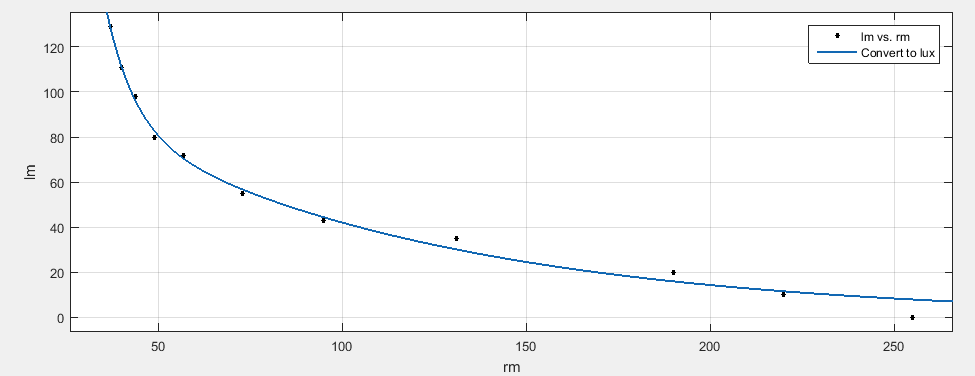
\includegraphics[width=0.85\textwidth]{45_intrepolacia.png}
\caption{Graf prepočtu odporu na intenzitu svetla.}
\label{45_intrepolacia}
\end{figure}

Matematický opis funkcie je:
\begin{equation} \label{eq42}
\begin{split}
f(x) = a*e^(b*x) + c*e^(d*x) \\
Koeficienty: \\
a =        5244 \\  
b =     -0.1279 \\ 
c =       123.2 \\ 
d =    -0.01074 
\end{split}
\end{equation}
Kde x je vstupný odpor a f(x) výstupná intenzita osvetlenia. Na základe toho, že fotorezistor, resp. AD prevodník dáva len hodnoty od 0 po 255 a že interpolačná funkcia je exponenciálna, treba zdôrazniť, že čím je intenzita osvetlenia väčšia tým je údaj nepresnejší a zároveň o to viac kolíše. V testovacej miestnosti sa intenzita pohybovala do 200 luxov (v závislosti od polohy merača), kde od hodnoty 140 luxov meranie začína kolísať v rozmedzí 40 luxov, čo uvidíme neskôr pri identifikácii. Tento fakt neskôr zohľadníme pri vyhodnocovaní kvality riadenia.

\indent Prejdeme k samotnej identifikácii systému. Na začiatku je vykonaná prevodová charakteristika zobrazená v grafe \ref{46_prevod_ch}. 
\begin{figure}[!htbp]
\centering
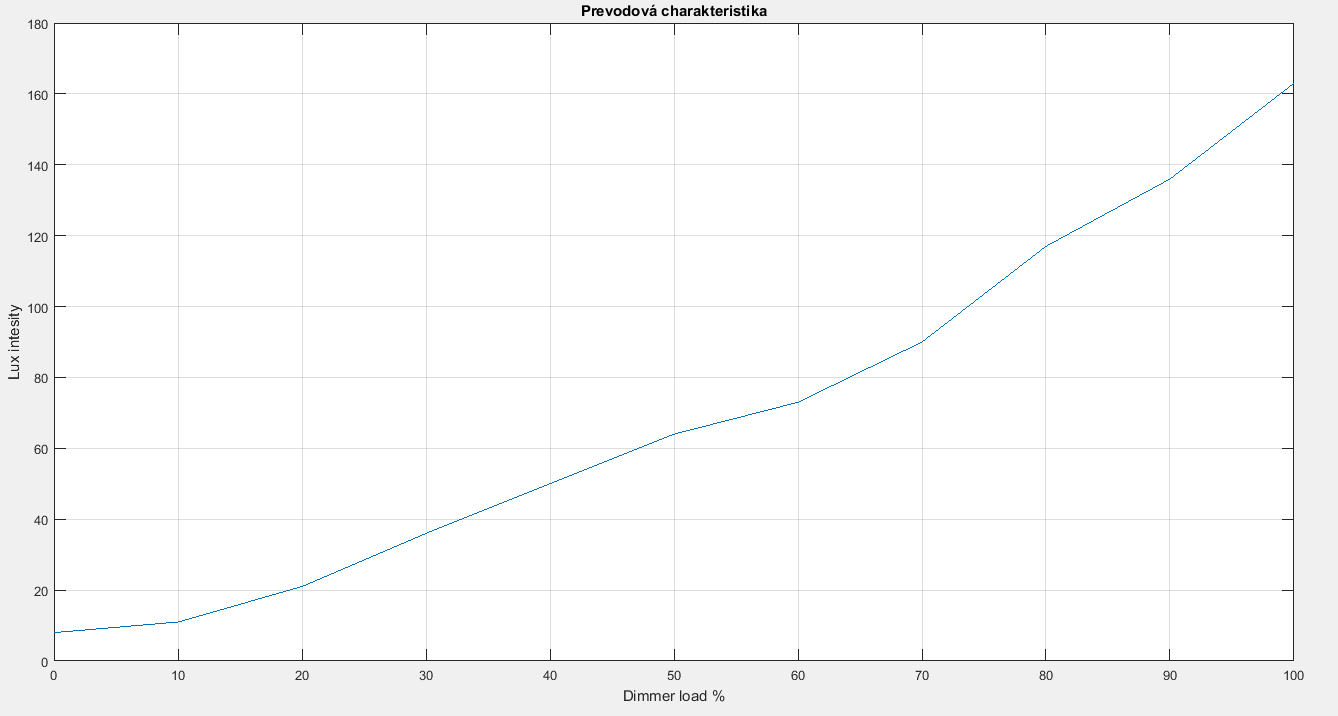
\includegraphics[width=0.85\textwidth]{46_prevod_ch.png}
\caption{Prevodová charakteristika závislosť intenzity osvetlenia od percenta zotmenia}
\label{46_prevod_ch}
\end{figure}
Na osi y je intenzita osvetlenia v luxoch a na osi x je miera zotmenia stmievača v \%. Z grafu je možné vidieť, že systém nie je lineárny. V prvej časti grafu od 20\% do 60\% na osi x je možné vidieť lineárnu oblasť, kde na zmenu o 40\% intenzita narástla o necelých 25 luxov na osi y. Potom  od 60\% do 100\% na osi x je druhá lineárna oblasť na zmneu 40\% intenzita narástla o viac ako 40 luxov na osi y. Na základe týchto dvoch oblastí sú zvolené dva pracovné body: miera zotmenia 30\% a 80\% na osi x. Hranica, ktorá tieto dve oblasti oddeľuje je približne 75 luxov na osi y. Po zvolení pracovných bodov je potrebné spraviť identifikáciu systému pre tieto dva body. Pri identifikácii bola perióda vzorkovania čítania hodnoty intenzity osvetlenia nastavená na 0.1 sekundy pri riadení je to nastavené už len na každých 5 sekúnd. Dáta namerané pre identifikáciu v pracovnom bode 30 sú zobrazené v grafe \ref{47_ident_input}. Dáta v tomto grafe sú už posunuté do bodu 0 vstup v percentách o 30\% a výstup systému o strednú hodnotu ustáleného skoku, čo je 48 luxov. 
\begin{figure}[!htbp]
\centering
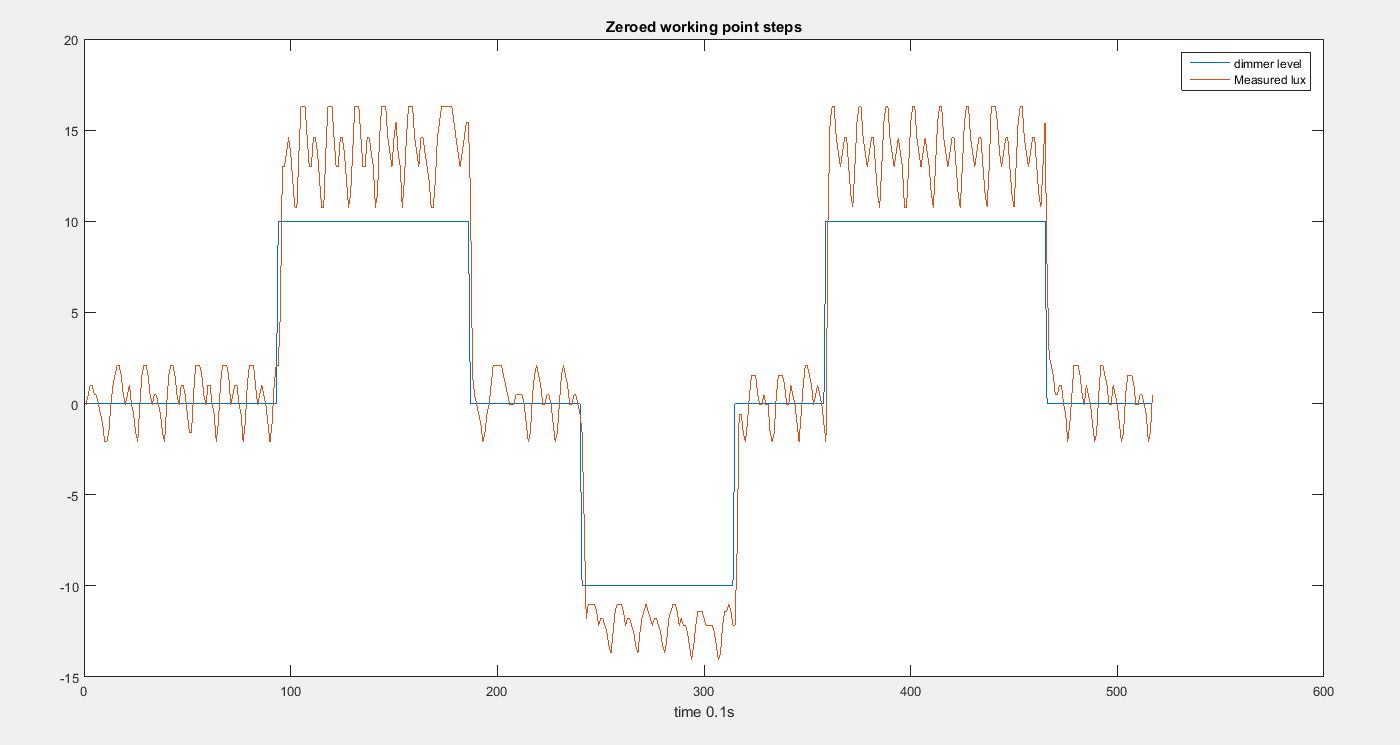
\includegraphics[width=0.85\textwidth]{47_ident_input.png}
\caption{Odozva systému v pracovnom bode 30, po posunutí hodnôt do bodu 0}
\label{47_ident_input}
\end{figure}
Následne namerané a posunuté dáta sa použijú na identifikáciu systému. Tá je vykonávaná prostredníctvom funkcionality \textit{ident} nástroja Matlab. Nástroj poskytuje viacero metód identifikácie, v experimente je použitá identifikácia prostredníctvom modelov prenosových funkcií, kde je zvolená identifikácia na systém 2. rádu. a pre porovnanie aj systém 3. rádu. Výstupné grafy identifikácie  sú znázornené na obrázku \ref{48_ident_out} a odozvy identifikovaných funkcií sú na obrázku \ref{49_ident_resp}.

\begin{figure}[!htbp]
\centering
\begin{subfigure}{0.5\linewidth}
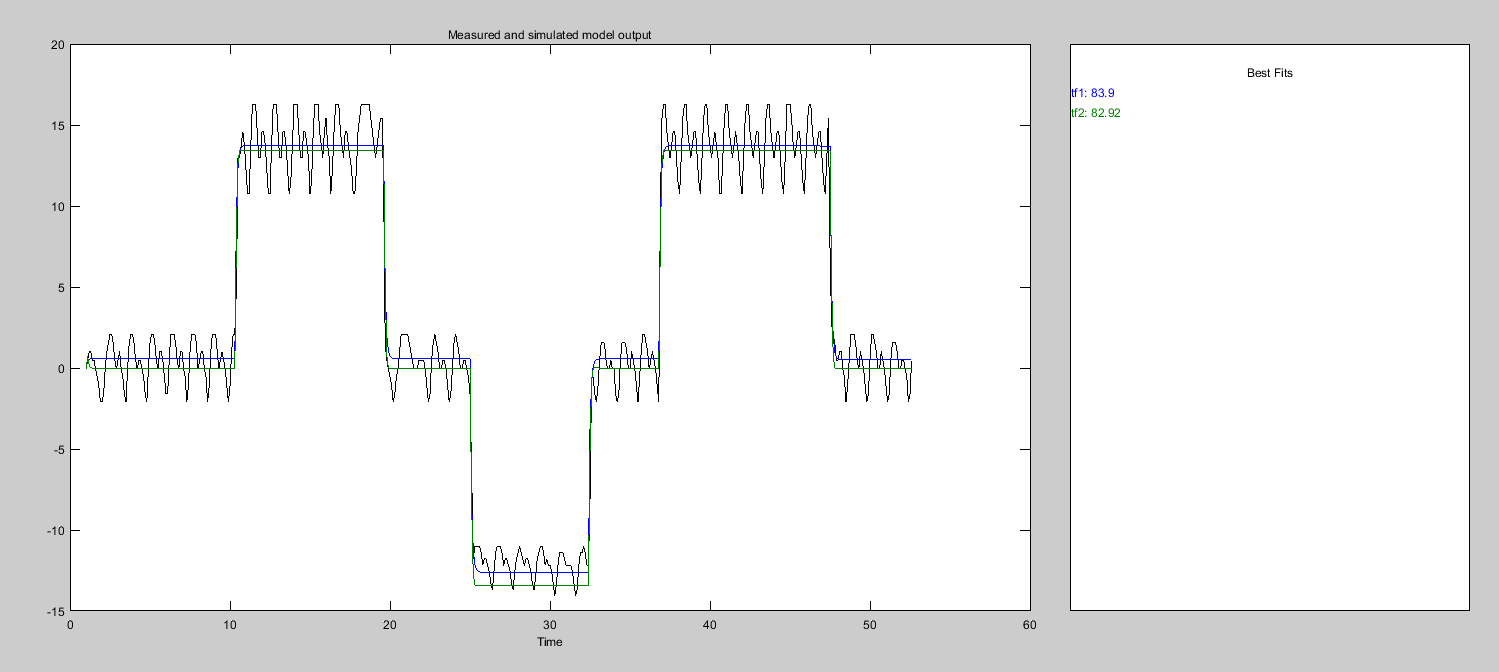
\includegraphics[width=0.9\textwidth]{48_ident_out.png}
\caption{Odozva na vstup pre bod 30.}
\label{48_ident_out}
\end{subfigure}%
\begin{subfigure}{0.5\linewidth}
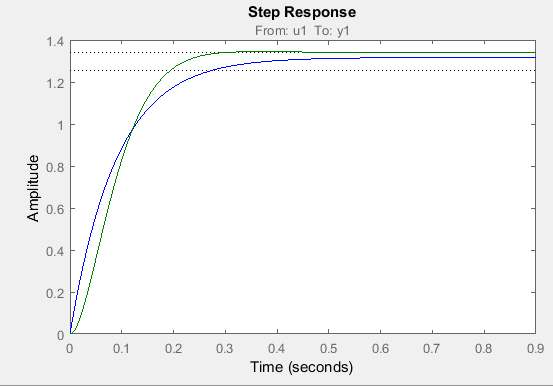
\includegraphics[width=0.9\textwidth]{49_ident_resp.png}
\caption{Prenosové funkcie pre bod 30.}
\label{49_ident_resp}
\end{subfigure}
\caption{Grafy identifikácie pre pracovný bod 30.}
\end{figure}

Na obrázkoch sú znázornené čiernou čiarou nameraný výstup, modrou farbou prechodová funkcia 2. rádu a zelenou farbou prechodová funkcia 3. rádu. Keďže funkcia 2. rádu presnejšie opisuje existujúci systém táto prechodová funkcia je vybratá na použitie do riadenia pomocou MPC, ktoré potrebuje matematický model. Táto prenosová funkcia má tvar:
\begin{equation} \label{eq40}
\begin{split}
 G_1 = \frac{14.71*s + 0.0291}{s^2 + 11.17*s + 0.0232}
\end{split}
\end{equation} 
Pred aplikovaním funkcie do procesu je  vyskúšaná v simulačnom nástroji opisovanom na konci prvej časti práce - kapitola \ref{mpcprogram}. Parametre a výstup simulácie sú na obrázkoch \ref{50_sim_param} a \ref{51_sim_out}.
\begin{figure}[!htbp]
\centering
\begin{subfigure}{0.5\linewidth}
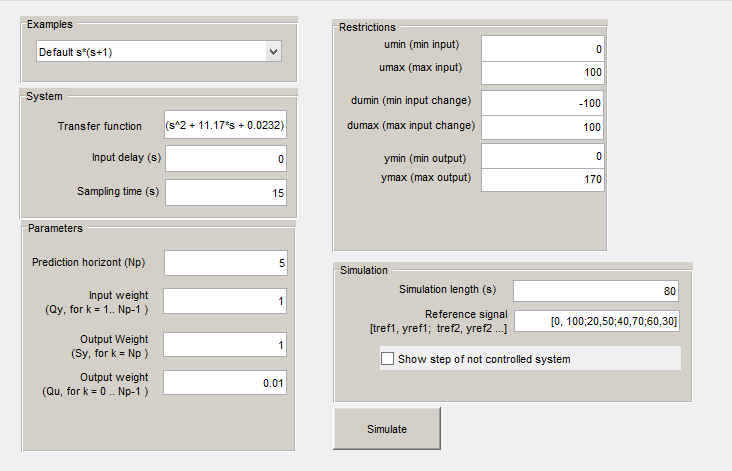
\includegraphics[width=0.9\textwidth]{50_sim_param.png}
\caption{Parametre simulácie pre prvú prenosovú funkciu}
\label{50_sim_param}
\end{subfigure}%
\begin{subfigure}{0.5\linewidth}
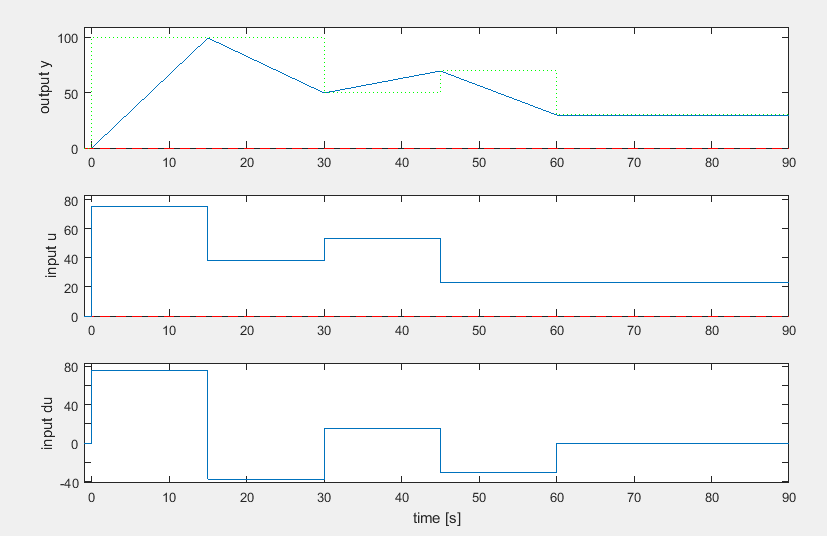
\includegraphics[width=0.9\textwidth]{51_sim_out.png}
\caption{Výstup simulácie pre prvú prenosovú funkciu}
\label{51_sim_out}
\end{subfigure}
\caption{Simulácia prenosovej funkcie.}
\end{figure}
Dôležité informácie na týchto obrázkoch sú voľba periódy vzorkovania až na 15 sekúnd. Táto hodnota je zvolená kvôli tomu, aby sme týmto jedným softvérovýhm zariadením a riadiacim procesom nevyťažili  zdroje VeraLite brány natoľko, že by ostatné funkcie fungovali bez oneskorenia.  Ďalej sú tu nastavené obmedzenia procesu tak, aby korešpondovali s reálnymi možnosťami zariadení. Obmedzenie na vstup je od 0 po 100 v našom prípade \% a zmena môže byť či už z 0 na 100 alebo zo 100 na 0, takže obmedzenia na zmenu vstupu sú na hodnotách -100 a 100. Nakoniec obmedzenia na výstup sú od 0 po 170 luxov. Váhy prediktívneho regulátora nie je potrebné meniť, pretože výstupná veličina sleduje žiadanú hodnotu s požadovanou kvalitou riadenia.
 
\indent Keď sme predchádzajúcou prenosovou funkciou dali riadiť systém v celom rozsahu, tak od hodnoty 100 luxov už dochádzalo k trvalým regulačným odchýlkam. Preto je nevyhnutné robiť identifikáciu pre druhý pracovný bod 80\%. Rovnaký postup ako pre bod 30 sa namerali údaje so skokmi okolo pracovného bodu. Namerané údaje je možné vidieť na obrázkoch \ref{52_schodynf80} a \ref{52_schody80}, opäť sú namerané dáta posunuté do bodu 0. V tomto prípade bol signál natoľko zašumený, že sme aplikovali filter pomocou pohyblivého priemeru (moving average) po 7 vzorkách takže za čas 0.7 sekundy. Na obrázkoch je vidieť rozdiel. Pre účely identifikácie bol zvolený odfiltrovaný signál, pretože identifikačný nástroj pre nefiltrovaný signál nedával vhodné modely. 

\begin{figure}[!htbp]
\centering
\begin{subfigure}{0.5\linewidth}
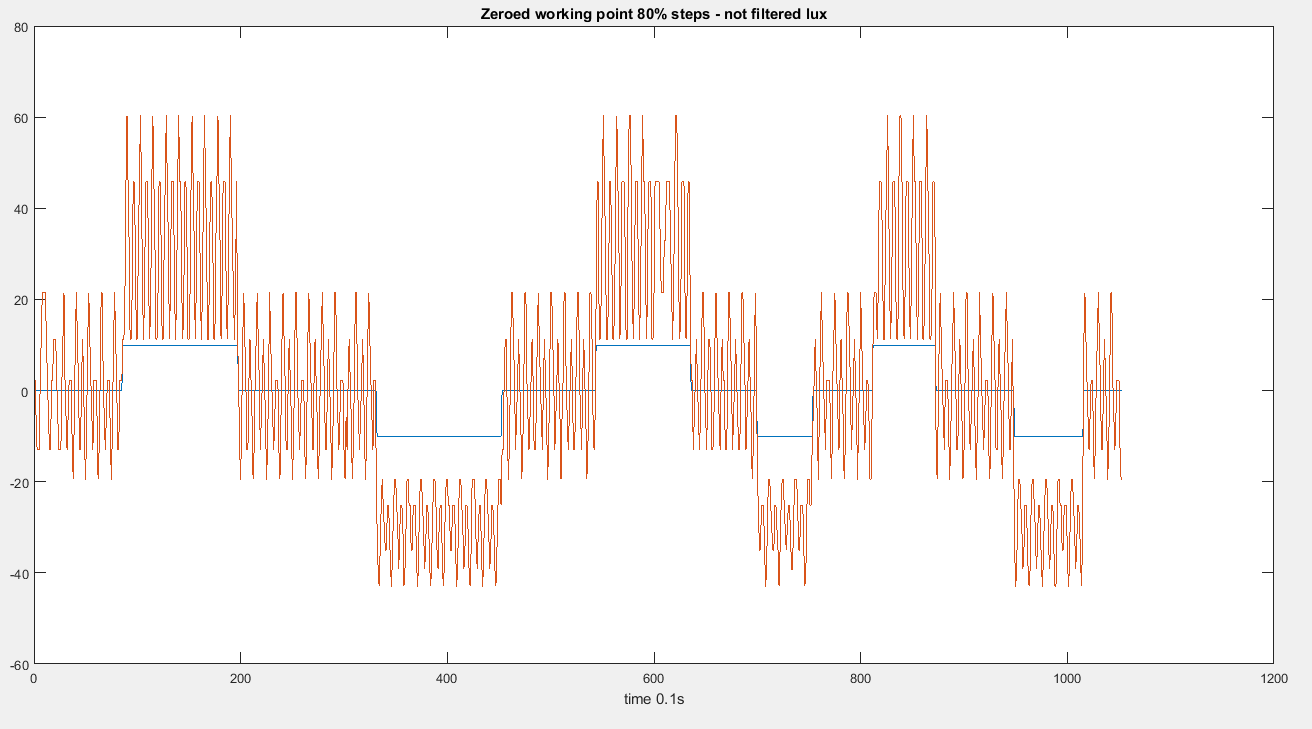
\includegraphics[width=0.9\textwidth]{52_schody80nf.png}
\caption{nefiltrovaná}
\label{52_schodynf80}
\end{subfigure}%
\begin{subfigure}{0.5\linewidth}
\includegraphics[width=0.9\textwidth]{52_schody80.png}
\caption{filtrovaná}
\label{52_schody80}
\end{subfigure}
\caption{Závislosť intenzity osvetlenia od percenta zotmenia v pracovnom bode 80\%. }
\end{figure} 
 
Po tom ako je signál odfiltrovaný ident funkcionalita vráti kvalitnejšie modely. Percento zhody je síce nižšie ako pri menej zašumenom signály v predchádzajúcom pracovnom bode, ale nemá to vplyv na kvalitu regulácie. Odozvy identifikovaného systému sú znázornené na obrázku \ref{53_ident80}, prechodová funkcia je na obrázku \ref{53_step80}.
\begin{figure}[!htbp]
\centering
\begin{subfigure}{0.5\linewidth}
\includegraphics[width=0.9\textwidth]{53_ident80.png}
\caption{Odozvy systému v pracovnom bode 80.}
\label{53_ident80}
\end{subfigure}%
\begin{subfigure}{0.5\linewidth}
\includegraphics[width=0.9\textwidth]{53_step80.png}
\caption{Prenosová funkcia systému v pracovnom bode 80.}
\label{53_step80}
\end{subfigure}
\caption{Grafy identifikácie v pracovnom bode 80.}
\end{figure}  
Matematický tvar prenosovej funkcie v pracovnom bode 80 je:
\begin{equation} \label{eq41}
\begin{split}
 G_2 = \frac{8.074*s + 57.6}{s^2 + 7.645*s + 18.4}
\end{split}
\end{equation}
Pre vypočítanú prenosovú funkciu sú vykonané simulácie, kde parametre a výstup sú znázornené na obrázkoch \ref{54_param80} a \ref{54_sim80}.
\begin{figure}[!htbp]
\centering
\begin{subfigure}{0.5\linewidth}
\includegraphics[width=0.9\textwidth]{54_param80.png}
\caption{Parametre simulácie pre druhú prenosovú funkciu}
\label{54_param80}
\end{subfigure}%
\begin{subfigure}{0.5\linewidth}
\includegraphics[width=0.9\textwidth]{54_sim80.png}
\caption{Výstup simulácie pre druhú prenosovú funkciu}
\label{54_sim80}
\end{subfigure}
\caption{Simulácie pre druhý pracovný bod.}
\end{figure}
V tomto prípade treba upozorniť na obmedzene na vstup, ktoré je nastavené od 0 po 65\%. Ako je možné vidieť v strednom grafe obrázku \ref{54_sim80} táto hodnota nie je dosiahnutá ani pri maximálnej intenzite osvetlenia, ktorá bola v miestnosti dosiahnutá - 200 luxov. V tejto simulácii je pracovný rozsah stmievača od 0 po 65\%. Tým, že merané hodnoty boli pri identifikácii posúvané k nule, ale hlavne tým, že systém nie je lineárny a dolnú časť má na starosti iný regulátor k akčnému zásahu regulátora pre hornú oblasť je potrebné vždy pridať 100-65 = 35\%.
Takto identifikované systémy a parametre sú aplikované do pripraveného IoT prostredia. 
\begin{enumerate}
\item Prenosová funkcia $G_1$ (\ref{eq40}) je aplikovaná do jednej inštancie MpcClient zariadenia. 
\item Prenosová funkcia $G_2$ (\ref{eq41}) je aplikovaná do druhej inštancie MpcClient zariadenia a offset akčného zásahu je nastavený na 35\%.
\item Na správu dvoch MpcClient zariadení je vytvorená jedna inštancia MpcMaster zariadenia, ktorá má na vstupe identifikované dve predošlé inštancie a hranicu 75 luxov žiadanej hodnoty ako rozhodujúcu. Ak je žiadaná hodnota pod touto hodnotou, tak MpcMaster volá prvú inštanciu regulátora, aby poskytla údaje o akčnom zásahu zo servera, ak je žiadaná hodnota vyššia, tak volá druhú inštanciu regulátora, ktorá je zodpovedná za získanie akčného zásahu zo servera a jeho uskutočnenie. 
\item Na zaznamenávanie údajov vo VeraLite zariadení je použité softvérove zariadenie dataMine \cite{IOT31} - plugin do VeraLite zariadenia, ktoré okrem ukladania umožňuje aj robiť grafy z nameraných údajov. Forma ukladania dát je v podobe časová značka, hodnota. Namerané dáta je potrebné ešte upraviť, pretože každé zariadenie má inú periódu vzorkovania, je potrebné ju zjednotiť. Na zjednotenie periódy vzorkovania je vytvorený jednoduchý skript v nástroji Matlab naznačený v algoritme  \ref{alg05}, ktorý prejde vektory vstupných časov a vstupných hodnôt a do každej ,,medzery`` medzi časmi vloží poslednú nameranú hodnotu. To isté sa spraví pre všetky veličiny, ktoré je potrebné zjednotiť, čím sa získajú dáta o perióde vzorkovania 1s pre všetky veličiny.
\end{enumerate}

\begin{algorithm}
\lstset{
    language=C,
    basicstyle=\small\sffamily,
    frame=none,
    numbers=left,
    xleftmargin=5.0ex,
    numberstyle=\tiny,
    stepnumber=1,
    showstringspaces=false,
    keywordstyle=\color{blue}\bfseries
    }
\lstset{emph={%  Adjust any special keywords
    printf%
    },emphstyle={\color[rgb]{1,0,0}\bfseries}%
}%
\begin{lstlisting}
function output=fillval(inputtime,inputvalue)
output = zeros(1,floor(inputtime(length(inputtime))));
for j=1:floor(inputtime(1))
    output(j)=inputvalue(1);
end

for i=2:length(inputtime)
    for j=floor(inputtime(i-1)):floor(inputtime(i))
        output(j)=inputvalue(i-1);
    end
end
\end{lstlisting}
 \caption{Príprava dát na identifikáciu}
 \label{alg05}
\end{algorithm} 
 
S takto pripravenými zariadeniami sa spúšťa proces riadenia pomocou tlačítka v MpcMaster zariadení, v ktorom sa rovnako postupne mení žiadaná hodnota. Zaznamenané zmeny nameranej veličiny a akčné zásahy sú v spomenutom DataMine zariadení. Ukážka grafov, ktoré pripravuje DataMine je na obrázku  \ref{41_vera_measurement}. Exportované a spracované dáta experimentu v Matlabe sú na obrázkoch \ref{42_set_lux} a \ref{43_mes_lux}.

\begin{figure}[!htbp]
\centering
\includegraphics[width=0.85\textwidth]{41_vera_measurement.png}
\caption{Namerané dáta pomocou DataMine.}
\label{41_vera_measurement}
\end{figure}

\begin{figure}[!htbp]
\centering
\includegraphics[width=0.85\textwidth]{42_set_lux.png}
\caption{Sledovanie žiadanej hodnoty výstupnou hodnotu intenzity osvetlenia.}
\label{42_set_lux}
\end{figure}


\begin{figure}[!htbp]
\centering
\includegraphics[width=0.85\textwidth]{43_mes_lux.png}
\caption{Závislosť meranej hodnoty od percenta zotmenia.}
\label{43_mes_lux}
\end{figure}

Na obrázku \ref{42_set_lux} vidieť modrou farbou žiadanú hodnotu a červenou farbou meranú výstupnú veličinu. Kroky žiadanej hodnoty sú na začiatku po 20 luxov až po 200. Následne je skok na 50 luxov, na 100 luxov a nakoniec na 20. Z tohto grafu nie je vidieť, v ktorom čase riadi akčný zásah iná inštancia MPC regulátor. Keďže pravidlo je pomerne jednoduché. prvé akčné zásahy vykonávala prvá inštancia, až kým žiadaná hodnota neprekročila úroveň 75 luxov. Potom až po 200 luxov vykonávala akčné zásahy druhá inštancia. Následne sa vystriedali a nakoniec posledné akčné zásahy vykonávala prvá inštancia. Ohľadne kvality regulácie môžeme vidieť, že po každej zmene žiadanej hodnoty je dopravné oneskorenie regulátora. To je spôsobene dvoma faktormi. Prvý je zvolená perióda vzorkovania 15s a druhý je čas výpočtu kroku, ktorý momentálne beží na zariadení, ktoré nemá požadovaný výkon. Keďže nejde o kritický proces naše požiadavky takéto dopravné oneskorenie akceptujú. Ďalej je možné pozorovať už spomenutý fakt nepresnosti a zašumenia merania intenzity osvetlenia pri vyššej intenzite. Do žiadanej hodnoty 100 luxov je stredná hodnota takmer zhodná so žiadanou. Následné hodnoty sú už viac zašumené, preto sa kvalita regulácie komplikovanejšie určuje. Avšak pri skokoch na 50 a 100 kedy sa testuje prepínanie regulátorov, je možné vidieť takmer nulovú regulačnú odchýlku. Pri žiadanej hodnote 20 luxov vidieť trvalá regulačnú odchýlku, ktorá je pravdepodobne spôsobená tým, že systém ma od 0 po 10 \% ďalšiu nelinearitu, ktorá nie je zohľadnená pri návrhu riadenia. Rovnakým princípom ako sú vyriešené 2 pracovné body, je možné vyriešiť N pracovných bodov. V rozsahu, kde sú stabilné merania, prediktívny regulátor riadi proces s výbornými ukazovateľmi kvality regulácie a princíp CaaS - vypočítania hodnôt akčných zásahov na servery je teda plne funkčný.

\indent Tento princíp je možné využiť napríklad na udržiavanie intenzity svetla so zapadajúcim slnkom. Ďalšie využitie výpočtového výkonu servera a neobmedzený počet regulátorov je na regulovanie teploty pomocou termostatu, ktorý v pripravenom IoT systéme je možné realizovať. Avšak experiment sa dial mimo vykurovaciu sezónu, preto nebolo možné uskutočnenie experimentu aj na tepelnom systéme. Možností využitia princípu CaaS sú týmto spôsobom neobmedzené, keďže pridanie ďalšieho regulátora je len vytvorenie novej inštancie. Stačí si zvoliť proces, ktorý treba riadiť, jeho akčný člen, senzor a identifikovať systém. Nakoniec spustiť riadiacu slučku. Pre lineárne procesy sa spúšťa na zariadení MpcClient pre nelineárne procesy pomocou viacerých MpcClientov a jedného MpcMaster zariadenia.

\subsection{Činnosti súvisiace s uvádzaním IoT systému do praxe}
Táto kapitola sumarizuje praktické skúsenosti z návrhu, realizácie a udržiavania IoT systému. Zdôrazňuje výhody, ale aj výzvy, ktoré  IoT a teda vytváranie užšej väzby medzi IT (informačnými technológiami) a OT (operačnými technológiami) prináša. Kapitola porovnáva činnosti potrebné pre čisto softvérové systémy a činnosti potrebné pre IoT systémy. 
\subsubsection{Návrh systému}
Základný nástroj pri návrhu softvérových systémov je modelovací nástroj s podporou napr. UML. V ňom sa modelujú základné prípady použitia systému, komponenty systému, sekvenčné diagramy a diagramy aktivít. Táto časť je spoločná pre oba typy systémov. Pre oba typy systémov sa volia programovacie jazyky pre jednotlivé komponenty a spôsob komunikácie medzi nimi. Pri IoT systémoch navyše zohráva veľkú úlohu výber hardvérových komponentov a protokolu, pomocou ktorého hardvérové komponenty budú podávať informácie. V prípade, že neexistuje zariadenie, ktoré by spĺňalo požiadavky finálneho systému je potrebné riešiť návrh samotných hardvérových komponentov, čo je ďalšia rozsiahla tematika. Rovnako výber vhodného protokolu je neľahká úloha. Ako možno vidieť na obrázku \ref{31_iot} v časti komunikačná úroveň, na ktorom zďaleka nie sú vymenované všetky existujúce protokoly, sú rôzne typy protokolov na rozličné spôsoby použitia. Ich využitie výhody a nevýhody sa líšia a všetky sa v čase vyvíjajú. To v praxi znamená, že pri návrhu je potrebné mať prehľad o protokoloch a zmenách v čase. Ďalšia oblasť pri návrhu systému je jeho bezpečnosť. V softvérových systémoch ide len o kybernetickú bezpečnosť, zatiaľ čo pri IoT systémoch treba dbať aj na fyzickú bezpečnosť. Ohľadne kybernetickej bezpečnosti v IoT systéme treba povedať, že IoT systém vystavuje viacero miest potenciálnych útokov a systém je tak bezpečný ako jeho najzraniteľnejšie miesto. Ak sa pozrieme na IoT systém popisovaný v kapitole \ref{iotenv}, tak ide o systém, ktorý je v rámci lokálnej domácej siete a preto zabezpečenie nie je na úrovni systému podnikovej siete a určite nie na úrovni siete internet.  O tomto systéme môžeme povedať, že je tak bezpečný ako je zabezpečený prístup do domácej siete, ale zároveň aj zabezpečenie siete Z-Wave, ktorá je bezdrôtová a teda je možné ju jednoducho odpočúvať. Nevyhnutnosť v obidvoch prípadoch, Z-Wave aj Wifi, je šifrovanie komunikácie. Ďalší bod zabezpečenia je prípojka do internetu vo väčšine domácich sieti zohráva túto úlohu router. Tu je nevyhnutné zamedziť nežiadúcim prístupom z internetu do lokálnej siete. Na druhej strane treba povoliť prístup žiadúcim prístupom napríklad pre prípad ovládania na diaľku. V popisovanom systéme je tento bod vyriešený VPN server aplikáciou bežiacou na routeri, ktorá umožňuje klientom, prostredníctvom vydaných certifikačných kľúčov, sa naň pripojiť a po pripojení ovládať zariadenia lokálnej siete. Ďalší aspekt týkajúci sa bezpečnosti domácej siete je úroveň oprávnenia na rôzne typy úkonov pri správe. Tento nedostatok sa dá vytknúť zvolenému zariadeniu VeraLite, ktoré má iba dve úrovne Admin a Guest, kde admin môže všetko ovládať aj konfigurovať a Guest môže všetko ovládať. Chýba obmedzenie na ovládanie len určitej množiny zariadení, ktoré môže hosť ovládať. Časť o kybernetickej bezpečnosti uzatvárame tým, že je nevyhnutné mať znalosti o spôsoboch zabezpečenia IT, ktoré podľa možnosti aplikovať na OT. Téma fyzickej bezpečnosti je na druhej strane viac rozpracovaná v OT pri návrhu výrobných liniek a podobne. V IoT systémoch sa kybernetická bezpečnosť spája s tou fyzickou, keď napríklad hovoríme o zásuvkách, dverách, chladničkách ovládaných na diaľku, ak sa pozeráme len v merítku oblasti inteligentných budov. O to viac prepojenie narastá v oblasti systémov pre spojené autá, inteligentnú mestskú infraštruktúru a podobne. V tomto bode IoT systémy otvárajú viaceré legislatívne otázky týkajúce sa zodpovednosti za spôsobené škody akýmkoľvek IoT systémom. Právna oblasť bude ešte ovplyvňovať smer a návrhy IoT systémov.   
Preto ak by sme definovali pozíciu architekta IoT systému, jeho znalosti a kompetencie sú v týchto doménach, či technológiách.
\begin{itemize}
\item UML a znalosť možností programovacích jazykov potrebných na vytvorenie IoT Backend častí
\item znalosť senzorov, akčných členov (pohonov, relé, ventilov, ...)
\item znalosť protokolov a možností prepojenia jednotlivých protokolov na vytvorenie vrstvy IoT zariadení a IoT brán
\item v určitých prípadoch znalosť návrhu plošných spojov
\item bezpečnosť informačných systémov - autentifikácia a autorizácie na základe rolí, ...
\item bezpečnosť informačný sietí - šifrovanie komunikácie, VPN, ...
\item bezpečnosť zariadení
\item právne aspekty domén nasadzovania IoT systémov
\end{itemize}
Tento zoznam nie je kompletný, ale snaží sa zaznamenať najdôležitejšie postrehy z praxe a poukázať na komplexitu, ktorú IoT systémy k pôvodnej softvérovej architektúre pridávajú.
\subsubsection{Vývoj systému}
Vývoj softvéru a ako už bolo spomenuté aj hardvéru nepochybne patrí do činnosti uvádzania IoT systémov do praxe. Kapitola sa viac zameriava na softvér, pretože vývoj hardvéru v našom prípade nebol potrebný. Aktuálne pri vývoji IoT systému len zriedka postačí jeden programovací jazyk. Je to z dôvodu rôznych typov zariadení v jednom ekosystéme, s rôznymi nárokmi na výkon a na správanie. Ak začneme od najjednoduchších zariadení, tak firmvér zvyčajne býva písaný v jazyku C, samozrejme sú aj ďalšie alternatívy. V našom systéme firmvér nebolo potrebné písať, pretože väčšina zariadení bola zaobstaraná, aby fungovala so Z-Wave protokolom. Najbližšie k hardvéru je v práci poskytovanie údajov z fotorezistora, cez PCF8591 AD prevodník. Framework Node.js zohráva svojimi nízkymi nárokmi dôležitú úlohu pri vývoji aplikácii na zariadení typu Raspberry Pi. Zariadenie Raspberry Pi a jeho konkurenti zohrávaju tiež dôležitú úlohu pri zavádzaní IoT systémov. Sú to ideálne zariadenia na vytváranie prepojenia s IoT backendom. V našom prípade je ako rozhranie zvolené VeraLite zariadenie, ktoré však svojím výkonom a parametrami je s nimi porovnateľné. Vývoj na úrovni brán je stále s jazykmi s nízkymi nárokmi na výpočtový výkon, ale stále poskytujúce rýchlu odozvu. Ako už bolo spomenuté, tak vo VeraLite je použitý interpretovaný jazyk Lua, ktorého interpreter vykonáva funkcie knižníc napísaných v jazyku C. V oblasti inteligentných domov je často v bráne (agregátore) vizualizácia pre koncového používateľa. Rozhranie prístupné na VeraLite zariadení je optimalizované pre Z-Wave zariadenia s možnosťou integrácie ďalších typov. Vo svete existujú aj projekty typu openHAB \cite{IOT32}, ktoré sa tvária nezávisle od protokolu, ktorým sú zariadenia pripojené. Tieto nástroje služia ako softvér na vytvorenie centrálnej brány v lokálnej sieti a zastávaju funkciu správy a vizualizácie zariadení. Základne prvky automatizačných funkcií sú tiež podporované na tejto úrovni zariadení. Čo sa týka nezávislosti na protokole v konečnom dôsledku je potrebný plugin, aby určitý typ zariadení podporovaný bol. Keď si zoberieme napríklad Z-Wave protokol, tak na to, aby boli vo vizualizácii Z-Wave zariadenia zobrazené, musí byť naprogramovaný plugin, ktorý to umožní. Takže veľmi podobný prípad, ako integrovanie iných zariadení do VeraLite brány. Zhrnúť to môžeme tak, že mať vizualizáciu ešte v lokálnej sieti je takmer nevyhnutné, aby bolo možné riadiť dom aj v prípade výpadku internetu, ktorá vizualizácia sa zvolí je takmer jedno, na jednej strane vždy treba niečo integrovať. Ďalšia súčasť IoT systémov je IoT backend, ktorého vývoj sa najviac podobá existujúcim čisto softvérovým systémom. Na tejto úrovni sú dátové body natoľko abstraktné, že IoT backend nemusí rozoznávať, akým spôsobom boli získané. Faktor, ktorý sem vstupuje je množstvo dát. Systém nemusí byť IoT, aby spracovával veľa údajov, avšak už bolo spomenuté, že s IoT sa často spája pojem Big data. Toto je práve oblasť, ktorú treba zvládnuť na IoT backende a ktorá dáva IoT systému ďalšiu pridanú hodnotu. Okrem štandardných jazykov, platforiem a databáz, ktorými sa aplikácie programujú, je potrebné sledovať vývoj nových jazykov, platforiem, databáz. V práci je použitý aj klasický prístup na aplikovanie moderných metód riadenia, kde je zvolený jazyk Java, ako jeden z najstabilnejších a najpoužívanejších. Ako úložisko je použitá MongoDB databáza, ktorá je menej konvenčná, ale trendy ukazujú, že čo chvíľa sa z nej stane konvenčná  databáza. Oproti tradičným relačným databázam typu MySQL sa líši tým, že nemá tabuľky, ale kolekcie dokumentov a nemá riadky a stĺpce, ale dokumenty a atribúty dokumentu a štruktúra atribútov nie je definovaná. Ďalej je v práci vyskúšaný jeden z moderných prístupov spracovania dát. Základné súčasti, ktorými sa Big Data zaoberá sú spracovanie, uloženie, vizualizovanie, analyzovanie a vyhodnocovanie veľkého objemu dát. Oproti v práci spomínaným komerčným platformám MS AZURE IOT HUB, AMAZON AWS IOT existujú aj open source platformy na prácu s dátami. V čase písania práce perspektívne vyzerajúce sú dve sady nástrojov. Jedna z nich je ELK \cite{IOT34} sada a druhá TICK \cite{IOT33} sada. Prvá je prezentovaná ako výborný nástroj na sledovanie logov, samozrejme využitie nie je limitované. Druhá je prezentovaná ako výborný nástroj na prácu s časovými radmi opäť využitie nie je limitované. Druhá menovaná je v práci vyskúšaná avšak len 3 nástroje zo štyroch a ich výstup je možné vidieť na obrázkoch \ref{55_chladnicka}, \ref{56_senzory}, \ref{57_svetla} a \ref{58_dvere} . Štvrtý nástroj slúžiaci na analýzu dát zasahuje do oblasti ,,data science``, ktorá sa zaoberá machine learning, deep learning a štatistickými modelmi, čo je ďalšia rozsiahla téma. Základné vyhodnotenia anomálnych, rizikových stavov v našom systéme bežia už vo VeraLite bráne, ktorá základnú logiku podporuje. Avšak logika vyplývajúca z dlhodobo nazbieraných dát v práci vyhodnocovaná nie je. Z vizualizácii je možné potvrdiť fakty, ktoré sa pomerne ľahko dajú predpokladať.

\begin{figure}[!htbp]
\centering
\includegraphics[width=0.85\textwidth]{55_chladnicka.png}
\caption{Spotreba chladničky po mesiacoch.}
\label{55_chladnicka}
\end{figure}

\begin{figure}[!htbp]
\centering
\includegraphics[width=0.85\textwidth]{56_senzory.png}
\caption{Grafy, vlhkosti vzduchu, intenzity osvetlenia a teploty.}
\label{56_senzory}
\end{figure}

\begin{figure}[!htbp]
\centering
\includegraphics[width=0.85\textwidth]{57_svetla.png}
\caption{Počty zapnutí svetiel.}
\label{57_svetla}
\end{figure}

\begin{figure}[!htbp]
\centering
\includegraphics[width=0.85\textwidth]{58_dvere.png}
\caption{Počty otvorenia vchodových dverí.}
\label{58_dvere}
\end{figure}
Na obrázku \ref{55_chladnicka} je možné pozorovať spotrebu chladničky po mesiacoch, kde je vidieť, že v letných mesiacoch jej spotreba stúpa. Grafy na obrázku \ref{56_senzory} ukazujú základné ukazovatele životného prostredia. Grafy na obrázku \ref{57_svetla} zobrazujú počty zapnutí jednotlivých svetiel za deň a po hodinách časy a frekventované miestnosti nie sú prekvapujúce. Z grafov \ref{58_dvere} je možné odčítať otvorenia vchodových dverí, z čoho by sa dal určiť čas zvyčajného príchodu a odchodu domov.

Pole pôsobenia vývojára IoT systému je tak ako v prípade architekta IoT systému rozšírené. Rozdeliť by sa znalosti dali na skupiny.
\begin{itemize}
\item Programovanie IoT zariadení - jazyky blízke hardvéru.
\item Programovanie IoT brán - jazyky s nízkymi nárokmi na výkon, ale vysokými na rýchlu odozvu.
\item Programovanie IoT backend - zahŕňajúce aktuálne konvenčné technológie.
\item Programovanie IoT backend - zahŕňajúce nové rýchlo rozvíjajúce sa technológie na spracovanie a analýzu dát veľkých objemov, rýchlosti a variability.
\end{itemize}

\subsubsection{Prevádzka systému}
Posledná oblasť činností je údržba IoT systému. Čisto softvérové systémy spravujú administrátori, pre ktorých existujú nástroje, ktoré sledujú stav serverov a služieb bežiacich na serveroch. Rovnaká požiadavka je potrebná aj pre IoT systém, ktorý ale má viacero úrovni a pod kontrolou je potrebné mať všetky úrovne. Starosť o IoT backend a o IoT bránu sa nelíšia. Pre účely monitorovania systému je v práci použitý nástroj Nagios \cite{IOT35}. Tento nástroj umožňuje čiastočne konfiguračne a čiastočne implementačne doplniť sledovanie stavu rôznych zariadení. Pre klasické služby má pripravenú sadu použiteľnej konfigurácie. Na obrázku \ref{59_nagios} je znázornené grafické rozhranie, ktoré ukazuje stav hlavných zariadení a služieb bežiacich na nich.
\begin{figure}[!htbp]
\centering
\includegraphics[width=0.85\textwidth]{59_nagios.png}
\caption{Rozhranie na sledovanie stavu spustených zariadení.}
\label{59_nagios}
\end{figure}
Doplňujúci prvok k tomuto nástroju je v práci nainštalovaný vlastný mail server, ktorý zabezpečí poslanie notifikácie okamžite pri detekcii nefunkčnosti zariadenia alebo služby. Pre promptnejšie notifikácie sa to často rieši SMS bránou, ktorá odošle SMS pri probléme, toto však v práci vyskúšané nie je. Rozmer, o ktorý je IoT systém v tomto smere rozšírený je starosť opravu zariadení. Veľká téma rozpracovaná v oblasti OT, na ktorú je potrebné upozorniť, keď sa hovorí o tom, čo IoT systém prináša. Nevyhnutná požiadavka pri výbere zariadenia je, aby vedelo informovať o stave bateriek, aby sa dala plánovať ich výmena. Počas prevádzky od apríla 2014 na opísaných zariadeniach došlo viac krát k výmene bateriek na niektorých snímačoch, čo navyše pri niektorých zariadeniach nebol jednoduchý proces. V tomto intervale došlo aj k znefunkčneniu dvoch spínačov, ktoré bolo potrebné vymeniť. Na základe týchto skúsenosti zdôrazňujeme, že pri odovzdávaní IoT systému je dôležite, aby bolo dohodnuté, kto systém spravuje a aký je reklamačný model resp. proces nastavenia správneho fungovania systému.
